\pagestyle{mat}
\chapter{Conjuntos Numéricos}
\markboth{Módulo 1}{}

\section{Habilidades do SAEB}

\begin{itemize}
  \item Escrever números racionais (representação fracionária ou decimal finita) em sua representação por algarismos ou em língua materna ou associar o registro numérico ao registro em língua materna.
  \item Compor ou decompor números racionais positivos (representação
decimal finita) na forma aditiva, ou em suas ordens, ou em adições e
multiplicações.
  \item Identificar números racionais ou irracionais.
  \item Comparar ou ordenar números reais, com ou sem suporte da reta
numérica, ou aproximar número reais para múltiplos de potência de 10
mais próxima.
  \item Converter uma representação de um número racional positivo para outra
representação.
  \item Identificar um número natural como primo, composto, ``múltiplo/fator
de'' ou ``divisor de'' ou identificar a decomposição de um número natural
em fatores primos ou relacionar as propriedades aritméticas (primo,
composto, “múltiplo/fator de” ou “divisor de”) de um número natural à
sua decomposição em fatores primos.
\end{itemize} 

\section{Habilidade da BNCC}

\begin{itemize}
  \item EF09MA02.
\end{itemize}

\conteudo{Os números racionais e irracionais são duas categorias de números
importantes na matemática.

Os números racionais são todos aqueles que podem ser escritos na forma
de fração, ou seja, como a razão entre dois números inteiros. Eles podem
ser representados no formato decimal finito ou infinito periódico, como
1/2, 0,75 e 0,333\ldots{} Os números racionais incluem também os números
inteiros e fracionários.

Por outro lado, os números irracionais são aqueles que não podem ser
expressos na forma de fração. Eles possuem infinitas casas decimais não
periódicas, como pi (\Pi), a raiz quadrada de 2 (\sqrt{2}) e a constante
de Euler (e). Os números irracionais não podem ser representados como
uma fração simples de dois números inteiros.

Uma característica importante dos números irracionais é que eles são
infinitos e não repetitivos, o que os torna fundamentais para a
geometria e para outras áreas da matemática.

Em resumo, os números racionais são aqueles que podem ser escritos na
forma de fração, enquanto os números irracionais são aqueles que não
podem. Ambos os tipos de números são importantes e estão presentes em
diversas áreas da matemática e da ciência.}

\section{Atividades}

\num{1} Escreva se os números abaixo são \textbf{Racionais(Q)} ou 
\textbf{Irracionais (I)}.

\begin{escolha}
  \item 0,25

  \reduline{Decimal exato é racional.\hfill}

  \item \Pi

  \reduline{O número pi é irracional.\hfill}
  
  \item \frac{2}{7}

  \reduline{Toda fração é racional.\hfill}
  
  \item \sqrt{7}

  \reduline{A raiz quadrada de 7 não é exata, está entre os números naturais 2 e
  3, pois 2\textsuperscript{2} = 4 e 3\textsuperscript{2} = 9. Toda raiz quadrada não exata é irracional.\hfill}
  
  \item 2,1230012579\ldots{}

  \reduline{Este número é uma dízima \textbf{não} periódica, ou seja, irracional.\hfill}
\end{escolha}

\num{2} Localize na reta aproximadamente os locais correspondentes aos
valores abaixo:

\begin{figure}
\centering
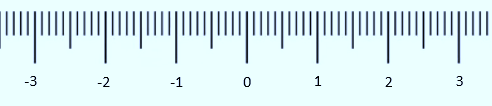
\includegraphics[width=4.10036in,height=0.88341in]{./_SAEB_9_MAT/media/image4.png}
\caption{Imagem em preto e branco Descrição gerada automaticamente com
confiança média}
\end{figure}

\begin{enumerate}
  \item \frac{2}{5}

  \item -- 1,8
  
  \item \sqrt{5}
\end{enumerate}

\num{3} Em um jogo realizado em sala de aula, o professor colocou
diversos números racionais e irracionais em uma urna. A primeira parte
do jogo consistia em cada grupo de alunos sortear 5 números sem reposição;
posteriormente, eles deveriam colocar os números sorteados em ordem
crescente. Os números sorteados por um destes grupos foram: 
7; \frac{9}{4} ; \sqrt{8} ; 0,75 e \frac{2}{3}. Escreva-os em ordem crescente.

\begin{boxmedio}
\coment{Considerando as aproximações \frac{9}{4} = 2,25; \sqrt{8} \approx 2,83;
0,75; e \frac{2}{3} = 0,66\ldots{} Temos: \frac{2}{3}; 0,75 ; \frac{9}{4} ; 
\sqrt{8} ; 7. 
\end{boxmedio}

\num{4} Complete a tabela.

\begin{center}
\begin{tabular}{|l|l|}
\hline
\textbf{Representação decimal ou fracionário} & \textbf{\begin{tabular}[c]{@{}l@{}}Descrição na língua materna\\ (escrito por extenso)\end{tabular}} \\ \hline
$\frac{2}{100}$ & \rosa{Dois centésimos} \\ \hline
$\rosa{\frac{3}{10}}$ & Três décimos \\ \hline
0,003 & \rosa{Três milésimos} \\ \hline
$\rosa{\frac{2}{1000}}$ & Dois milésimos \\ \hline
$\frac5{1}{100}$ & \rosa{Cinquenta e um décimos} \\ \hline
\end{tabular}
\end{center}

\num{5} Os números naturais podem ser primos ou compostos. Considerando
os números naturais 87 e 29, como podemos classificá-los? E quais os
critérios você utilizou para definir a classificação?

\begin{boxpeq}
\coment{O número 89 é composto, pois pode ser escrito como 3x29, 
e o número 29 é primo, pois não tem outro divisor primo.}
\end{boxpeq}

\num{6} Jorge adora propor desafios matemáticos para seus netos. No
último domingo disse para seu neto que em 2023 ele completou a idade
correspondente ao número de divisores positivos do número 5040. Quantos
aos completou Jorge no ano de 2023?

\begin{boxmedio}
\coment{Decompondo o número 5040 temos que: com isso o número de divisores
positivos são: (4+1)x(2+1)x(1+1)x(1+1) = 5x3x2x2=60. Desta
forma Jorge completou 60 anos em 2023.}
\end{boxmedio}

\num{7} Complete a tabela.

\begin{longtable}[]{@{}ll@{}}
\toprule
Representação decimal & Representação fracionária\tabularnewline
\midrule
\endhead
\rosa{2,4} & $\rosa\frac{24}{10}$\tabularnewline
2,712 & $\rosa{\frac{2712}{1000}}$\tabularnewline
0,0003 & $\rosa{\frac{3}{10000}}$\tabularnewline
0,25 & $\rosa{\frac{25}{100}}$\tabularnewline
\rosa{0,875} & $\frac{7}{8}$\tabularnewline
\bottomrule
\end{longtable}

\num{8} Decomponha os números abaixo em fatores primos.

\begin{escolha}
  \item 256

  \reduline{256 = 2\textsuperscript{8}\hfill}

  \item 1250

  \reduline{1250 = 2x5\textsuperscript{4}\hfill}

  \item 4800

  \reduline{4800 = 2\textsuperscript{6} x 3 x 5\textsuperscript{2}\hfill}

\end{escolha}

\num{9} Escreva o número que corresponde a cada fatoração em números primos.

\begin{escolha}
\item 2\textsuperscript{3} x 3\textsuperscript{2} x 5\textsuperscript{1}  

\reduline{360\hfill}

\item 3\textsuperscript{3} x 5\textsuperscript{2} x 7\textsuperscript{1}

\reduline{4725\hfill}
\end{escolha}

\num{10} Ao fazer a decomposição de 336 em fatores primos, Thiago chegou
à seguinte expressão 2\textsuperscript{x}x3x7. Qual valor Thiago deve 
colocar no lugar de x?

\begin{boxpeq}
\coment{Como o número 336 = 2\textsuperscript{4} x 3 x 7, temos que X 
é igual a 4.}
\end{boxpeq}

\section{Treino}

\num{1} Se o número 2\textsuperscript{3}\cdot3\textsuperscript{4}\cdot5\textsuperscript{X} tem exatamente 60 divisores positivos então o valor de X é:

\begin{escolha}
  \item 5
  \item 4
  \item 3
  \item 2
\end{escolha}

\num{2} Qual das 4 afirmações a seguir contém uma afirmação verdadeira? 

\begin{escolha}
\item
  Todo múltiplo de 5 é ímpar.
\item
  Todo número ímpar é múltiplo de 5.
\item
  Todo número par é múltiplo de 6.
\item
  Todo múltiplo de 12 é um número par. 
\end{escolha}

\num{3} Na reta numérica abaixo, há quatro valores indicados pelas
letras A, B, C e D. Qual destas letras indica a localização do número
1,6?

\begin{figure}
\centering
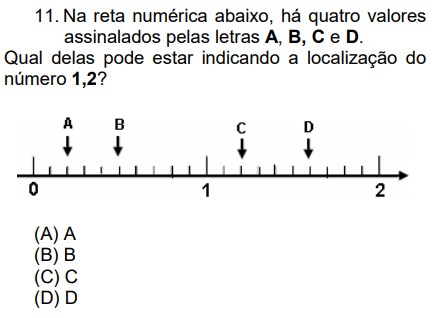
\includegraphics[width=3.66667in,height=0.85833in]{./_SAEB_9_MAT/media/image31.png}
\end{figure}

\begin{escolha}
  \item A
  \item B
  \item C
  \item D
\end{enumerate}

\chapter{Operações}
\markboth{Módulo 2}{}

\section{Habilidades do SAEB}

\begin{itemize}
  \item Calcular o resultado de adições, subtrações, multiplicações ou divisões
envolvendo número reais.
  \item Calcular o resultado de potenciação ou radiciação envolvendo números
reais.
  \item Resolver problemas de adição, subtração, multiplicação, divisão,
potenciação ou radiciação envolvendo número reais, inclusive notação
científica.
  \item Resolver problemas de contagem cuja resolução envolva a aplicação do
princípio multiplicativo.
  \item Resolver problemas que envolvam as ideias de múltiplo, divisor, máximo
divisor comum ou mínimo múltiplo comum.  
\end{itemize} 

\section{Habilidades da BNCC} 

\begin{itemize}
  \item EF09MA03, EF09MA04.
\end{itemize}

\conteudo{O conjunto dos números reais é a união entre o conjunto dos números
racionais e o conjunto dos números irracionais; dessa forma, o número
real pode ser um número racional ou um número irracional. Por isso, esse
conjunto também contempla o dos números naturais e o dos números
inteiros.

O conjunto dos números reais é o mais utilizado no cotidiano, como na
realização de medições, no cálculo de funções matemáticas, no estudo de
grandezas da física e da química, entre outras situações.

As operações envolvendo os números reais são:

\begin{itemize}
  \item Adição

  \item Subtração

  \item Multiplicação

  \item Divisão

  \item Potenciação

  \item Radiciação
\end{itemize}

A \textbf{potenciação} é a operação matemática que representa a
multiplicação de fatores iguais. Ou seja, usamos a potenciação quando um
número é multiplicado por ele mesmo várias vezes.

Notação:

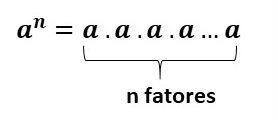
\includegraphics[width=1.46875in,height=0.63399in]{./_SAEB_9_MAT/media/image32.jpeg}

Sendo a \neq 0, temos:

\begin{myquote}
a: Base (número que está sendo multiplicado por ele mesmo).

n: Expoente (número de vezes que o número é multiplicado)
\end{myquote}

Para melhor entender a potenciação, no caso do número
4\textsuperscript{3} (quatro elevado à terceira potência ou quatro
elevado ao cubo), tem-se:

\begin{myquote}
4\textsuperscript{3} = 4 x 4 x 4 = 16 x 4 = 64
\end{myquote}

A \textbf{Radiciação} é o método matemático inverso à potenciação. Enquanto os
cálculos com potências são determinados pela multiplicação de elementos
iguais sucessivas vezes, a radiciação procura quais são esses elementos.

Por exemplo: se 8\textsuperscript{2} = 64, podemos dizer que a raiz quadrada de
64 é 8.
}

\section{Atividades}

\num{1} Urano é o sétimo planeta do Sol e é o terceiro maior no sistema
solar. Foi descoberto por William Herschel em 1781. Tem um diâmetro
equatorial de 51.800 quilômetros (32.190 milhas) e orbita o Sol uma vez
a cada 84,01 anos da Terra. Tem uma distância média do Sol de
2.870.990.000 quilômetros.

Escreva a distância média de Urano ao Sol em notação Científica.

\begin{boxpeq}
\coment{2,87 x 10\textsuperscript{9}km.}
\end{boxpeq}

\num{2} Jorge foi fazer uma entrega, em um condomínio, de 50 caixas
pesando 60kg cada caixa. Para cumprir essa tarefa, utilizou o elevador,
que tinha a capacidade máxima de 800kg. Jorge pesa 100kg. Por segurança,
o zelador não deixa que o limite de capacidade do elevador seja ultrapassado.

Quantas vezes será necessário usar o elevador para levar todas as
caixas?

\begin{boxmedio}
\coment{50 x 60 = 3000 kg de carga. Como Jorge tem 100 kg, é preciso considerar
que o limite de peso que pode ser colocado no elevador será de, no máximo, 700
kg. Para carregar 700 kg, Jorge deverá levar no máximo 11 caixas por vez.
50 : 11 = 4,54 aproximadamente, ou seja, 5 viagens.}
\end{boxmedio}

\num{3} Para fazer a publicação e um determinado livro, estimou-se um
custo inicial de R\$ 250.000,00 e ainda um custo de R\$ 10,00 por
unidade. Elisa quer publicar um livro com uma tiragem de 5.000
exemplares. Qual será o custo de cada exemplar?

\begin{boxmedio}
\coment{R\$ 250.000,00 + (5.000,00 x R\$ 10) = R\$ 300.000,00. 
Como serão publicados, 5.000 exemplares, é preciso
dividir o valor ou seja:  R\$ 300.000,00/5.000 = R\$ 60. 
Portanto, o custo por unidade é de R\$ 60,00.}
\end{boxmedio}

\num{4} A cantina da escola optou por vender lanches saudáveis e fez uma
negociação com o distribuidor de maçãs da região. A negociação fez com
que a cada duas maçãs fosse pago o valor de R\$ 0,80. O preço
de venda será de R\$ 1,00 por unidade.

Pretende-se um lucro mínimo semanal de R\$ 90,00 com as maçãs, dados os
custos operacionais internos.

Quantas maçãs precisam ser vendidas?

\begin{boxmedio}
\coment{Como o custo por unidade é de R\$ 0,40 e o valor de venda é R\$ 1,00,
o lucro por unidade é de R\$ 0,60. Dessa forma, para obter lucro mínimo 
semanal de R\$ 90,00, divide-se o valor pretendido (R\$ 90) pelo lucro 
por unidade (R\$ 0,60): 90/0,60 = 150 maçãs.}
\end{boxmedio}

\num{5} Uma xícara com leite pesa 420 g, porém se bebermos metade do
leite ele passa a pesar 230 g.

Qual o peso da xícara vazia?

\begin{boxpeq}
\coment{Ao analisar a diferença do peso da xícara cheia e com metade do leite,
percebe-se que houve redução de 190 g, ou seja, esta é massa ocupada
por metade do leite. Conclui-se, dessa forma, que o leite tem a massa de
190 x 2 = 380g e a xícara 420 -- 380 = 40g.}
\end{boxpeq}

\num{6} Leia o texto abaixo.

\begin{quote}
A NGC 4151 está localizada a cerca de 43 milhões de anos-luz
da Terra e se enquadra entre as galáxias jovens que possuem um buraco
negro em intensa atividade. Mas ela não é só lembrada por esses
quesitos. A NGC 4151 é conhecida por astrônomos como o `olho de Sauron',
uma referência ao vilão do filme \textit{O Senhor dos Anéis}.

\fonte{Folha de São Paulo. Galáxia herda nome de vilão do filme \textit{O Senhor dos Anéis}. Disponível em: http://www1.folha.uol.com.br/ciencia/887260-galaxia-herda-nome-de-vilao-do-filme-o-senhor-dos-aneis.shtml}
Acesso em: 8 mai.2023.}
\end{quote}

Para facilitar cálculos, números são utilizados em notação científica.
A notação científica do número \textbf{43 milhões de anos-luz}, do texto 
acima, está corretamente representada na alternativa:

\begin{minipage}{.5\textwidth}
\begin{escolha}
  \item 4,3 x 10\textsuperscript{7}

  \item 43 x 10\textsuperscript{7}

  \item 4,3 x 10\textsuperscript{--7}

  \item 43 x 10\textsuperscript{--7} 
\end{escolha}
\end{minipage}
\sidetext{43 milhões representam 43.000.000, ou seja, 43 X 10\textsuperscript{6}
ou 4,3 x 10\textsuperscript{7}.}

\num{7} Um professor de Educação Física quer mesclar os jogos que são
oferecidos para suas turmas e com isso estabeleceu uma regularidade de
repetição dos esportes das turmas. As partidas de futebol acontecem a 
cada 30 dias, as de basquete a cada 45 dias e as de handebol, a cada 60 dias.

Todas as modalidades foram oferecidas no dia de hoje. Quando essa
situação ocorrerá novamente?

\begin{boxpeq}
\coment{Determinando o MMC (30, 45, 60) = 180
A situação ocorrerá novamente após 180 dias.}
\end{boxpeq}

\num{8} Durante uma campanha de arrecadação de alimentos na escola,
a turma da Larissa arrecadou: 288 pacotes de feijão, 96 pacotes de açúcar,
360 pacotes de arroz e 240 pacotes de fubá. Larissa recorreu a seus
conhecimentos matemáticos para organizar pacotes que cada família
beneficiária receberia.

Quantos pacotes de feijão foram colocados em cada pacote para entregar,
considerando que o objetivo era atender a maior quantidade possível de
famílias?

\begin{boxmedio}
\coment{MDC (96, 240, 288, 360) = 24. Dessa forma, podemos determinar que, em
cada pacote, foram colocados 288/24 = 12 pacotes de feijão.}
\end{boxmedio}

\num{9} Uma costureira dispõe de dois pedaços de fita de comprimentos
1,20m e 1,80m. Ela pretende cortar essas fitas em pedaços menores e 
iguais, com o maior tamanho possível. Quantos pedaços menores de fita 
e de máximo tamanho possível ela conseguirá?

\begin{boxpeq}
\coment{MDC (1,20 e 1,80) = 0,60. Ela conseguirá cortar 2 pedaços da 
fita de 1,20 e 3 pedaços da fita de 1,80. Os pedaços serão de 60 cm.}
\end{boxpeq}

\num{10} Simplificando a expressão \sqrt[5]{\frac{2\textsuperscript{16}+2\textsuperscript{18}}{10}} encontramos

\begin{minipage}{.5\textwidth}
\begin{escolha}
\item 2
\item 4
\item 6
\item 8
\end{escolha}
\end{minipage}
\sidetext{
A alternativa correta é a D:
\sqrt[5]{\frac{2\textsuperscript{16}+2\textsuperscript{18}}{10}} = \sqrt[5]{\frac{2\textsuperscript{15} x (2\textsuperscript{1} + 2\textsuperscript{3})}{10}} = \sqrt[5]{\frac{2\textsuperscript{15} x 10}{10}} = 2\textsuperscript{3}
}

\section{Treino}

\num{1} Fernando faz caminhada a cada 4 dias. Thiago, vizinho de
Fernando, faz caminhada no mesmo parque, a cada 6 dias. Considerando que
Fernando e Thiago se encontraram sexta fazendo caminhada, em qual dia da
semana ocorrerá o próximo encontro entre eles?

\begin{escolha}
\item Segunda
\item Terça
\item Quarta
\item Sexta
\end{escolha}

\num{2} Para arrecadar dinheiro para a festa de formatura do 9º ano,
Julinha quer vender doces. Ela preparou 150 brigadeiros e 120 beijinhos,
e quer vender pacotes separados desses doces. Para facilitar as contas,
ela quer ter o mesmo número de pacotes de brigadeiros e de beijinhos, e
cada um desses pacotes deve conter o maior número possível de guloseimas. 
Quantos pacotes ela deve preparar? E quantos doces deve conter cada 
pacote?   

\begin{escolha}
\item
  30 pacotes de cada doce, 5 brigadeiros e 4 beijinhos.
\item
  10 pacotes de cada doce, 15 brigadeiros, 12 beijinhos.
\item
  15 pacotes de cada doce, 10 brigadeiros, 12 beijinhos.
\item
  90 pacotes de cada doce, 3 brigadeiros, 3 beijinhos.
\end{escolha}

\num{3} Leia o texto a seguir para responder à pergunta.

\begin{quote}
Cientistas australianos podem ter descoberto algo surpreendente nas
profundezas do mar: criaturas misteriosas, aparentemente vivas e tão
pequenas que chegam ao limite do que é necessário para que exista vida
independente.

Seus descobridores, da Universidade de Queensland, afirmam que esses
seres são novas formas de micróbios. Céticos, no entanto, veem a
descoberta como uma provável nova desilusão na caçada às menores formas
de vida.

Os pesquisadores as chamam de \textit{nanobes}. O ``nano'' vem de seu 
comprimento, de 20 a 150 nanômetros (bilionésimos de metro).

\fonte{William J. Broad. Equipe diz ter descoberto menor forma de vida.
Disponível em: https://www1.folha.uol.com.br/fsp/ciencia/fe1901200001.htm.
Acesso em: 9 mai. 2023.}
\end{quote}

O maior tamanho do nanobe em notação científica está corretamente
representado na alternativa:

\begin{escolha}
\item 15 x 10\textsuperscript{--7} m.
\item 1,5 x 10\textsuperscript{--7} m.
\item 150 x 10\textsuperscript{--9} m.
\item 1,5 x 10\textsuperscript{--9} m.
\end{escolha}

\chapter{Frações (associadas a imagens e fração geratriz)}
\markboth{Módulo 3}{}

\section{Habilidades do SAEB}

\begin{itemize}
  \item Representar frações menores ou maiores que a unidade por meio de
representações pictóricas ou associar frações a representações pictóricas.
  \item Identificar frações equivalentes.
  \item Determinar uma fração geratriz para uma dízima periódica.   
\end{itemize} 

\conteudo{
A fração geratriz é aquela cujo resultado será uma dízima periódica 
(número decimal periódico) quando calculamos seu valor decimal.

Os números decimais periódicos apresentam um ou mais algarismos que se
repetem infinitamente. Esse algarismo ou algarismos que se repetem
representam o período do número.

A fração geratriz pode ser determinada por meio de operações com equações
ou de algumas regras práticas que podem facilitar seu processo de
identificação.

O processo por equação pode ser realizado da seguinte forma:

\begin{itemize}
  \item Igualar a dízima periódica a uma incógnita, por exemplo x, de
forma a escrever uma equação do 1º grau;

  \item Multiplicar ambos os lados da equação por um múltiplo de 10
(a depender do número de casas em que ocorre a repetição dos termos);

  \item Subtrair a equação encontrada da equação inicial;

  \item Isolar a incógnita.
\end{itemize}

\textbf{Exemplo 1}

0,232323...

x = 0,232323...

100x = 23,232323...

100x -- x = 23,23232323... -- 0,232323...

99x = 23

x = \frac{23}{99}\

\textbf{Exemplo 2} 

0,5123123123...
Neste exemplo, temos um dígito após a vírgula que não se repete (5). 
É necessário, assim, fazer dois passos, para que apenas os
dígitos que se repetem fiquem após a vírgula.

x = 0,5123123123...

10x = 5,123123123...

10000x = 5123,123123...

10000x -- 10x = 5123,123123... -- 5,123123123...

9990x = 5118

x = \frac{5118}{9990}
}


\section{Atividades}

\num{1} Dados dois números reais x e y, tais que x = 2,333... e y =
0,151515... são dízimas periódicas. Qual fração representa a soma de x
e y?

\begin{largebox}
\coment{
x = 2,333\ldots{} = 2 + \frac{1}{3} = \frac{7}{3} e
y = 0,1515\ldots{} = \frac{15}{99} = \frac{5}{33}. 
Fazendo x + y = \frac{7}{3} + \frac{5}{33} = \frac{77 + 5}{33} 
= \frac{82}{33}$.
}
\end{largebox}

\num{2} A representação do número 2,123123123... pode ser colocada pela
fração:

\begin{boxmedio}
\coment{
2,123123123 = 2 + \frac{123}{999} = \frac{1998 + 123}{999} = \frac{2121}{999} = \frac{707}{333}
}
\end{boxmedio}

\num{3} Beatriz precisa encontrar uma fração na forma irredutível que
represente o número 5,151515... . Qual será a fração que ela deve
encontrar?

\begin{boxmedio}
\coment{5,151515\ldots{} = 5 + \frac{15}{99} = 5 + \frac{5}{33} = \frac{165 + 5}{33} = \frac{170}{33}}
\end{boxmedio}

\num{4} Na imagem abaixo, faça um x sobre os bombons de forma a
representar a fração equivalente a \frac{5}{9}.

\begin{figure}
\centering
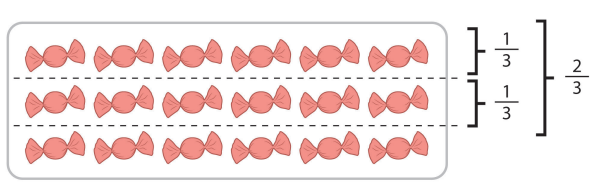
\includegraphics[width=2.9871in,height=1.23958in]{./_SAEB_9_MAT/media/image43.png}
\end{figure}

\num{5} Quando Artur chegou em casa, encontrou uma pizza com alguns pedaços
já consumidos. Como estava com fome, ele também comeu alguns pedaços.
Qual fração de pizza Artur comeu?

\begin{figure}
\centering
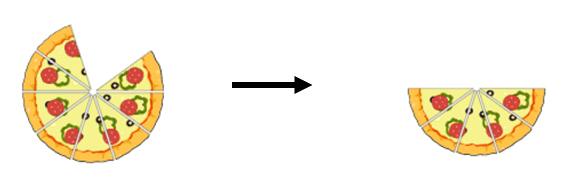
\includegraphics[width=2.75521in,height=0.88894in]{./_SAEB_9_MAT/media/image45.png}
\caption{Uma imagem contendo Seta Descrição gerada automaticamente}
\end{figure}

\reduline{Por meio da imagem, pode-se verificar que, quando Artur chegou em
casa, a pizza ainda tinha 8 pedaços de 10 (porque dois haviam sido 
comidos). Depois de Artur comer, ainda restavam 5 fatias, de
maneira que podemos concluir que Artur consumiu 3, ou seja,
\frac{3}{10}.\hfill}

\num{6} A fração de \frac{2}{7}, ao ser somada com a fração
representada na figura a seguir, será igual a:

\begin{figure}
\centering

\includegraphics[width=1.26562in,height=1.16258in]{./_SAEB_9_MAT/media/image46.png}
\end{figure}

\begin{boxpeq}
\coment{\frac{2}{7} + \frac{5}{8} = \frac{16 + 35}{56} = \frac{51}{56}}
\end{boxpeq}

\num{7} Qual das imagens abaixo representa 4 décimos?

\begin{escolha}
\item
  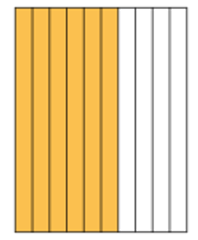
\includegraphics[width=1.0625in,height=1.28788in]{./_SAEB_9_MAT/media/image47.png}

\item
  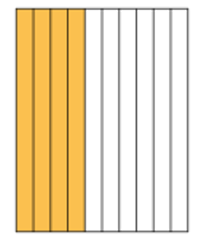
\includegraphics[width=1.07728in,height=1.29167in]{./_SAEB_9_MAT/media/image48.png}

\item
  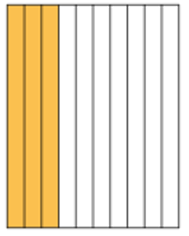
\includegraphics[width=1.00521in,height=1.25518in]{./_SAEB_9_MAT/media/image49.png}

\item
  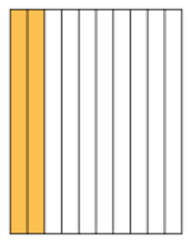
\includegraphics[width=0.9751in,height=1.25in]{./_SAEB_9_MAT/media/image50.png}
\end{escolha}

\begin{boxpeq}
\coment{Observando as imagens apresentadas, verifica-se que todas elas
são divididas em dez colunas. Para obter a proporção solicitada no
enunciado, basta verificar o número de colunas pintadas em relação
ao total de 10.    
a) Incorreta. Nesta alternativa, seis colunas estão pintadas, de modo que
a proporção representada é de \frac{6}{10}. 
a) Correta. Nesta alternativa, quatro colunas estão pintadas, de modo que
a proporção representada é de \frac{4}{10}.
c) Incorreta. Nesta alternativa, três colunas estão pintadas, de modo que
a proporção representada é de \frac{3}{10}.
d) Incorreta. Nesta alternativa, duas colunas estão pintadas, de modo que
a proporção representada é de \frac{2}{10}.}
\end{boxpeq}

\num{8} Considerando o diagrama abaixo, qual fração representa a
quantidade de crianças que preferem hamster como animal de estimação?

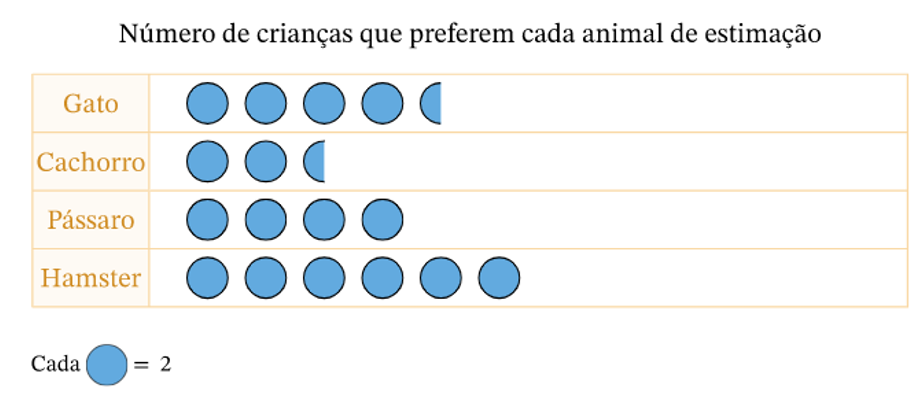
\includegraphics[width=3.85937in,height=1.64922in]{./_SAEB_9_MAT/media/image51.png}

\reduline{Pela contagem, o total de 17 bolinhas representa 34 crianças.
Dessa forma, 12 crianças que preferem hamsters. A fração é \frac{12}{34} = \frac{6}{17}.\hfill}

\num{9} No diagrama abaixo, é possível observar a quantidade de peixes
capturados por Angélica, Pedro, Melissa e Leandro.

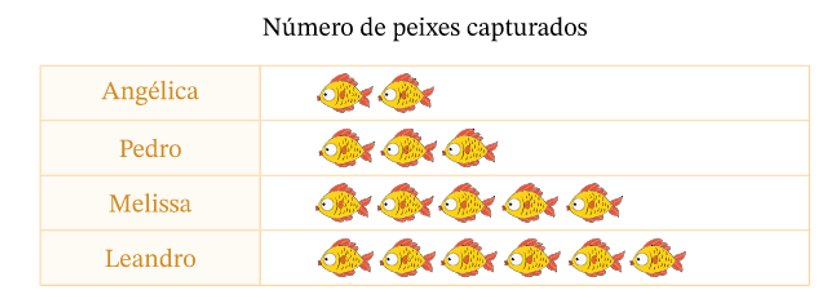
\includegraphics[width=3.65104in,height=1.34767in]{./_SAEB_9_MAT/media/image52.png}

Qual a fração equivalente ao número de peixes do Pedro em relação a
todos?

\begin{boxpeq}
\coment{De acordo com o diagrama, o total de peixes de Angélica, Pedro, 
Melissa e Leandro é de 16. Pedro tem 3 peixes. Dessa forma, a fração da
quantidade de peixes que Pedro tem em relação ao total é
\frac{3}{16}. 
\end{boxpeq}

\num{10} O professor de André montou uma grande lista de exercícios 
e avisou aos alunos que alguns deles iriam cair na avaliação. Alice
já resolveu \frac{4}{5} dos exercícios, Bruno \frac{2}{7}, Augusto 
\frac{12}{15} e Cadu \frac{12}{10}.

Considerando essas informações, quais são os alunos que resolveram a mesma
quantidade de exercícios?

\reduline{Augusto resolveu \frac{12}{15} -- isto é, \frac{4}{5} -- dos 
exercícios. Cadu fez \frac{12}{10}, ou seja,\frac{6}{5}. As frações
equivalentes são, portanto, as de Alice e Augusto.\hfill} 

\section{Treino}

\num{1} A dízima periódica 0,126126... é representada pela fração:

\begin{escolha}

\item \frac{126}{1000}
\item \frac{14}{111}
\item \frac{126}{990}
\item \frac{63}{99}

\end{escolha}

\num{2} O número x, de forma a que as frações \frac{12}{37} = \frac{x}{111} sejam equivalentes, é:

\begin{escolha}

\item 12
\item 24
\item 36
\item 48

\end{escolha}

\num{3} Observando os pedaços de chocolate na imagem a seguir, percebemos 
que há três tipos espalhados: chocolate meio amargo, chocolate ao leite e
chocolate branco. 

\begin{figure}
\centering
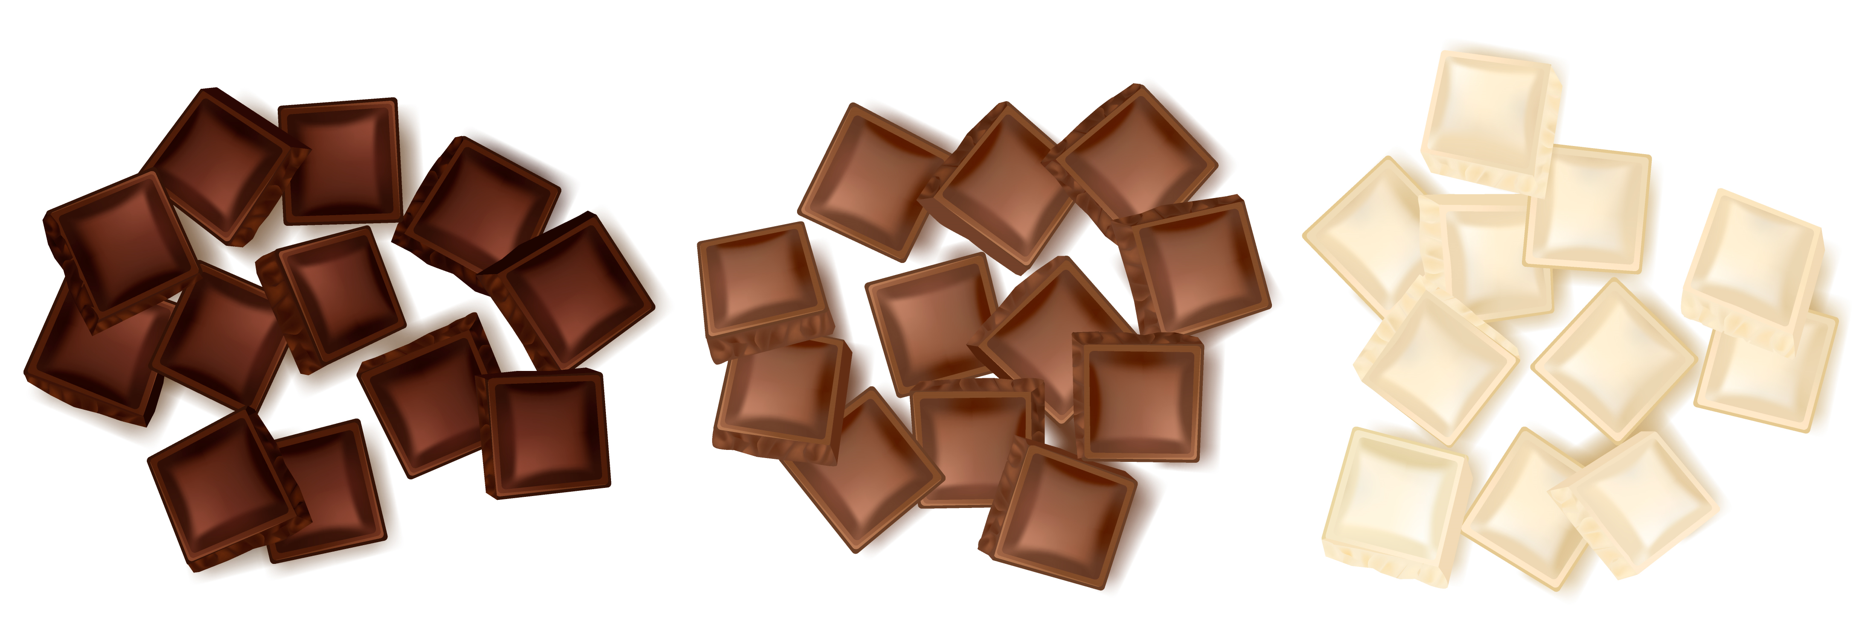
\includegraphics[width=4.54097in,height=1.51544in]{./_SAEB_9_MAT/media/image53.png}
\end{figure}

%\href{https://br.freepik.com/vetores-gratis/conjunto-de-varias-fatias-de-chocolate_10155086.htm\#page=2\&query=chocolate\&position=49\&from_view=search\&track=sph}{Free Vector \textbar{} Vetor grátis conjunto de várias fatias de chocolate (freepik.com)}

Juca comeu \frac{2}{3} do chocolate meio amargo e \frac{1}{2} do
chocolate ao leite.

A fração correspondente à quantidade que Juca comeu em relação ao total é:

\begin{escolha}

\item
  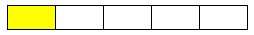
\includegraphics[width=2.11685in,height=0.29169in]{./_SAEB_9_MAT/media/image54.png}
\item
  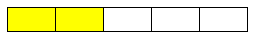
\includegraphics[width=2.10852in,height=0.30003in]{./_SAEB_9_MAT/media/image55.png}
\item
  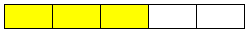
\includegraphics[width=2.08351in,height=0.25002in]{./_SAEB_9_MAT/media/image56.png}
\item
  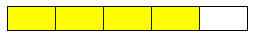
\includegraphics[width=2.10852in,height=0.30003in]{./_SAEB_9_MAT/media/image57.png}
\end{escolha}

\chapter{Porcentagem Aumentos e Descontos}
\markboth{Módulo 4}{}

\section{Habilidades do SAEB}

\begin{itemize}
  \item Resolver problemas que envolvam porcentagens, incluindo os que 
  lidam com acréscimos e decréscimos simples, aplicação de percentuais
  sucessivos e determinação de taxas percentuais.   
\end{itemize} 

\section{Habilidade da BNCC}

\begin{itemize}
  \item EF09MA05.
\end{itemize}

\conteudo{Para determinar aumentos ou descontos sucessivos, utilizamos o 
\textbf{fator de correção}. O fator de correção é dado por F = (1 + i), 
onde i é a taxa percentual de maneira unitária.

Observe os exemplos a seguir.

\begin{itemize}
\item
  3\% = 0,03
\item
  12\% = 0,12
\item
  50\% = 0,5
\end{itemize}

A composição de aumentos e descontos sucessivos pode ser composta por
vários aumentos e vários descontos.

Por exemplo: como calcular o aumento total de um produto que 
passou por dois aumentos sucessivos -- um de 10\% e outro de 15\%?

O percentual total não depende do valor do produto, por isso podemos
fazer:

(1 + 0,1) x (1 + 0,15) = 1,265 $\rightarrow$ 1 + 0,265 , ou seja, um aumento 
de 26,5\% no total.
}

\section{Atividades}

\num{1} Em um período de alta inflação, os itens da cesta básica tiveram
um aumento de 75\%.

Considerando que o preço inicial a cesta básica era de R\$ 60,00, qual
o preço no final do referido período?

\begin{boxpeq}
\coment{Calculando 75\% de 60, teremos 0,75 x 60=45, ou seja, no final
do período teremos o valor de R\$ 105,00}.
\end{boxpeq}

\num{2} Para comprar um tênis no valor de R\$ 250,00, existem duas opções
para pagar, que são as seguintes:

\begin{itemize}
  \item \textbf{Plano I}: Pagamento à vista com 20\% de desconto;

  \item \textbf{Plano II}: Pagamento em duas parcelas iguais sem aumento, a primeira no dia da compra e a segunda um mês depois.
\end{itemize}

Embora o Plano II seja apresentado ao público como vantajoso, o valor
parcelado é mais alto que o do Plano I, pago à vista.

Qual a taxa de juros aplicada no pagamento parcelado?

\begin{largebox}
\coment{O valor do tênis pode até não ser considerado no cálculo, mas, para
facilitar para os estudantes, vamos utilizá-lo.

No Plano I, há desconto de 20\% sobre o valor de R\$ 250,00. Nesse caso,
o valor pago seria de R\$ 200,00, pois seriam dados R\$ 50,00 de desconto.

No Plano II, o comprador tem que desembolsar metade do valor no dia da
compra, ou seja, pagaria no ato R\$ 125,00 e mais R\$ 125,00
após 30 dias, pagando um total de R\$ 250,00. Como, nesse caso,
\textit{as duas parcelas são iguais}, o valor pago em relação ao que 
seria o valor à vista é de \frac{125}{75} = 1,667, ou seja, 66,7\%
a mais. 
}
\end{largebox}

\num{3} Ao longo do ano de 2017 o preço de um artigo esportivo foi
reajustado da seguinte forma: de 15 de março a 15 de abril sofreu um
aumento de 30\%; de 15 de março a 15 de maio, 56\%; de 15 de março a 15
de junho, 48,2\% e de 15 de março a 15 de julho, 90\%.

\begin{figure}
\centering
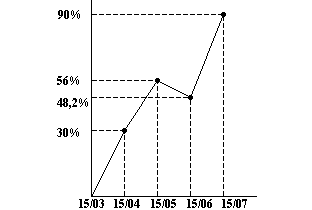
\includegraphics[width=3.25in,height=2.18333in]{./_SAEB_9_MAT/media/image58.png}
\end{figure}

Considerando que o preço em 15/5 era R\$ 120,00, qual foi preço praticado
em 15/7, aproximadamente?

\begin{boxmedio}
\coment{Como em 15/5 o preço estava com 56\% de aumento, podemos retroagir
para o valor em 15/3. Para isso, dividimos 120 por 1,56 e obtemos o valor de
aproximadamente 76,92. Agora podemos fazer o aumento de 90\% que
determinará o valor procurado. Assim: 76,92 x 1,9 = 146,15.}
\end{boxmedio}

\num{4} Observe os valores na tabela. 

\begin{center}
\begin{tabular}{|lll|}
\hline
\multicolumn{1}{|c}{\textbf{Ano}} & \multicolumn{1}{c}{\textbf{Escola A}} & \multicolumn{1}{c|}{\textbf{Escola B}} \\ \hline
\textbf{2022} & R\$ 1000,00 & R\$ 1500,00 \\ \hline
\textbf{2023} & R\$ 1150,00 & R\$ 1680,00 \\ \hline
\end{tabular}
\end{center}

Determine qual escola teve o maior aumento percentual nas mensalidades
de 2022 para 2023 e diga qual foi o percentual de aumento.

\begin{boxmedio}
\coment{Calculando a razão da diferença pelo valor inicial teremos:

Escola A: \frac{150}{1000} = 0,15
Escola B: \frac{180}{1500} = 0,12
O maior aumento foi o da escola A: 15\%.}
\end{boxmedio}

\num{5} O \textbf{Ideb} é o Índice de Desenvolvimento da
Educação Básica e seu objetivo é medir a qualidade do ensino da
educação básica no Brasil.

O gráfico abaixo mostra os resultados do Ideb nacional por biênio de
2005 a 2015.

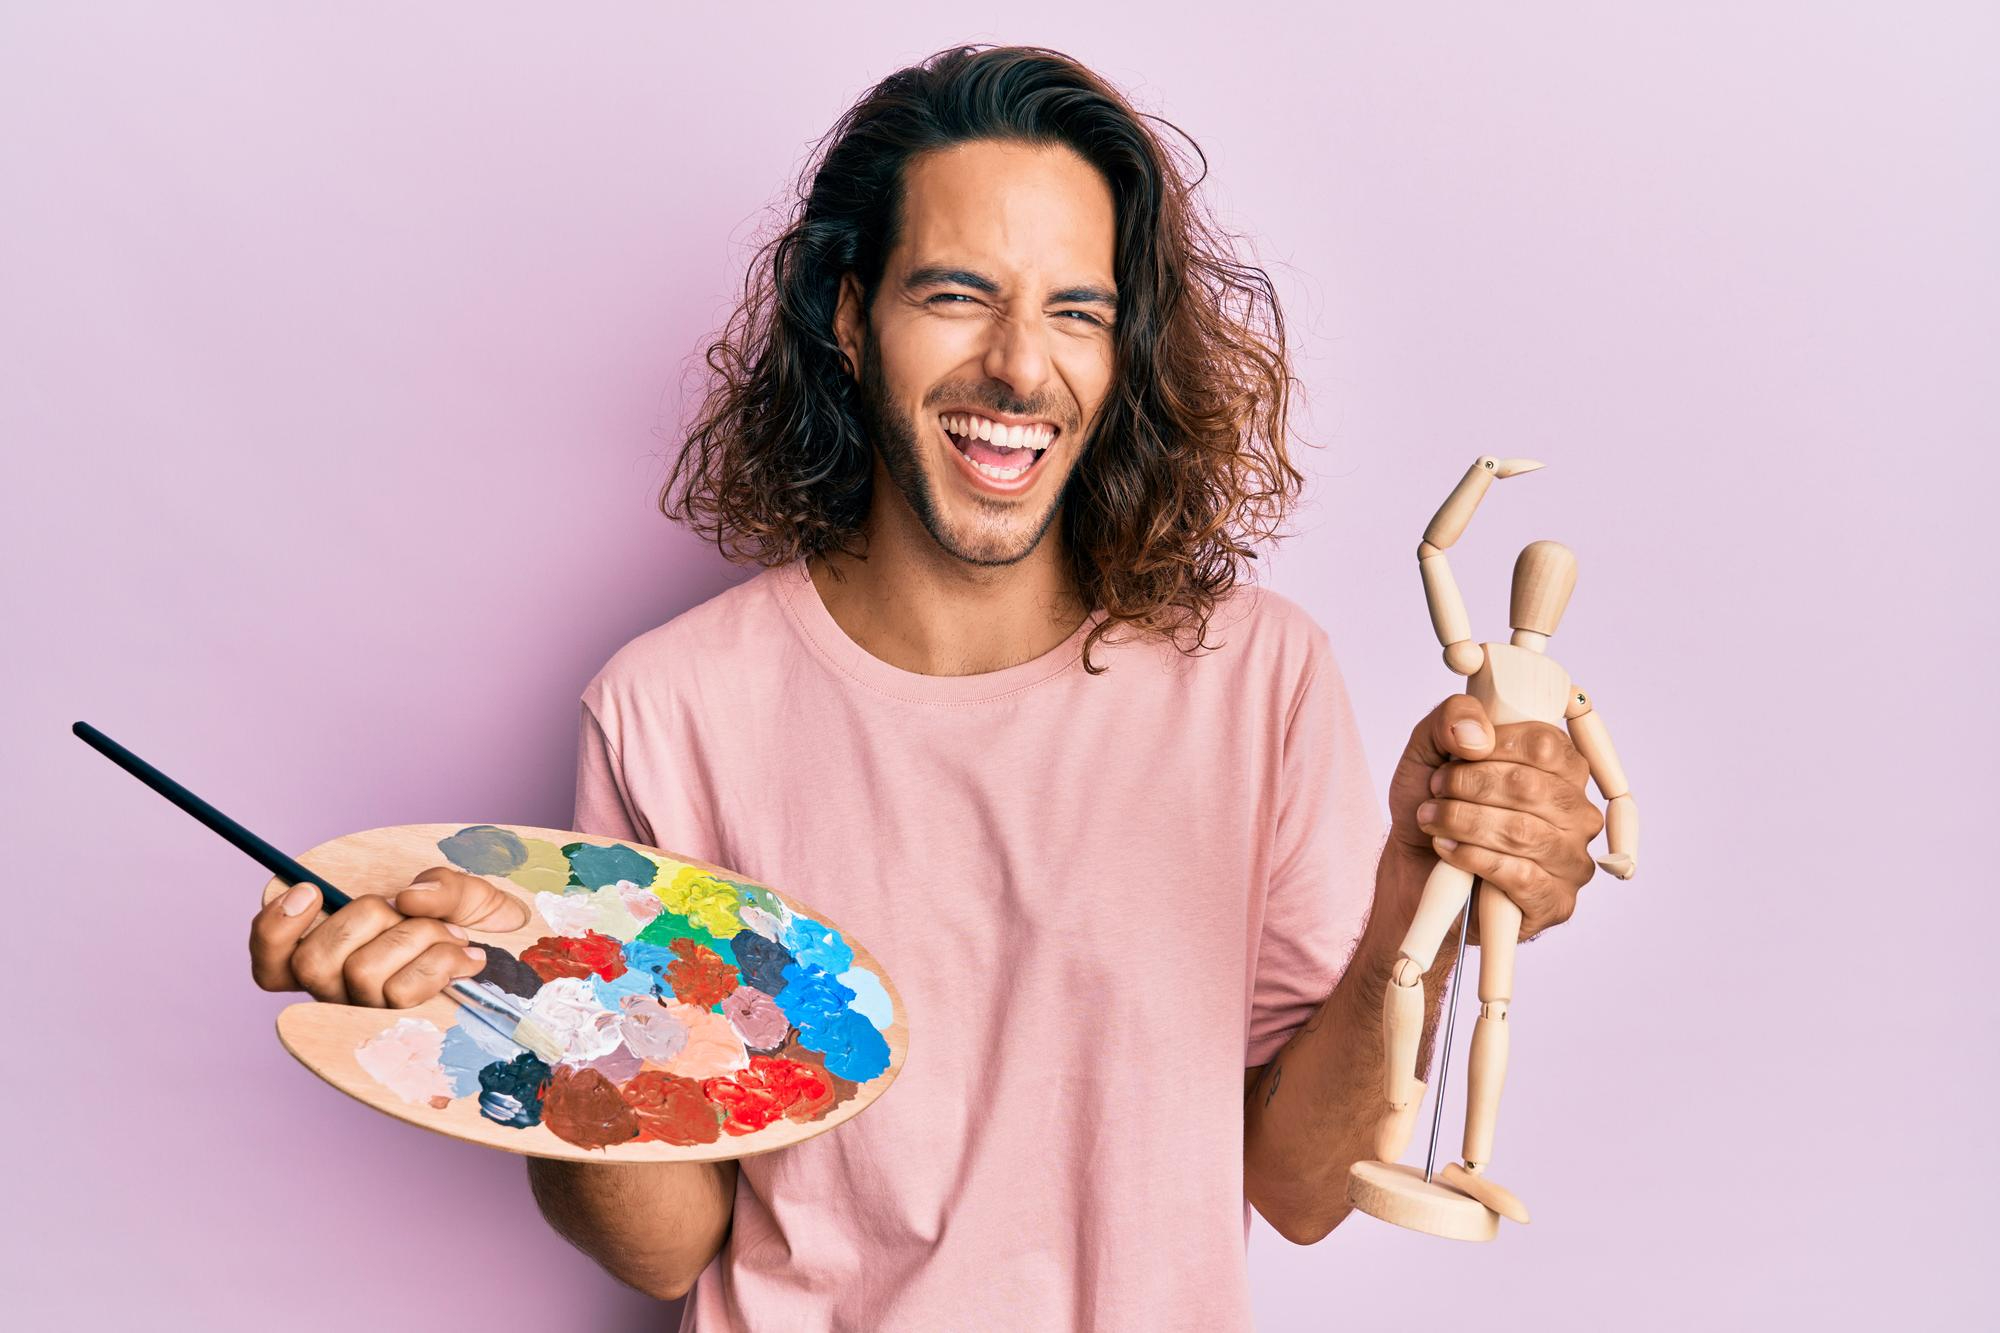
\includegraphics[width=4.91667in,height=2.86449in]{./_SAEB_9_MAT/media/image63.wmf}

No ano de 2021 o índice do Ensino Médio no Brasil foi de 4,2. Qual foi 
o percentual de evolução em relação ao ano de 2015?

\begin{boxpeq}
\coment{O índice era de 3,7 e aumentou para 4,2. Verifica-se, portanto,
um aumento de 0,5 o que representa \frac{0,5}{3,7} \cong 1,1351\ldots\ 
ou seja, um aumento de aproximadamente 13,5\%.}
\end{boxpeq}

\num{6} Leia o texto abaixo para responder à questão.

\begin{quote}
\textbf{Disparidade de rendimento entre sexos permanece alta
apesar do maior ganho para mulheres}

Além da valorização do salário-mínimo, houve aumento real do rendimento
médio de todas as fontes na comparação entre 2010 e 2000. Em 2010, o
rendimento médio era de R\$ 1.587 para os homens e R\$ 1.074 entre as
mulheres.

\fonte{Instituto Brasileiro de Geografia e Estatística. Censo 2010.
Disponível em: https://censo2010.ibge.gov.br/noticias-censo?busca=1&id=1&idnoticia=2747&t=estatisticas-genero-mostram-como-mulheres-vem-ganhando-espaco-realidade-socioeconomica-pais&view=noticia.
Acesso em: 10 mai. 2023.}
\end{quote}

Qual deve ser o desconto sobre o rendimento médio dos homens para
atingir o valor do salário das mulheres?

\begin{boxmedio}
\coment{A diferença entre os salários é 1587 -- 1074 = 513. Calculando a
razão \frac{513}{1587} \cong 0,3232\ldots{}, ou seja, aproximadamente
32,3\%.}
\end{boxmedio}

\num{7} Observe o gráfico a seguir. 

\begin{figure}
\centering
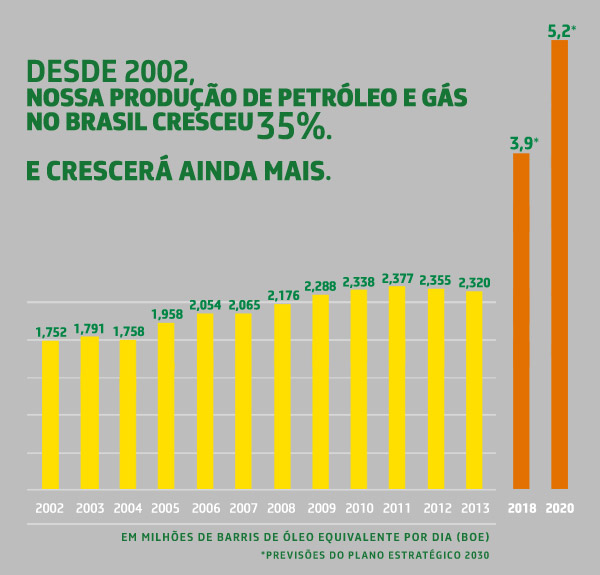
\includegraphics[width=2.91782in,height=2.79636in]{./_SAEB_9_MAT/media/image64.jpg}
\end{figure}

\fonte{Pretrtobras. Disponível em: https://petrobras.com.br/data/files/55/43/0A/53/165954104F528454893851A8/producao-petroleo-VALE-ESTE.jpg. Acesso em: 10 mai. 2023.}

Considerando a previsão realizada em 2013 para atingir a produção de 3,9
milhões de barris por dia, qual deveria ser o percentual de aumento em
relação a 2013?

\begin{boxpeq}
\coment{Calculando a razão \frac{3,9}{2,32} = 1,681\ldots{}. Sendo assim
temos uma previsão de aumento de 68,1\%.}
\end{boxpeq}

\num{8} Calcule o percentual total de aumento sobre um produto que teve
dois aumentos sucessivos de 20\%.

\begin{boxpeq}
\coment{(1 + 0,2) x (1 + 0,2) = 1,44. Assim podemos afirmar que tivemos um
aumento de 44\%.}
\end{boxpeq}

\num{9} Calcule o percentual total de desconto sobre um produto que teve
dois descontos sucessivos de 10\%.

\begin{boxpeq}
\coment{(1 - 0,1) x (1 - 0,1) = 0,81. Assim podemos afirmar que tivemos um
desconto de 19\%.}
\end{boxpeq}

\num{10} Um produto teve um aumento de 20\% e posteriormente um desconto
de 15\%. Considerando o valor final, houve aumento ou desconto? Em que 
porcentagem?

\begin{boxpeq}
\coment{(1 +0,2) x (1 - 0,15) = 1,2 \cdot 0,85 = 1,02. Pode-se afirmar, assim,
que houve aumento de 2\%.}
\end{boxpeq}

\section{Treino}

\num{1} Jorge comprou uma televisão por R\$ 2.150,00 para pagar em duas
parcelas. A primeira parcela corresponde a 30\% do preço da
televisão. O restante foi pago após 30 dias.

Quanto Jorge pagou pela segunda parcela?

\begin{escolha}
\item R\$ 645,00
\item R\$ 1.290,00
\item R\$ 1.505,00
\item R\$ 2.120,00
\end{escolha}


\num{2} Hugo comprou 150 figurinhas para o seu álbum da Copa do Mundo de
2022. Porém, dessas 150 figurinhas, 90 eram repetidas. As figurinhas que
efetivamente foram utilizadas representam qual porcentagem do total de
figurinhas que ele comprou?

\begin{escolha}
\item 40\%
\item 50\%
\item 60\%
\item 90\%
\end{escolha}


\num{3} Kríssia quer comprar à vista uma mochila que custa R\$ 560,00. 
Para pagamento à vista, a loja oferece um desconto de 5\%. Além disso, 
a última peça da loja tembém tem desconto de 20\%.

Ao chegar ao caixa, Kríssia foi surpreendida, pois o desconto de
pagamento à vista foi dado sobre o preço com o desconto de
última peça. Qual foi o valor pago?

\begin{escolha}
\item R\$ 532
\item R\$ 425,60
\item R\$ 420,00
\item R\$ 404,32
\end{escolha}

\chapter{Equação do 1º grau}
\markboth{Módulo 5}{}

\section{Habilidades do SAEB}

\begin{itemize}
  \item Resolver uma equação polinomial de 1o grau.
  \item Inferir uma equação, inequação polinomial de 1o grau ou um sistema de
equações de 1o grau com duas incógnitas que modela um problema.
  \item Associar uma equação polinomial de 1o grau com duas variáveis a uma
reta no plano cartesiano.
  \item Resolver problemas que possam ser representados por sistema de
equações de 1o grau com duas incógnitas. 
\end{itemize} 

\conteudo{\textbf{Equação do primeiro grau} é toda expressão algébrica que
possui incógnita com grau 1. É uma sentença matemática que pode ser
escrita, do tipo ax + b = 0, em que a e b são números reais, e a é
diferente de 0.

O objetivo de escrever uma equação do 1º grau é encontrar qual é o valor
da incógnita que satisfaz a equação. Esse valor é conhecido como 
\textbf{solução} ou \textbf{raiz} da equação.

As incógnitas podem, na definição da equação, ser restritas a um
conjunto numérico cuja raiz seja um elemento. Caso não pertença ao
conjunto universo proposto, dizemos que o conjunto solução é vazio.

O que define o grau de uma equação é o expoente da incógnita. Sendo
assim, quando o expoente da incógnita possui grau 1, temos uma equação
do 1º grau. Observe o exemplo a seguir. 

\begin{itemize}
  
  \item 3x + 5 = 29 (equação do 1º grau com uma incógnita, x)
  
  \item y + 5 = - 3y (equação do 1º grau com uma incógnita, y)
  
  \item 2x -- 3y + 5 = 0 (equação do 1º grau com duas incógnitas, x e y)

\end{itemize}

O maior desafio é ``transformar'' os problemas em uma equação e
resolvê-la. Seguem algumas dicas para resolver problemas
matemáticos em geral:

\begin{itemize}
  \item Leia o problema cuidadosamente: certifique-se de que entende o que
o problema está pedindo. Leia o problema mais de uma vez, se necessário;

  \item Identifique as informações importantes: sublinhe ou destaque as
informações que são relevantes para a resolução do problema. Selecione com
cuidado o que você está tentando encontrar e quais dados você tem;

  \item Desenhe um diagrama: um diagrama pode ajudar a visualizar o
problema e ajudar na solução. Isso pode ser especialmente útil em
problemas geométricos;

  \item Use palavras-chave: muitas vezes as palavras usadas em um
problema podem dar uma indicação de que tipo de operação matemática deve
ser usada. Por exemplo, ``mais'' pode indicar adição, ``menos'' pode
indicar subtração, ``vezes'' pode indicar multiplicação e
``dividido por'' pode indicar divisão;

  \item Escreva equações: transforme as informações importantes do
problema em equações matemáticas. Use variáveis para representar
quantidades desconhecidas;

  \item Simplifique: tente simplificar as equações matemáticas tanto
quanto possível. Isso pode ajudar a reduzir a complexidade do problema;

  \item Resolva a equação: use as propriedades matemáticas para resolver
as equações. Lembre-se de seguir as regras corretas de operações
matemáticas;

  \item Verifique sua resposta: certifique-se de que sua resposta faz
sentido no contexto do problema. Verifique se você respondeu a todas as
partes do problema e se a resposta está em um formato adequado.
\end{itemize}
}

\section{Atividades}

\num{1} Com o objetivo de juntar dinheiro para a formatura, Jorge começou a
produzir doces para revender. Cada receita é composta de \frac{4}{5} kg de 
castanha e \frac{1}{5} kg de açúcar.

Quando Jorge começou a produção, o quilo de castanha custava R\$ 20,00; o do
açúcar, R\$ 4,00. Recentemente, o quilo do açúcar teve aumento e passou a
custar R\$ 4,40. Para manter o custo original com a produção de uma receita, 
Jorge terá que negociar um desconto com o fornecedor de castanha.

Nas condições estabelecidas, o novo valor do quilo de castanha deverá ser
reduzido para qual valor?

\begin{boxmedio}
\voment{Primeiramente calcula-se o custo da receita inicial:

\frac{4}{5} x 20 + \frac{1}{5} x 4 = 16 + 0,8 = R\$ 16,80

Agora vamos calcular o valor da castanha para manter o custo de R\$
16,80.

\frac{4}{5} x X + \frac{1}{5} x 4,4 = R\$ 16,80 \rightarrow
\frac{4}{5} x X + 0,88 = R\$ 16,80 \rightarrow R\$ 19,90.

Portanto, o valor do quilo da castanha deverá ser reduzido para R\$ 19,90.
\end{boxmedio}

\num{2} Um condomínio grande de uma cidade tem três entradas de água. A
vazão de cada entrada é apresentada na tabela a seguir.

\begin{center}
\begin{tabular}{|cc}
\hline
\textbf{Entrada de água} & \multicolumn{1}{c|}{\textbf{Vazão (litro/minuto)}} \\ \hline
\textbf{A} & 50 \\ \hline
\textbf{B} & 60 \\ \hline
\textbf{C} & 90 \\ \hline
\textbf{Vazão total} & 200 \\ \hline
\end{tabular}
\end{center}

Em função do aumento do número de moradores e considerando o histórico
do consumo de água, o síndico do condomínio julgou prudente aumentar em
100\% a vazão total de água nas entradas. Para esse propósito,
as vazões das entradas A e B foram aumentadas ao máximo, para 80 L/min e
100 L/min, respectivamente.

Para que a vazão de água das três entradas juntas seja aumentada em
100\%, em quantos litros por minuto deve ser aumentada a vazão da entrada C?

\begin{largebox}
\coment{A vazão total era de 200 litros por minuto e precisa dobrar. 
Como as entradas A e B passaram a ser de 80 litros por minuto e 100 litros por
minuto, respectivamente, temos:

400 = 80 + 100 + x

220 = x

A entrada C era de 90 L/ min , então 220 -- 90 = 130 L/min, ou seja, um
aumento de 130 L/min.}
\end{largebox}

\num{3} Um vendedor vendeu cadeiras a R\$ 50,00 cada e mesas a R\$ 120,00
cada. No total, o total arrecadado com a venda foi de R\$ 4.800,00. O número 
de cadeiras vendidas é igual a quatro vezes o número de mesas vendidas.

Chamando-se o número de cadeiras vendidas de x e o número de mesas
vendidas de y, crie o sistema que representa, em linguagem
matemática, essa situação e resolva-o.

\begin{boxmedio}
\coment{

\left\begin{matrix}
x = 4y &  & \\ 
50x + 120y = 4800 &  & 
\end{matrix}\right.

50 x 4y + 120y = 4800 \rightarrow y = 15 \therefore x = 60}
\end{boxmedio}


\num{4} Dois lutadores MMA de categorias diferentes foram desafiados para
disputar o cinturão de uma categoria intermediária às suas atuais. Um
deles tinha 91 kg e o outro tinha 77 kg. Eles foram submetidos a uma
intensa jornada de treinos, em que, a cada semana que passava, o primeiro
perdia 1,2 kg, enquanto o outro ganhava 0,6 kg. Logo após esse período de
preparação, a diferença de massa entre os dois atletas era de apenas 4 kg.

Quantas semanas, no mínimo, teve esse período de preparação dos
lutadores?

\begin{boxmedio}
\coment{Lutador A: 91 -- 1,2x
Lutador B: 77 + 0,6x

Lutador A -- Lutador B = 4
(91 -- 1,2x) -- (77 + 0,6x) = 4
91 -- 1,2x -- 77 -- 0,6x = 4
-1,8x = 4 + 77 -- 91
-1,8x = -10
x = 5,56
Passaram-se 5 semanas e 4 dias aproximadamente.}
\end{boxmedio}

\num{5} Marcos pede aos seus pais que tripliquem o valor que recebe de mesada.
Eles aceitam, mas impõem uma condição: reduzir 5 reais do novo valor. Depois 
dessa negociação, fica acordado que Marcos receberá R\$ 60,00. 
Formule a equação que expressa essa situação.

\begin{boxpeq}
\coment{Considerando x como valor inicial da mesada de Marcos, 3x corresponde
ao total que ele pretende receber. Reduzindo-se os R\$ 5,00, o total será
igual a 60, da seguinte maneira: 3x -- 5 = 60.}
\end{boxpeq}

\num{6} Paulo é garçom de um badalado de um restaurante. Ele recebe, por mês,
R\$ 650,00 mais R\$ 20,00 por hora extra que trabalha. Considerando que,
neste mês, ele recebeu um total de R\$ 3150,00, quantas horas extras ele 
trabalhou?

\begin{boxpeq}
\coment{650 + 20x = 3150
20x = 2500
x = 125
Paulo trabalhou 125 horas extras.}
\end{boxpeq}

\num{7} O reservatório de uma chácara estava cheio de água. O proprietário 
da chácara usou \frac{2}{3} desse conteúdo para encher a piscina e, em seguida,
adicionou 3000 litros de água ao reservatório. Com isso, o conteúdo do
reservatório passou a ocupar a metade de sua capacidade inicial. Qual a
capacidade total do reservatório?

\begin{boxmedio}
\coment{ 
\frac{2}{3}x + 3000 = \frac{x}{2}
\frac{x}{6} = 3000
x = 18.000
}
\end{boxmedio}

\num{8} Carol e Alexandre têm, juntos, R\$ 1000. O dobro do
valor de Alexandre corresponde ao triplo do valor de Carol. Qual o valor
que cada um possui?

\begin{boxpeq}

\coment{
  \left\begin{matrix}
C + A = 1000 &  & \\ 
2A = 3C &  & 
\end{matrix}\right.

A = 1000 -- C
2 x (1000 -- C) = 3C
2000 - 2C = 3C
2000 = 5C
C = 400
A = 600
}
\end{boxpeq}

\num{9} Um estacionamento cobra R\$ 8,00 pelas primeiras duas horas e mais
R\$ 1,50 pelas horas subsequentes. Considerando que foram gastos R\$
14,00, qual foi o tempo de permanência?

\begin{boxpeq}

\coment{ 
1,5x + 8 = 14
1,5x = 6
x = 4 horas
}
\end{boxpeq}

\num{10} Nico viaja 350 quilômetros para ir de carro de sua casa à cidade
onde moram seus avós. Em uma dessas viagens, após alguns quilômetros,
ele parou para almoçar. A seguir, percorreu o triplo da quantidade de
quilômetros que havia percorrido antes de parar.

\begin{boxpeq}
\coment{Consideremo o 1º trecho como x. O 2º trecho corresponde ao triplo
de x, ou seja, 3x. Somando os dois, encontra-se o valor de 350.

x + 3x = 350
4x = 350
x = 87,5 km até a parada. 
Depois, Nico percorreu 350 -- 87,5 = 262,5 km.}
\end{boxpeq}

\section{Treino}

\num{1} Aos domingos é comum em algumas cidades termos ciclovias, onde as
famílias inteiras participam de passeios ciclísticos. Uma locadora de bicicleta
cobra R\$ 16,00 por hora de aluguel de uma bicicleta. Além disso,
também cobra uma taxa fixa de manutenção de R\$ 10,00. Carlos alugou uma
bicicleta por 5 horas. Qual o custo ele teve?

\begin{escolha}

  \item R\$ 80,00

  \item R\$ 85,00

  \item R\$ 90,00

  \item R\$ 130,00

\end{escolha}


\num{2} Um estacionamento tem 50 veículos entre carros e motos. Sabendo que o
total de pneus do estacionamento é igual a 160, qual o número de
carros?

\begin{escolha}

  \item 20

  \item 30

  \item 40

  \item 50

\end{enumerate}

\num{3} A soma de três números inteiros consecutivos é 33. Qual é o produto
entre esses três números?

\begin{escolha}
  \item 110

  \item 120

  \item 1320

  \item 4200
\end{escolha}


\chapter{Sequências e Expressões Algébricas}
\markboth{Módulo 6}{}

\section{Habilidades do SAEB}

\begin{itemize}
  \item Identificar uma representação algébrica para o padrão ou a
regularidade de uma sequência de números racionais ou representar
algebricamente o padrão ou a regularidade de uma sequência de
números racionais. 
  \item Identificar representações algébricas equivalentes. 
  \item Resolver problemas que envolvam cálculo do valor numérico de
expressões algébricas. 
\end{itemize} 

\conteudo{\textbf{Sequências numéricas} são conjuntos ordenados de números
que seguem um padrão ou uma regra específica. Essas sequências podem ser 
finitas ou infinitas e podem ser classificadas de diferentes maneiras,
dependendo de suas características.

Algumas das sequências numéricas mais comuns incluem as \textbf{sequências
aritméticas}, que seguem uma regra de adição ou subtração constante entre
seus termos sucessivos, e as \textbf{sequências geométricas}, que seguem uma
regra de multiplicação ou divisão constante entre seus termos
sucessivos.

Outros tipos de sequências numéricas incluem as \textbf{sequências harmônicas},
as \textbf{sequências de Fibonacci} e as \textbf{sequências de números 
primos}. Cada uma dessas sequências tem propriedades e características 
únicas que podem ser estudadas e exploradas por matemáticos e estudantes.

O estudo de sequências numéricas é importante em muitas áreas da
matemática, bem como em outras disciplinas, como física, engenharia e
ciência da computação. As sequências numéricas são usadas para modelar e
descrever fenômenos naturais, para resolver problemas matemáticos e para
desenvolver algoritmos eficientes para uma variedade de aplicativos.

\textbf{Lei de formação}

Há sequências de vários elementos, como meses, nomes, dias da
semana, entre outros. Quando envolve números, a sequência numérica pode
ter uma ``regra'' específica. Podemos formar a sequência de números
pares, números ímpares, números primos, múltiplos de 8 etc.

A sequência numérica pode ser representada por meio de uma \textbf{lei de
formação}. Isso nada mais é que a lista dos elementos da sequência
numérica que seguem a mesma regra. Observe o exemplo a seguir.

Na sequência $a\textsubscript{n}= 3n + 1$, calcula-se o 1º termo com n = 1,
o 2º termo com n=2 e assim sucessivamente. A sequência será 4, 7, 10, 13, 16, 19, \ldots{}

\textbf{Classificação da sequência numérica}

A sequencia numérica pode ser classificada como: crescente, decrescente
ou constante.}

\section{Atividades}

\num{1} Matheus montou figuras com palitos de fósforo. Na 1ª figura, montou
um triângulo e, nas etapas seguintes, foi acrescentando outros triângulos,
conforme se pode observar na imagem a seguir.

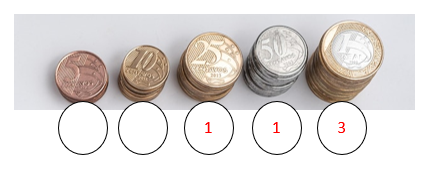
\includegraphics[width=4.44792in,height=1.53053in]{./_SAEB_9_MAT/media/image74.wmf}

Qual a quantidade de palitos de fósforo necessários e suficientes para a
construção da 6ª figura?

\begin{largebox}
\coment{A 1ª figura é composta por 3 palitos; a 2ª figura, por 9; a 3ª,
por 15. Observa-se, portanto, que sempre são acrescentados 6 palitos, 
de modo que uma das expressões que representa a quantidade de palitos é 
$y = 6n -- 3$, onde n é a posição da figura. Para n = 6 teremos: 
$y = 6 x 6 -- 3 = 33$ palitos.}
\end{largebox}

\num{2} Em um grupo de crianças, 210 bombons foram distribuídos
para cada uma, na forma de uma sequência crescente, da criança de menor
estatura para a de maior estatura. Ao colocarmos as crianças nessa
ordem, percebeu-se que a segunda criança ganhou 5 bombons, a quinta
ganhou 11 e sétimo 15. Complete a tabela abaixo para encontrar a
quantidade de bombons de cada criança, desde que sempre seja regular.

\begin{longtable}[]{@{}llllllllll@{}}
\toprule
\textbf{1ª} & \textbf{2ª} & \textbf{3ª} & \textbf{4ª} & \textbf{5ª} &
\textbf{6ª} & \textbf{7ª} & \textbf{8ª} & \textbf{9ª} &
\textbf{10ª}\tabularnewline
\midrule
\endhead
\rosa{3} & 5 & \rosa{7} & \rosa{9} & 11 & \rosa{13} & 15 & \rosa{17} & \rosa{19} & \rosa{21}\tabularnewline
\bottomrule
\end{longtable}

%\coment{A regularidade deve despertar a percepção de que, entre os 2 primeiros números já preenchidos, temos a diferença de 6, mas, ao olhar o 5º e 7º, essa diferença se reduz para 4, ou seja, a mudança de um para outro será de apenas 2 unidades. Não há problemas se os alunos usarem o método de tentativa e erro para resolver a questão.}

\num{3} Observe a quantidade de lugares em cada configuração:

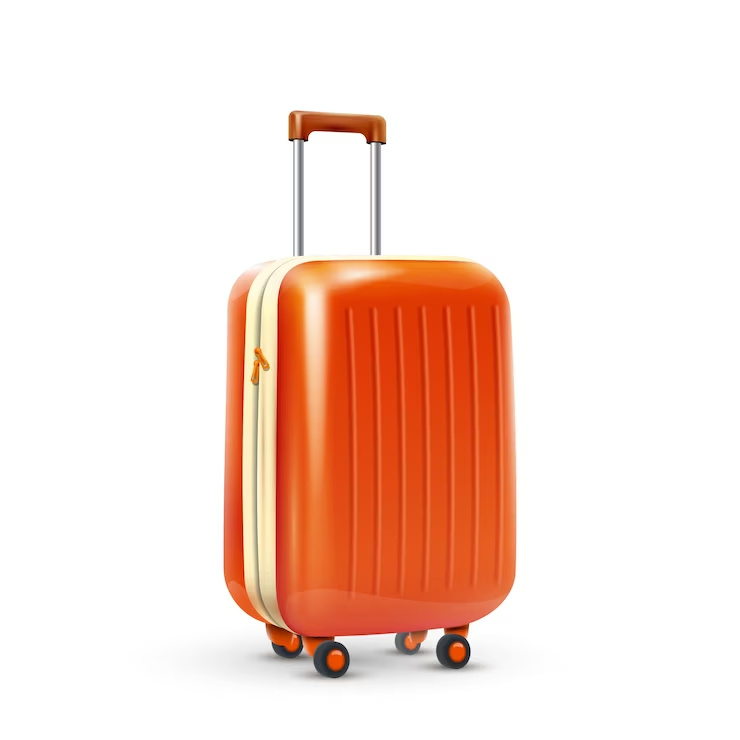
\includegraphics[width=5.72917in,height=1.3in]{./_SAEB_9_MAT/media/image76.wmf}

Se mantivermos o padrão, quantos lugares teremos no total se
acrescentarmos as configurações 4 e 5?

\begin{largebox}
\coment{Na Configuração 1, há 4 lugares; na 2, há 6 lugares que, somados
aos 4 lugares anteriores, resultam em 10; na 3, há 8 lugares que, somados
aos 10 anteriores, completam 18 lugares.

Percebe-se que a próxima configuração a partir da Configuração 3 sempre 
terá duas cadeiras a mais, da seguinte maneira: 4, 6, 8, 10, 12. Essas 
são as quantidades de cadeiras em cada configuração. Somando teremos:
4 + 6 + 8 + 10 + 12 = 40 lugares.}
\end{largebox}

\num{4} Uma fábrica trabalha com vários modelos e tamanhos de mesas. As mesas
são todas acompanhadas com uma certa quantidade de poltronas a depender
do tamanho da mesa.

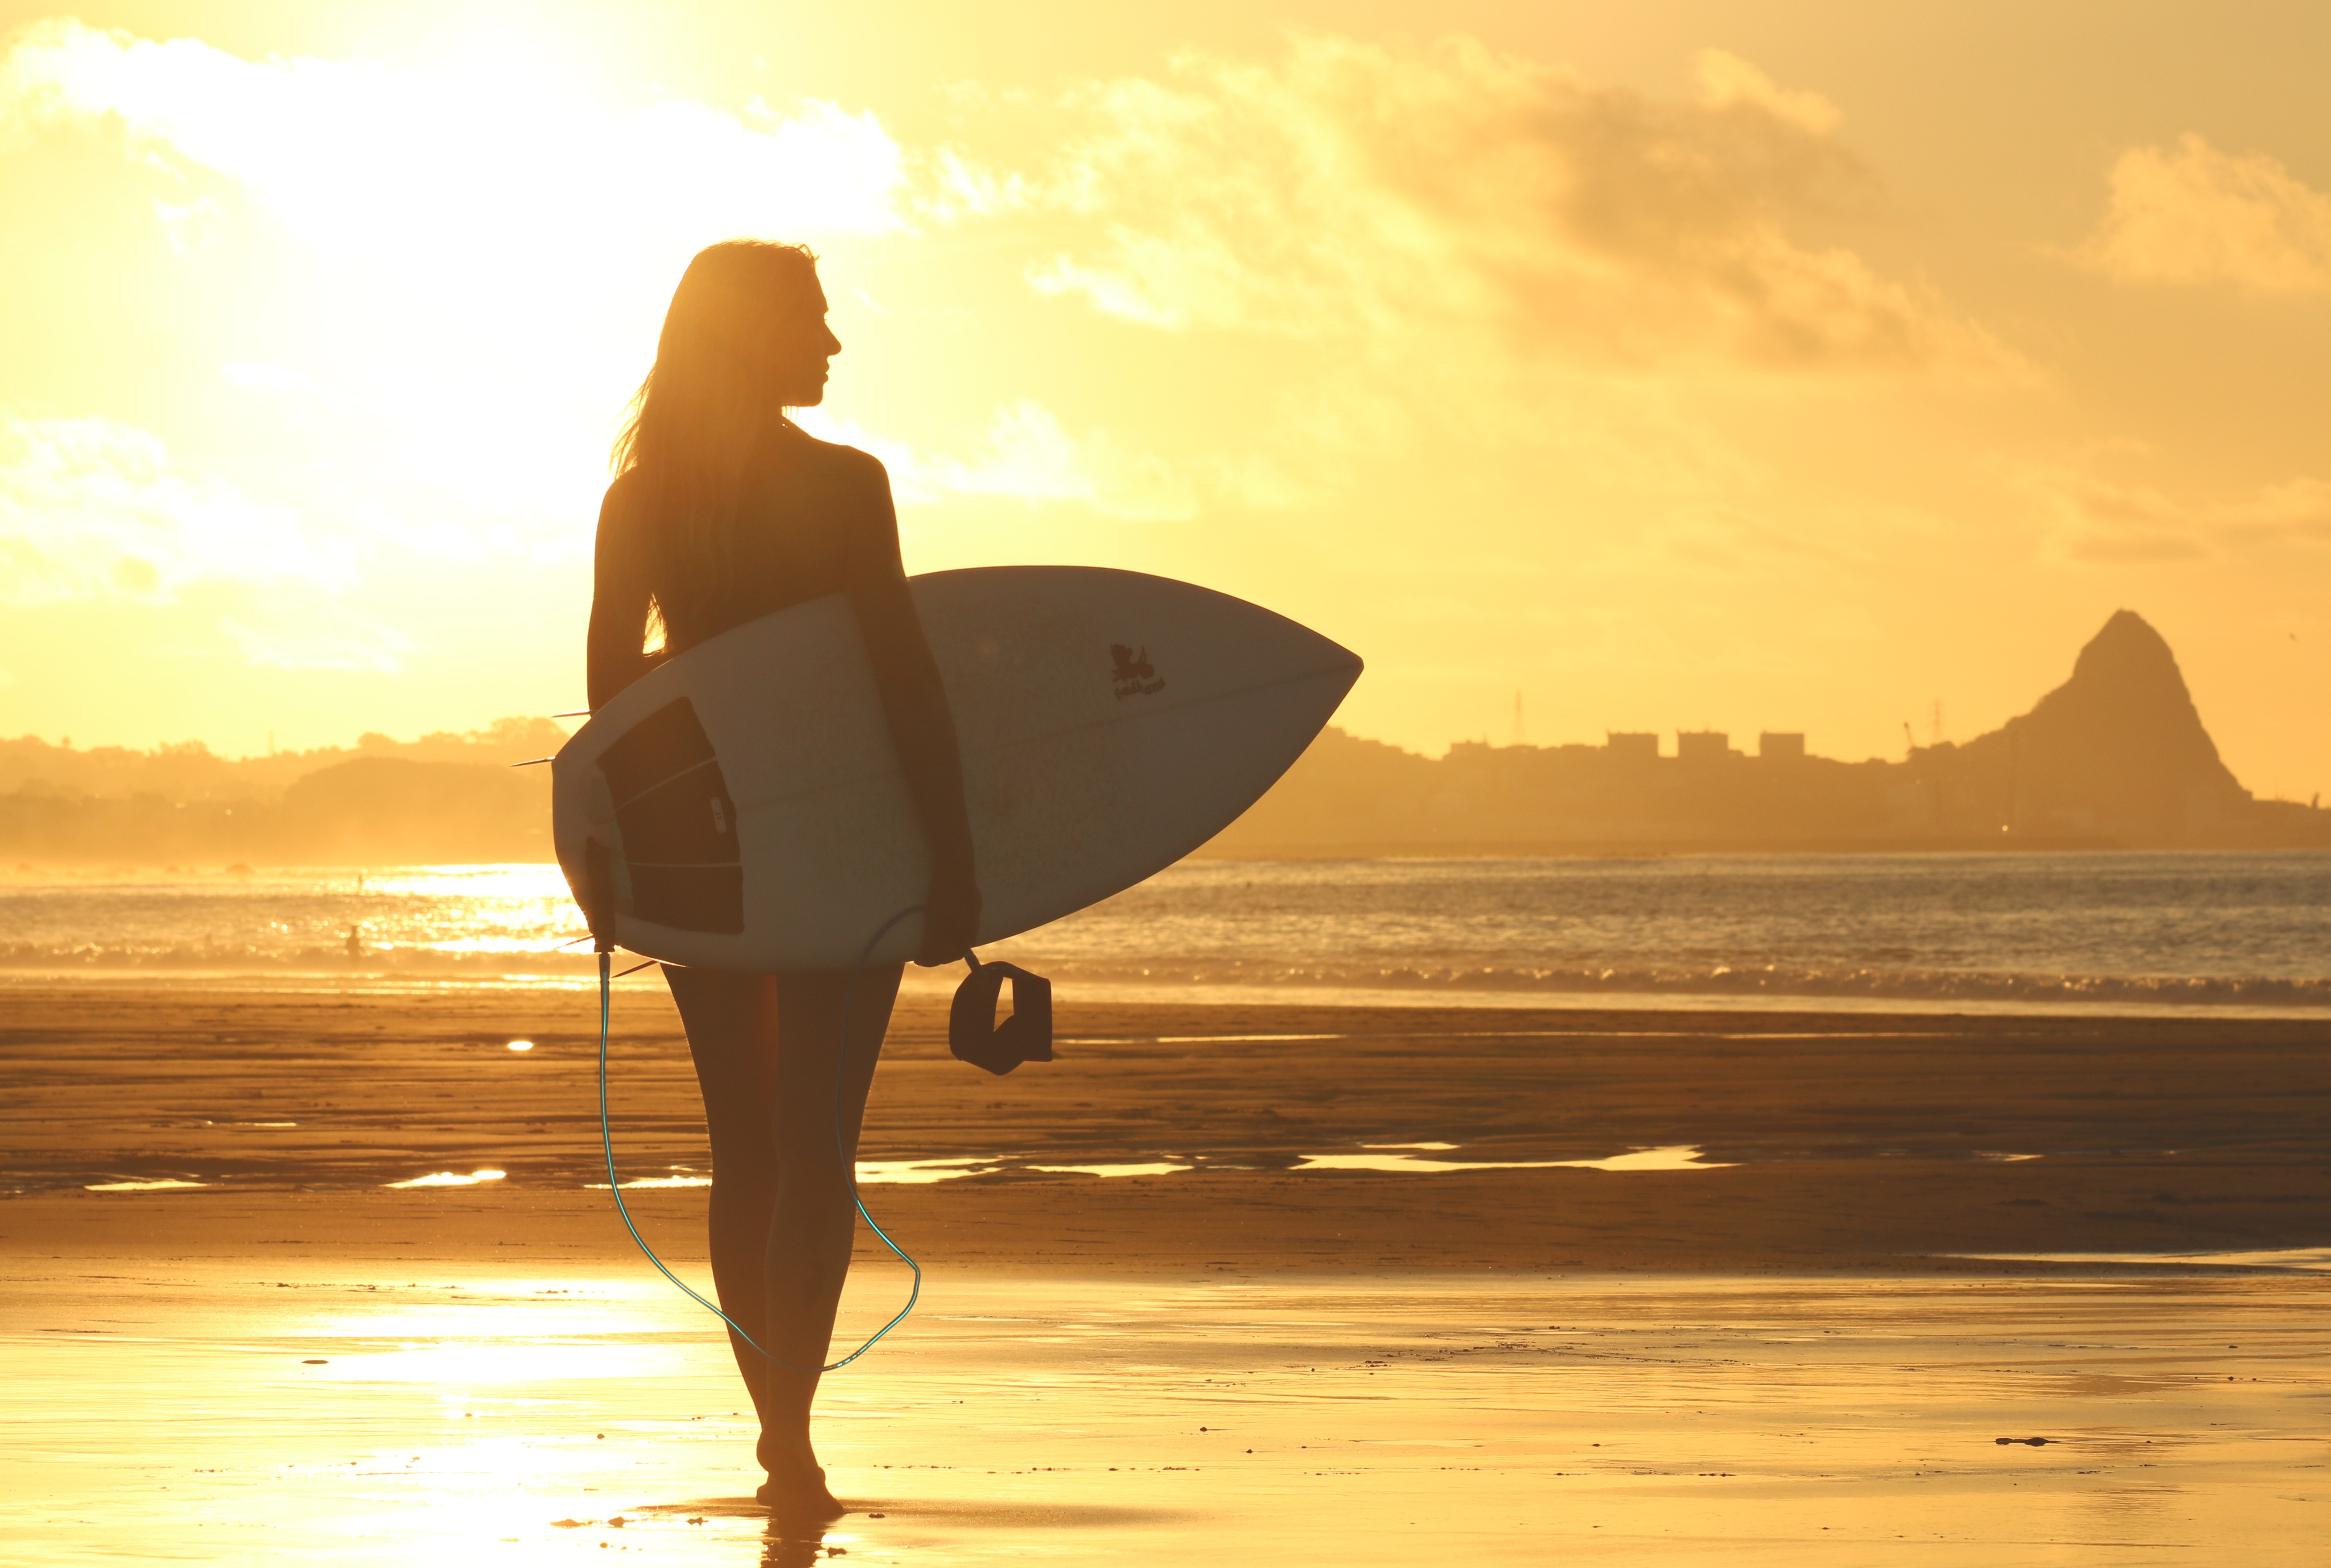
\includegraphics[width=4.28125in,height=1.50833in]{./_SAEB_9_MAT/media/image77.wmf}

O primeiro modelo vem acompanhado de 3 poltronas; o segundo, de 6; o 
terceiro, de 9 poltronas -- e assim sucessivamente. Ao adquirir uma
unidade de cada um dos 10 primeiros modelos de mesa circular, quantas
poltronas estarão disponíveis?

\begin{boxmedio}
\coment{A sequência de poltronas pode ser observada da seguinte maneira:
3, 6, 9, 12, 15, 18, 21, 24, 27, 30. Somando, encontraremos: 3 + 6 + 9 +
12 + 15 + 18 + 21 + 24 + 27 + 30 = 165.}
\end{boxmedio}

\num{5} Felizmente os animais não são mais usados nos espetáculos de circo,
que seguem interessando ao público com outras atrações. Uma delas é a 
\textbf{pirâmide humana}, em que uma pessoa no topo é sustentada por duas
outras, que são sustentadas por mais três, e assim sucessivamente. Quantas
pessoas são necessárias para formar uma pirâmide com 5 linhas de pessoas,
da base ao topo?

\begin{figure}
\centering
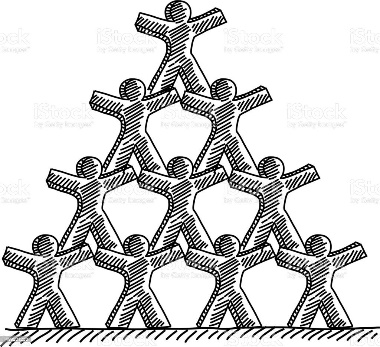
\includegraphics[width=1.71354in,height=1.56302in]{./_SAEB_9_MAT/media/image82.jpeg}
\end{figure}

%\href{https://www.istockphoto.com/pt/vetorial/pir\%C3\%A2mide-criadas-por-pessoas-desenho-gm499201238-79908399?phrase=pir\%C3\%A2mide\%20humana}{Pirâmide Criadas Por Pessoas Desenho - Arte vetorial de stock e mais imagens de Pirâmide Humana - Pirâmide Humana, Esboço, Pirâmide - Estrutura construída - iStock (istockphoto.com)}

\begin{boxpeq}
\coment{Considerando as informações do enunciado e a imagem apresentada, 
quando são usadas 4 linhas, são necessárias 10 pessoas para formar a 
pirâmide. Na próxima linha, haverá mais 5 pessoas, completando um total
de 15.}
\end{boxpeq}

\num{6} Qual o número de cadeiras necessárias ao utilizar 10 mesas na
configuração da imagem abaixo:

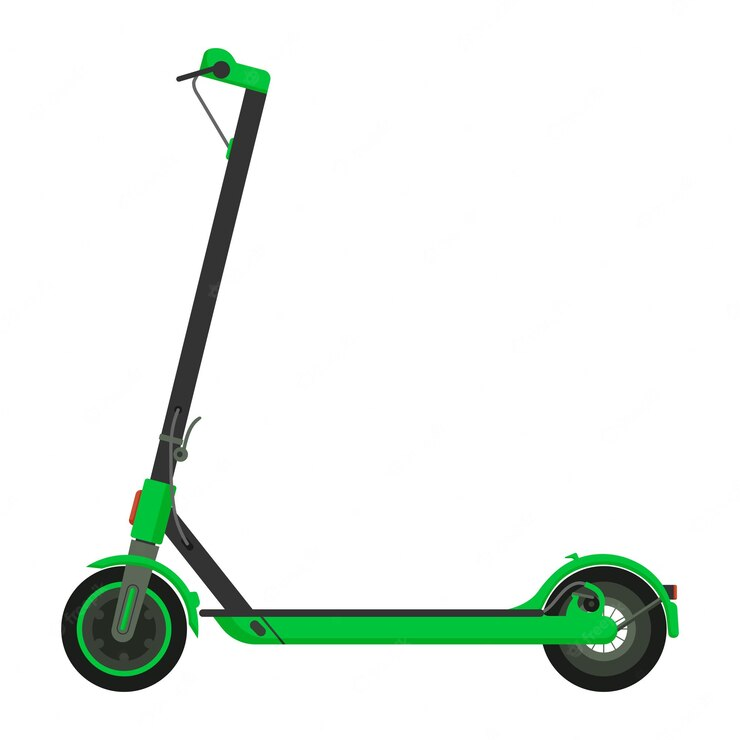
\includegraphics[width=4.6875in,height=0.8in]{./_SAEB_9_MAT/media/image83.wmf}

\begin{boxpeq}
\coment{Considerando a imagem apresentada, observa-se uma sequência numérica
de cadeiras organizada da seguinte forma: 1 mesa, 4 cadeiras; 2 mesas, 6
cadeiras; 3 mesas, 8 cadeiras.
É possível estabelecer uma expressão de quantidade de cadeiras de acordo
com a quantidade de mesas, por exemplo: $y = 2 x n + 2$, com n representando 
a quantidade de mesas. Portanto: $y = 2 \cdot 10 + 2 = 22$ cadeiras.}
\end{boxpeq}

\num{7} Escreva mais 3 números da sequência 18, 30, 42, 54.

\reduline{Para adicionar mais três números à sequência, basta perceber que
a diferença entre 18, 30, 42, 54 é sempre 12 em 12. Portanto, os três
números solicitados são 66, 78, 90.\hfill}

\num{8} Observe a imagem a seguir. 

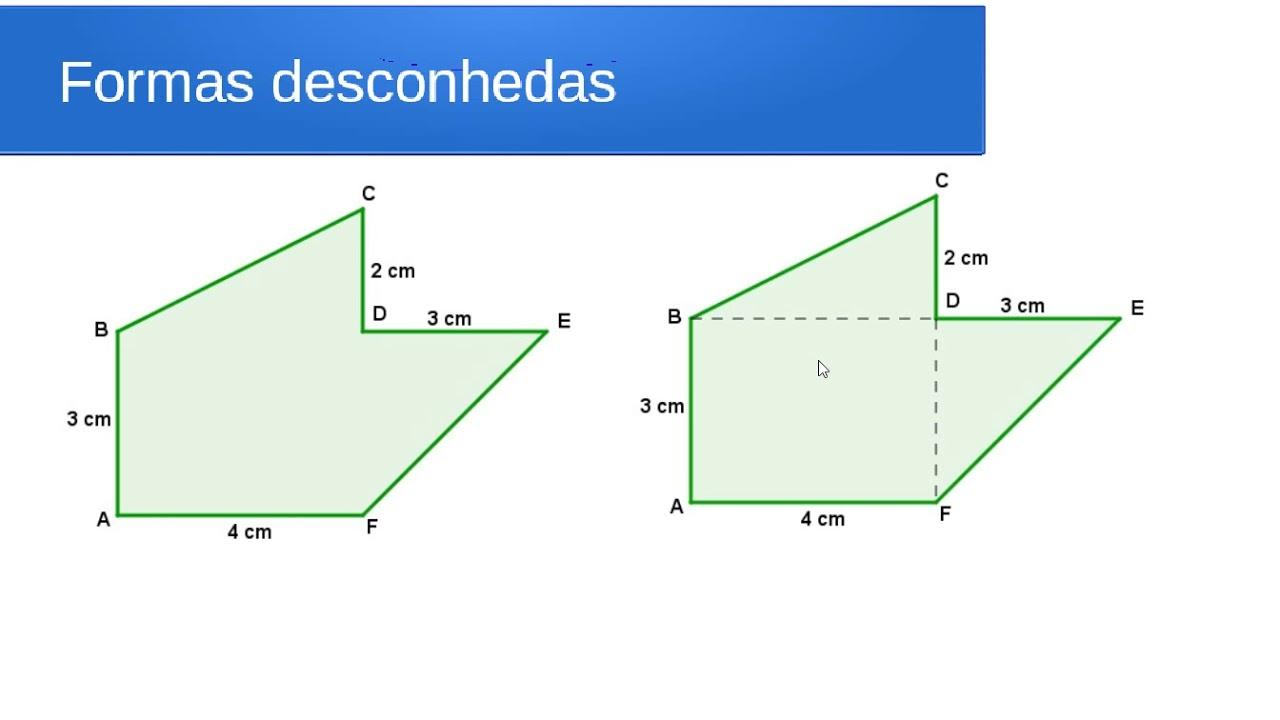
\includegraphics[width=5.68333in,height=1.33333in]{./_SAEB_9_MAT/media/image84.wmf}

Complete a tabela a seguir.

\begin{longtable}[]{@{}lll@{}}
\toprule
Configuração & Número de mesas & Número de lugares\tabularnewline
\midrule
\endhead
1 & \rosa{1} & \rosa{4}\tabularnewline
2 & \rosa{2} & \rosa{6}\tabularnewline
3 & \rosa{3} & \rosa{8}\tabularnewline
4 & \rosa{4} & \rosa{10}\tabularnewline
5 & \rosa{5} & \rosa{12}\tabularnewline
n & \rosa{n} & \rosa{2n + 2}\tabularnewline
\bottomrule
\end{longtable}

\num{9} Qual é a diferença entre o décimo e o quinto termos da sequência 
a\textsubscript{n} = 3n + 2?

\begin{boxpeq}
\coment{$n = 10 32$
$n = 5 17$
$32 -- 17 = 15$}
\end{boxpeq}

\num{10} Observe a sequência: 0, 1, 4, 9, 16, 25, \ldots{}
Qual expressão pode gerar essa sequência?

\begin{boxpeq}
\coment{A sequência é composta pelos quadrados dos números naturais:
$1\textsuperscript{2}$, $2\textsuperscript{2}$, 
$3\textsuperscript{2}$ \ldots{} y = $n\textsuperscript{2}$}
\end{boxpeq}

\section{Treino}

\num{1} Renato colecionou figurinhas da Copa do Mundo. Se ele ganhar mais 8
figurinhas, a quantidade ficará igual ao dobro da quantidade de figurinhas 
que Rodrigo tem menos 12. Se Rodrigo possui 20 figurinhas, então o número de
figurinhas que Renato tem é igual a:

\begin{escolha}

  \item 40

  \item 44

  \item 52

  \item 60

\end{escolha}


\num{2} Caio e Bruna têm, juntos, R\$ 21.000,00 para dar de entrada em um
carro. Caio tem três quartos da quantia de Bruna. Quanto dinheiro Bruna tem?

\begin{escolha}
  \item R\$ 14.200,00

  \item R\$ 13.500,00

  \item R\$ 9.000,00

  \item R\$ 12.000,00
\end{escolha}

\num{3} Um vendedor recebe pagamento composto por uma parte fixa de R\$
850,00 mais um bônus de R\$ 60,00 a cada peça vendida. Se em um
determinado mês ele recebeu o salário de R\$ 1870,00, a
quantidade de produtos vendidos foi igual a:

\begin{escolha}
  \item 15

  \item 16

  \item 17

  \item 18
\end{escolha}

\chapter{Equações do 2º grau}
\markboth{Módulo 7}{}

\section{Habilidades do SAEB}

\begin{itemize}
  \item Inferir uma equação polinomial de 2o grau que modela um problema.
  \item Resolver uma equação polinomial de 2o grau.
  \item Resolver problemas que possam ser representados por equações
polinomiais de 2o grau.   
\end{itemize} 

\section{Habilidade da BNCC}

\begin{itemize}
  \item EF09MA09.
\end{itemize}

\conteudo{
Chamamos de equação do segundo grau as equações do tipo ax² + bx + c = 0
com a, b e c ∈ R, em que \textbf{a} é diferente de zero.

As equações do 2º grau podem ter duas raízes reais iguais, duas raízes
reais distintas ou nenhuma raiz real. O que determina como as raízes são
é o valor encontrado para o discriminante \mathrm{\Delta}.

A maneira mais comum de determinar as raízes da equação do 2º grau é
através da famosa fórmula de Bhaskara:

$\mathrm{\Delta} = b^{2} - 4 x a x c$

$x = \frac{- b \pm \sqrt{\mathrm{\Delta}}}{2 x a}$

Se $\mathrm{\Delta} \textgreater{}0$, então a equação admite duas raízes distintas em
R;

Se $\mathrm{\Delta} = 0$, então a equação admite duas raízes iguais em R;

Se $\mathrm{\Delta} \textless{}0$, ou seja, se $\mathrm{\Delta}$ for 
negativo, a equação não admite solução em R.

As equações do 2º grau podem ser completas ou incompletas. Elas são
incompletas quando o valor referente a \textbf{b} ou \textbf{c} for
ausente, ou seja, igual a zero. Lembrando que o valor de \textbf{a} tem
que ser diferente de zero.

Os parâmetros da equação são:

\begin{enumerate}
  \item \textbf{a} -- coeficiente principal

  \item \textbf{b} -- coeficiente secundário

  \item \textbf{c} -- termo independente
\end{enumerate}

Observe o exemplo a seguir.

\begin{itemize}
\item
  2x\textsuperscript{2} + 6x + 3 = 0 (essa é uma equação do segundo grau)
\item
  Chamamos \textbf{a}, \textbf{b} e \textbf{c} de coeficientes; \textbf{a}
  é sempre coeficiente de \textbf{x²}; \textbf{b} é sempre coeficiente de 
  \textbf{x}; e \textbf{c} é sempre coeficiente do termo independente.
\end{itemize}

Dessa forma:

\begin{enumerate}
\item
  $3x\textsuperscript{2} + 4x + 1 = 0: é uma equação do segundo grau, 
  com a = 3, b = 4, c = 1;
\item
  x² -- x -- 1 = 0: é uma equação incompleta com grau 2, com a = 1, 
  b= --1, c = --1;
\item
  x\textsuperscript{2} -- 5x = 0: também é uma equação incompleta de grau 2, com a = 9, b = --5, c = 0;
\item
  5x\textsuperscript{2} -- 4 = 0: equação do segundo grau, com a = 5, 
  b = 0, c = --4$.
\end{enumerate}
}

\section{Atividades}

\num{1} 

\begin{quote}
O IMC (Índice de Massa Corporal) é um padrão internacional de cálculo
da obesidade de um indivíduo adotado pela OMS (Organização Mundial da
Saúde). O método, desenvolvido pelo belga Lambert Quételet no fim do
século XIX, é a forma mais fácil de saber se uma pessoa está com o peso
ideal ou não.

A altura (calculada em metros) e o peso (calculado em quilogramas) do
indivíduo são os dois fatores levados em conta no cálculo do IMC. Para
calcularmos o índice, basta dividirmos o peso de uma pessoa pela sua
altura ao quadrado.

\fonte{Mundo Educação. IMC. Disponível em: https://mundoeducacao.uol.com.br/saude-bem-estar/imc.htm. Acesso em: 15 mai. 2023}
\end{quote}

A fórmula do \textbf{IMC} é a mesma para todas as pessoas e pode ser
escrita de seguinte maneira:

$h\textsuperscript{2} x IMC - P = 0$

sendo \textbf{h} a altura da pessoa em metros (m) e \textbf{P} o seu peso 
em quilogramas (kg).

Se uma pessoa possui \textbf{IMC} igual a 40kg/m\textsuperscript{2} e está
com peso igual a 120 kg, qual é sua altura?

\begin{boxpeq}
\coment{Substituindo os valores na fórmula dada, chegamos a:

$h\textsuperscript{2} x 40 - 120 = 0 \rightarrow

h = \sqrt{\frac{120}{40}} = \sqrt{3}

\therefore h \cong 1,70m$} 
\end{boxpeq}

\num{2} Calcule os valores das raízes das equações de 2º grau:

\begin{escolha}
  \item $x\textsuperscript{2} + 6x + 8 = 0

  \reduline{Por fatoração podemos escrever a equação $x\textsuperscript{2} + 6x + 8 = (x+4) x (x+2) = 0$.
Com isso, temos como raízes $- 4 e - 2. S={-4, -2}$.\hfill}

  \item x\textsuperscript{2} - 5x - 24 = 0$

  \reduline{Por fatoração podemos escrever a equação $x\textsuperscript{2} - 5x - 24 = 
(x+8)x (x-3) = 0$.
Com isso, temos como raízes $- 8 e 3. S = {- 8, 3}$.\hfill}
\end{escolha}

\begin{boxmedio}
\end{boxmedio}

\num{3} Ao quadrado de um número x você adiciona 7 e obtém sete vezes o
número x, menos 3. Quais são as raízes dessa equação?

\begin{boxpeq}
\coment{$x\textsuperscript{2} + 7 = 7x - 3 \rightarrow

x\textsuperscript{2} -7x + 10 = 0 \rightarrow

(x - 5)\cdot(x - 2) = 0 \rightarrow

x = 5 ou x = 2$}
\end{boxpeq}

\num{4} Suponha que a área de 4.225 km\textsuperscript{2} é delimitada por um
retângulo. Se o comprimento da área excede em sua largura x, formule uma 
equação que permite determinar essa largura x.

\begin{boxpeq}
\coment{Largura x Comprimento

$x \cdot (x + 100) = 4225 \rightarrow

x\textsuperscript{2} + 100x - 4225 = 0$
}
\end{boxpeq}

\num{5} Uma escola pretende colocar o piso das salas de aula como na
figura:

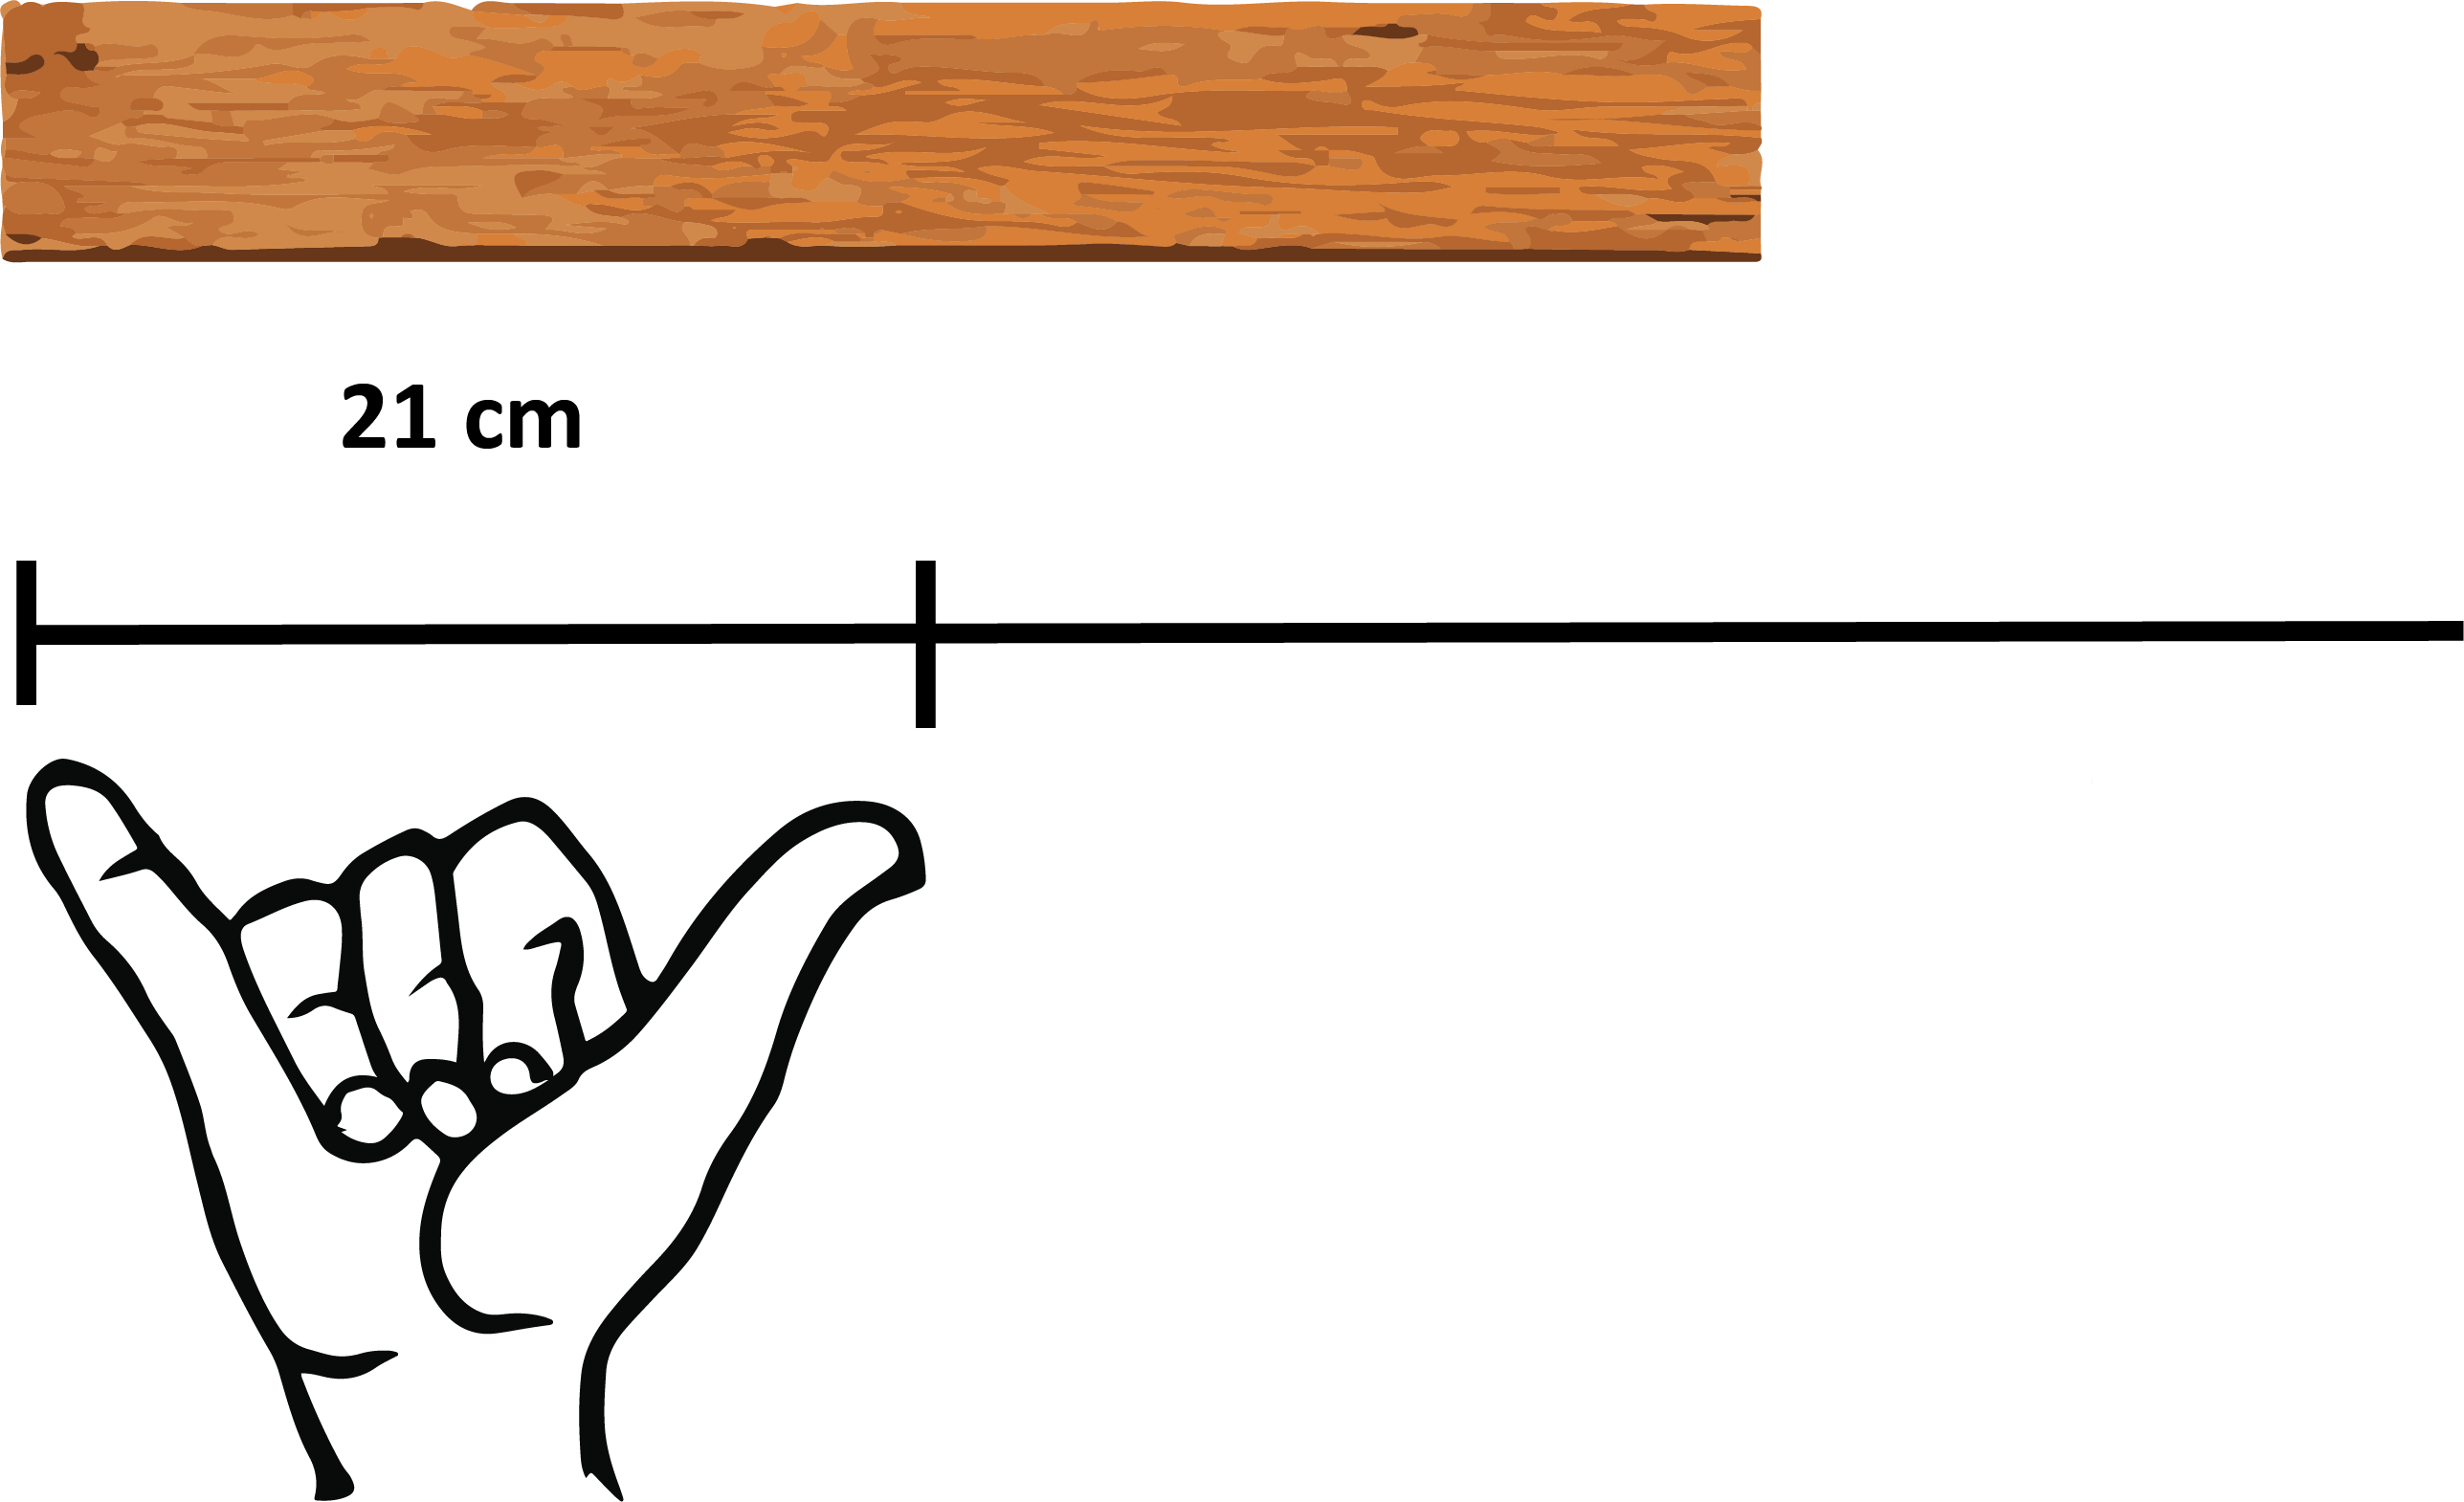
\includegraphics[width=1.70833in,height=1.75833in]{./_SAEB_9_MAT/media/image104.wmf}

Cada piso é formado por quatro retângulos iguais de lados 10 cm e (x +
10) cm respectivamente, e um quadrado de lado igual a x cm.

Sabendo-se que a área de cada piso equivale a 900 cm\textsuperscript{2},
qual é o valor de x, em centímetros?

\begin{boxpeq}
\coment{$4 \cdot 10 \cdot (x+10) + x\textsuperscript{2} = 900 \rightarrow
40x + 400 + x\textsuperscript{2} = 900 \rightarrow
x\textsuperscript{2} + 40x - 500 = 0 \rightarrow
\mathrm{\Delta} = 40\textsuperscript{2} - 4 \cdot 1 \cdot -500 = 3600 \rightarrow
x = \frac{-40\pm\sqrt{3600}}{2\cdot1} \rightarrow$
x = -50 (não convém) ou x = 10}
\end{boxpeq}

\num{6} Um retângulo tem 204\textsuperscript{2}.


\includegraphics[width=2.175in,height=1.29167in]{./_SAEB_9_MAT/media/image107.wmf}

Para uma atividade escolar, precisa-se que o retângulo seja refeito com 3
cm a mais no comprimento e 2 cm a mais na largura e com isso a
superfície aumentou em 76 cm\textsuperscript{2}.

Nessas condições, quais são os dois valores possíveis do comprimento?

\begin{largebox}
\coment{

Do enunciado, temos:
$
\left\begin{matrix}
x \cdot y =204 (i)
\\ (x+3) \cdot (y+2) = 204 + 76 (i)
\end{matrix}\right.
$

Da equação (ii),
$xy + 2x + 3y + 6 = 280$

Como $xy =204$,

$204 + 2x + 3y + 6 = 280 \rightarrow
2x + 3y = 70 \rightarrow
y = \frac{70-2x}{3}$

Substituindo $y = \frac{70-2x}{3}$ na equação (i),

$x \cdot \left ( \frac{70-2x}{3} \right ) = 204

x\textsuperscript{2} - 35x + 306 = 0$

Resolvendo a equação acima, obtemos x = 17 ou x = 18.}
\end{largebox}

\num{7} Um grupo de amigos decidiu alugar uma chácara em um feriado
prolongado para comemorar a formatura. O valor de R\$ 3600,00 seria igualmente
dividido por todos. Devido a alguns problemas financeiros, oito alunos
que estavam no grupo desistiram, e a parte que cada um do grupo deveria
pagar aumentou R\$ 75,00.

Quantos alunos faziam parte do grupo inicialmente?

\begin{largebox}
\coment{Seja x o número de alunos e y o valor de cada aluno, temos 
duas situações:

$\left\begin{matrix}
\frac{3600}{x} = y
\\ \frac{3600}{x-8} = y + 75
\end{matrix}\right.$

Substituindo a primeira equação na segunda, temos:

$\frac{3600}{x-8} = \frac{3600}{x} + 75 \rightarrow
\frac{3600 \cdot x}{x \cdot (x-8)} = \frac{3600 \cdot (x - 8)}{x \cdot (x-8)} + \frac {75 \cdot x \cdot (x - 8)}{x \cdot (x-8)} \rightarrow
3600x - 3600x + 28800 - 75x\textsuperscript{2} + 600x = 0 \rightarrow
- 75x\textsuperscript{2} + 600x + 28800 = 0 (\div 75) \rightarrow
- x\textsuperscript{2} + 8x + 384 = 0$ 

Aplicando soma e produto temos:
$\left\begin{matrix}
x = -16
\\x = 24 
\end{matrix}\right.$

Logo, o total de alunos da turma é 24.}
\end{largebox}

\num{8} Augusto tem 6 anos e Gabriela tem 5. Daqui a quantos anos o produto
de suas idades será igual a 42?

\begin{boxpeq}
\coment{$(x + 6) \cdot (x + 5) = 42
x\textsuperscript{2} + 11x - 12 = 0$
x = - 11 ou x = 1
O produto de suas idades será igual a 42 daqui a 1 ano.}
\end{boxpeq}

\num{9} Um café da manhã que seria dado de presente no valor de R\$ 360,00
deveria ser comprado por um grupo de amigos que contribuíram em partes
iguais. Como 4 deles desistiram, os outros precisaram aumentar a sua
participação em R\$ 15,00 cada um. Qual era a quantidade inicial de 
participantes?

\begin{boxpeq}

\coment{Sendo x igual ao número de rapazes e y igual à quantia que cada um deve
disponibilizar inicialmente, pode-se escrever:

$ xy = 360 \rightarrow y = \frac{360}{x}$

Após a desistência de 4 rapazes, a quantia que cada um deve que
disponibilizar aumentou R\$ 15,00, ou seja:

$(x-4) \cdot (y + 15) = 360 \rightarrow xy - 4y + 15x - 60 = 360$

Sabendo o valor de xy e de y conforme a relação inicial, pode-se
substituir:

$ xy - 4y + 15x - 60 = 360 \\

360 - 4 \cdot \frac{360}{x} + 15x - 60 = 360 \\

- 4 \cdot \frac{360}{x} + 15x - 60 = 0 \\

- 1440 + 15x\textsuperscript{2} - 60x = 0 \\

15x\textsuperscript{2} - 60x - 1440 = 0  \\

x\textsuperscript{2} - 4x - 96 = 0  \\

\Delta = (-4)\textsuperscript{2} - 4 \cdot 1 \cdot (-96) = 400 \\

x = \frac{4 \pm 20}{2}  \\

x_1 = 12 \\

x_2 = - 8 $

Como é impossível ter uma quantidade negativa de pessoas, conclui-se que
o número inicial de rapazes era 12.}
\end{boxpeq}

\num{10} Jandira usou a seguinte frase: ``Um número natural x cujo quadrado
aumentado do seu dobro é igual a 15''. Que número é este?

\begin{boxpeq}
\coment{$x^2 + 2x = 15 \\
x² + 2x -- 15 = 0 $ \\
x = - 5 ou x = 3 
O número é 3.}
\end{boxpeq}

\section{Treino}

%Para mim, essa primeira questão não faz sentido no original. Fiz ajustes. 
\num{1} Em uma empresa, o custo de produção de n peças
iguais é calculado pela seguinte expressão 

$C(n) = n^2 - n + 10$

Se o custo (C) foi de R\$ 82,00, então o número de peças utilizadas
na produção foi

\begin{escolha}
  \item 6

  \item 7

  \item 8

  \item 9
\end{escolha}


\num{2} Eloísa multiplicou a idade atual de seu filho pela idade que ele terá
daqui a 8 anos e obteve como resultado 20 anos.

Qual é a idade atual do filho de Eloisa?

\begin{escolha}
  \item 2 anos

  \item 5 anos

  \item 7 anos

  \item 9 anos
\end{escolha}


\num{3} As idades de dois irmãos são as raízes da equação: 
$x^2 - 24x + 144 = 0$. Com isso, podemos afirmar que:

\begin{escolha}
  \item Eles são gêmeos.

  \item Um deles ainda não nasceu.

  \item Os dois ainda não nasceram.

  \item Um é mais velho do que o outro um ano.
\end{escolha}

\chapter{Grandezas Direta e Inversamente Proporcionais}
\markboth{Módulo 8}{}

\section{Habilidades do SAEB}

\begin{itemize}
  \item Resolver problemas que envolvam variação de proporcionalidade direta
ou inversa entre duas ou mais grandezas, inclusive escalas, divisões
proporcionais e taxa de variação.   
\end{itemize} 

\section{Habilidades da BNCC}

\begin{itemize}
  \item EF09MA07, EF09MA08.
\end{itemize}

\conteudo{
\textbf{Grandeza Diretamente Proporcional}

Dizemos que duas grandezas x e y são diretamente proporcionais quando a
razão (divisão) entre x e y sempre dá o mesmo resultado, ou seja, é
constante.

$\frac{x}{y} = k$

k é a constante de proporcionalidade. Em outras palavras, duas grandezas
são diretamente proporcionais quando uma aumenta e a outra também
aumenta na mesma proporção (quando uma triplica, a outra também
triplica, por exemplo); quando uma diminui, a outra também diminui na
mesma proporção (quando uma cai pela metade, a outra também tem o mesmo
comportamento).

Em nosso cotidiano, a grandeza diretamente proporcional pode ser observada, 
por exemplo, na quantidade de ovos de uma receita: para dobrar a receita,
devemos dobrar também a quantidade de ingredientes. Da mesma forma, uma 
pessoa que recebe apenas pela quantidade de horas trabalhadas, ao triplicar
a quantidade de horas, receberá três vezes mais dinheiro.

Observe, ainda, na tabela a seguir, a relação entre deslocamento e tempo,
com velocidade constante:

\begin{center}
\begin{tabular}{|l|l|l|l|l|l|}
\hline
\textbf{Deslocamento (m)} & 3 & 6 & 9 & 12 & 15 \\ \hline
\textbf{Tempo (s)} & 1 & 2 & 3 & 4 & 5 \\ \hline
\end{tabular}
\end{center}

\textbf{Grandeza Inversamente Proporcional}

Dizemos que duas grandezas x e y são inversamente proporcionais quando o
produto entre x e y é constante.

$x \cdot y = k$

O valor k é denominado constante de proporção.

Em outras palavras, duas grandezas são inversamente proporcionais quando
uma aumenta e a outra diminui na mesma proporção (uma dobra e a outra
cai pela metade, por exemplo).

Um exemplo comum de grandezas inversamente proporcionais é relação
inversa entre velocidade e tempo: quando a velocidade de um carro aumenta, 
o tempo do percurso é reduzido.

Observe a tabela a seguir, na qual o índice de rendimento de produtividade
de cada máquina é o mesmo. Quanto mais máquinas são envolvidas na produção,
menor é o tempo gasto para produzir. 

\begin{center}
\begin{tabular}{|l|l|l|l|l|l|}
\hline
\textbf{Máquinas} & 2 & 4 & 8 & 16 & 32 \\ \hline
\textbf{Tempo (dias)} & 80 & 40 & 20 & 10 & 5 \\ \hline
\end{tabular}
\end{center}
}

\section{Atividades}

\num{1} Uma máquina produz 5 peças a cada 40 segundos. A tabela a seguir
mostra a quantidade de peças que são produzidas por segundo.

\begin{center}
\begin{tabular}{|c ccccc|}
\hline
\textbf{Tempo (segundos)} & 40 & 80 & 120 & 160 & 200 \\ \hline
\textbf{Peças produzidas} & 5 & 10 & 15 & 20 & 25 \\ \hline
\end{tabular}
\end{center}

Depois de 20 minutos, qual a quantidade de peças produzidas?

\begin{boxpeq}
\coment{Em 20 minutos temos $20 \cdot 60 = 1200$ segundos, ou seja, olhando
a tabela pode-se perceber que, se a cada 200 segundos a máquina produz 25 
peças, em 1.200 segundos produzirá $6 \cdot 25 = 150$ peças.}
\end{boxpeq}

\num{2} Uma obra será realizada em uma cidade do interior de São Paulo. A
empresa contratada fez uma planilha com a previsão de todos os gastos
com a execução dessa obra. Foi planejado executar a obra em 16 dias com
25 operários trabalhando 6 horas por dia. Porém, o engenheiro verificou
alguns itens não previstos no projeto fizeram com que a obra tivesse o
triplo da dificuldade inicialmente prevista.

Com o replanejamento, verificou-se que era necessário que o dobro de
operários trabalhasse 8 horas por dia.

Qual o prazo para concluir a obra?

\begin{boxmedio}
\coment{
\begin{tabular}{|c|c|c|c|}
\hline
\textbf{Dias} & \textbf{Horas por dia} & \textbf{Funcionários} & \textbf{Dificuldade} \\ \hline
16 & 6 & 25 & d \\ \hline
x & 8 & 50 & 3d \\ \hline
\end{tabular}

$\frac{16}{x} = \frac{8}{6} \cdot \frac{50}{25} \cdot \frac{d}{3d} \rightarrow \\
\frac{16}{x} = \frac{4}{3} \cdot \frac{2}{1} \cdot \frac{1}{3} \rightarrow \\
\frac{16}{x} = \frac{8}{9} \\
x = 18$

Portanto, o total de dias necessários será 18.}
\end{boxmedio}

\num{3} Uma família que tem sua própria horta sabe que são utilizados 2
litros de água por hora para manutenção da irrigação por gotejamento.
Sabe-se que o reservatório de água tem 20 litros de capacidade. Com essa
quantidade, é possível garantir a irrigação da horta por quantas horas?

\begin{boxpeq}
\coment{Basta calcular a razão $\frac{20}{2} = 10$ horas.}
\end{boxpeq}

\num{4} No período de seca, é comum haver incêndios em matas. Em um destes
incêndios de grandes proporções, foram chamados 60 bombeiros para
realizar o rescaldo numa área de 400 m\textsuperscript{2}. Considerando 
que os bombeiros demoraram 96 horas para controlar as chamas, quantos 
deles teriam sido necessários para controlar as chamas em 50 horas?

\coment{ 
\begin{tabular}{|c|c|c|}
\hline
\rowcolor[HTML]{DAE8FC} 
\textbf{Bombeiros} & \textbf{Área} & \textbf{Tempo} \\ \hline
40 & 400 & 96 \\ \hline
x & 400 & 60 \\ \hline
\end{tabular}

Como a área é fixa, não é necessário considerá-la nos cálculos.

$\frac{40}{x} = \frac{60}{96} \\
x = 64$}

\num{5} Uma pequena fábrica de móveis de madeira tem dois funcionários
especialistas na produção artesanal de uma cadeira de luxo. Lucas
fabrica 20 cadeiras de luxo em 3 dias, trabalhando 4 horas por dia.
Marcel, por sua vez, fabrica 15 cadeiras em 8 dias de 2 horas
de trabalho diário.

A fábrica recebeu uma encomenda de 250 cadeiras. Para atender a essa demanda,
Lucas e Marcel dedicaram 6 horas de trabalho por dia. Quantos dias serão
necessários para entregar as 250 cadeiras?

\begin{boxpeq}
\coment{Lucas fabrica 20 cadeiras em $3 \cdot 4 = 12$ horas; 
Marcel fabrica 15 cadeiras em $8 \cdot 2 = 16$ horas.

O número total de horas necessárias para concluir o trabalho é igual a: $
\frac{250}{\frac{20}{12} + \frac{15}{16}} = \frac{250}{\frac{80 + 45}{48}} = 96$} 
\end{boxpeq}

\num{6} Para administrar um medicamento infantil normalmente a dosagem
depende da massa corpórea da criança. Veja a distribuição da tabela:

\begin{center}
\begin{tabular}{|c|c|}
\hline
\textbf{Massa (kg)} & \textbf{Dosagem (ml)} \\ \hline
Até 5 & 4 \\ \hline
10 & 6 \\ \hline
15 & 9 \\ \hline
\end{tabular}
\end{center}

Seguindo a proporcionalidade, qual deve ser a dose para uma criança de 25
kg?

\begin{boxpeq}
\coment{Pela tabela, verifica-se que a cada 5kg aumenta-se a dosagem em 3 ml, 
de modo que um criança de 25 kg deve tomar 15 ml do medicamento.}
\end{boxpeq}

\num{7} Um comerciante compra maçãs pagando R\$ 7,50 para cada 3 kg e as
revende ao preço de R\$ 30,00 para cada 6 kg. Para que ele obtenha um
lucro de R\$ 420,00 qual quantidade ele deve comprar e revender?

\begin{boxpeq}
\coment{Para 6 kg de maçã o comerciante gasta R\$ 15,00 e recebe R\$ 30,00.
Dessa forma, percebe-se que ele recebe o dobro do valor gasto, de modo que 
seu lucro corresponde à metade valor empregado. Se ele comprar R\$ 420,00 
em maçãs, receberá o mesmo valor em lucro.
$\frac{420}{2,5} = 168$ kg
}
\end{boxpeq}

\num{8} Para calcular seus gastos de transporte e planejar alguma economia,
Fernando coloca no tanque do carro sempre a mesma quantidade de combustível 
e anota o valor gasto. Posteriormente, ele calcula a distância percorrida com
aquela quantidade de combustível e constrói a tabela a seguir:

\begin{tabular}{|l |c|c|}
\hline
\textbf{Combustível} & \cellcolor[HTML]{DAE8FC}\textbf{Valor pago (R\$)} & \cellcolor[HTML]{DAE8FC}\textbf{Distância percorrida (km)} \\ \hline
\textbf{Gasolina comum} & 210 & 350 \\ \hline
\textbf{Gasolina aditivada} & 270 & 360 \\ \hline
\textbf{Etanol} & 175 & 250 \\ \hline
\end{tabular}

Com esses dados, Fernando decidiu verificar o rendimento, ou seja, o custo 
por quilômetro percorrido. Qual foi o combustível mais econômico?

\begin{boxpeq}
\coment{Fazendo as divisões de valor por km temos:

\textbf{Gasolina comum}: 0,60
\textbf{Gasolina aditivada}: 0,75
\textbf{Etanol}: 0,70
O combustível mais econômico foi a gasolina comum.}
\end{boxpeq}

\num{9} Um grupo de cartógrafos decide imprimir um mapa de regiões de
preservação permanente. Eles gostariam que, no mapa, a distância entre
dois pontos seja de 2 cm. Sabendo que a distância real é de,
aproximadamente, 12 km, qual deve ser a escala utilizada no mapa?

\reduline{A razão deverá ser $\frac{2}{12.00000} = \frac{1}{60.0000}$, ou seja,
$1:60.0000$.\hfill}

\num{10} Uma casa de 50 m\textsuperscript{2} de área é construída em 8 dias 
com o trabalho de 10 pessoas. Quantos dias serão necessários para fazer uma 
casa de 80 m\textsuperscript{2} se 15 pessoas trabalharem na sua construção?

\begin{boxmedio}
\coment{Observe a tabela abaixo.

\begin{tabular}{|c|c|c|}
\hline
\textbf{Área} & \textbf{Dias} & \textbf{Pessoas} \\ \hline
50 & 8 & 10 \\ \hline
80 & x & 16 \\ \hline
\end{tabular}

\frac{8}{x} = \frac{50}{80} \cdot \frac{16}{10} \rightarrow \\
\frac{8}{x} = \frac{1}{1} \cdot \frac{2}{2} \rightarrow \\
x = 8$
Portanto, se 15 pessoas trabalharem na construção, serão necessários 8 dias 
para fazer uma casa de 80 m\textsuperscript{2}.}
\end{boxmedio}

\section{Treino}

\num{1} Para abrigar um campeonato de xadrez, seis pessoas trabalharam por 
três dias preparando as salas de aula em que ocorreriam as partidas.

Para que a mesma quantidade total de salas de aula ficasse pronta em um
único dia, quantas pessoas a mais seriam necessárias, trabalhando no mesmo 
ritmo das anteriores?

\begin{escolha}

  \item 18

  \item 15

  \item 12

  \item 8

\end{escolha}

\num{2} Para realizar inscrição em um evento, 3 pessoas atenderam 80 alunos
em 4 horas. Se houvesse 4 pessoas atendendo os alunos no mesmo ritmo, quantas
horas eles levariam para atender 160 alunos?

\begin{escolha}
  \item 3 horas

  \item 5 horas

  \item 6 horas

  \item 8 horas
\end{escolha}

\num{3} Augusto gasta 50 minutos para ir dirigindo de casa ao trabalho com
uma velocidade média de 80 km/h. A uma velocidade média de 50 km/h o tempo
gasto por ele é de aproximadamente:

\begin{escolha}

  \item 10 minutos.

  \item 25 minutos.

  \item 31 minutos.

  \item 64 minutos.

\end{escolha}


\chapter{Função do 1º e 2º grau}
\markboth{Módulo 9}{}

\section{Habilidades do SAEB}

\begin{itemize}
  \item Associar uma das representações de uma função afim ou quadrática a
outra de suas representações (tabular, algébrica, gráfica) ou associar uma
situação que envolva função afim ou quadrática a uma das suas
representações (tabular, algébrica, gráfica).
  \item Resolver problemas que envolvam função afim.  
\end{itemize} 

\section{Habilidade da BNCC}

\begin{itemize}
  \item EF09MA06.
\end{itemize}

\conteudo{A \textbf{função do 1º grau} é uma função linear que pode ser 
escrita na forma $f(x) = ax + b$, onde \textbf{a} e \textbf{b} são constantes
reais. É uma função que representa uma reta no plano cartesiano e tem uma
inclinação constante. Ela é usada para modelar situações que envolvem uma
relação de proporcionalidade direta entre duas variáveis.

Já a \textbf{função do 2º grau} é uma função quadrática que pode ser escrita 
na forma $f(x) = ax^2 + bx + c$, onde \textbf{a}, \textbf{b} e \textbf{c} são
constantes reais, com \textbf{a} diferente de zero. É uma função que
representa uma curva no plano cartesiano e pode ter um ponto máximo ou mínimo.
Ela é usada para modelar situações que envolvem uma relação de 
proporcionalidade indireta entre duas variáveis.

\textbf{Função do 1º grau -- Itens importantes}

\begin{itemize}

  \item $f(x) = ax + b$. O coeficiente \textbf{a} é chamado de \textbf{angular}
  e \textbf{b} de coeficiente \textbf{linear};
  
  \item Seu gráfico é formado por uma reta. Dados dois pontos no plano cartesiano,
  é possível determinar o gráfico da função.
  
  \item A função pode ser \textbf{crescente} ($a\textgreater0$) e 
  \textbf{decrescente} ($a\textless0$).

\end{itemize}

\textbf{Função do 2º grau -- Itens importantes}

\begin{itemize}
  
  \item $f(x) = ax^2 + bx + c$.
  
  \item Seu gráfico é formado por uma parábola. A parábola pode ter concavidade
  para cima ($a\textgreater0$) ou para baixo ($a\textless0$).
  
  \item A função tem \textbf{ponto de máxima} quando a parábola tem a concavidade para baixo e \textbf{ponto de mínimo} quando a parábola tem a
  concavidade para cima.

\end{itemize}
}

\section{Atividades}

\num{1} Uma empresa de transportes calcula o preço a ser cobrado de acordo
com a distância percorrida entre a coleta e a entrega dos objetos. O
preço total a pagar (P) depende da distância (d) a ser percorrida,
acrescido de um valor fixo de R\$ 400,00, referente ao carregamento e à
descarga dos objetos.

Observe os valores na tabela a seguir.

\begin{longtable}[]{@{}lllll@{}}
\toprule
\textbf{Representação parcial do quadro disponível na
empresa}\tabularnewline
\midrule
\endhead
Distância percorrida (km) & 10 & 20 & 30 & ...\tabularnewline
Preço total a pagar (R\$) & 430 & 460 & 490 & ...\tabularnewline
\bottomrule
\end{longtable}

Escreva a função que pode modelar o preço.

\begin{boxpeq}
\coment{Podemos verificar pela tabela que o valor aumenta de 30 em 30 a cada
aumento de 10 km, de modo que o aumento será de 3 em 3 por unidade.

Com isso temos: $P(d) = 3 \cdot d + 400$}
\end{boxpeq}

\num{2} Veja o quadro a seguir e determine a regra matemática que relaciona x
e y.

\begin{tabular}{|c|c|c|c|c|c|c|c|}
\hline
\textbf{x} & - 1 & \rosa{0} & \rosa{1} & 2 & 3 & \rosa{4} & 5 \\ \hline
\textbf{y} & - 4 & \rosa{- 1} & \rosa{2} & 5 & 8 & \rosa{11} & 14 \\ \hline
\end{tabular}

\begin{boxpeq}
\coment{Com a tabela ampliada fica claro o aumento de 3 unidades em y a cada
aumento de 1 unidade em x. Essa regularidade nos aponta que se trata de
função afim do tipo $y = ax+b$ e o valor de a é 3. Para determinar o valor
de b basta ajustar o valor:

Para $x = 0$, por exemplo, $y = 3 \cdot 0 + b = -1$ (dado da tabela) 
$0 + b = -1$, ou seja, $b = - 1$.
$y = 3x - 1$}
\end{boxpeq}

\num{3} Considere o gráfico da função real representado no plano cartesiano a seguir.

\begin{figure}
\centering
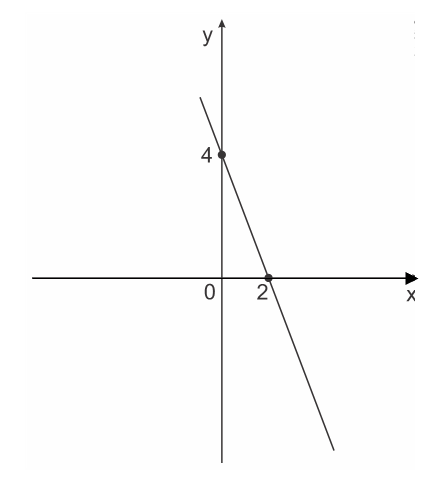
\includegraphics[width=1.97543in,height=2.20513in]{./_SAEB_9_MAT/media/image137.png}
\end{figure}

Determine a função afim, $f(x)$.

\begin{boxmedio}
\coment{Como o eixo y é ``cortado'' no valor 4, temos que $b = 4$. Para
determinar o valor de a, vamos substituir na função, pois pelo gráfico 
sabemos que $f(2) = 0$ (raiz da função).

$f(2) = a \cdot 2 + 4 = 0 \rightarrow \\
2a = - 4 \rightarrow a = - 2 \cdot f(x) = - 2x + 4$.}
\end{boxmedio}

\num{4} Para se deslocar em uma cidade que não possui transporte
de carro por aplicativo, é preciso contar com uma das empresas de transporte.

\begin{tabular}{|l |c|c|}
\hline
 & \textbf{Empresa 1} & \textbf{Empresa 2} \\ \hline
\textbf{Taxa fixa (R\$)} & 5 & 7 \\ \hline
\textbf{Taxa por quilômetro (R\$/km)} & 0,45 & 0,35 \\ \hline
\end{tabular}

Baseado nestes preços, em qual distância o valor das duas 
empresas se iguala?

\begin{boxmedio}
\coment{Empresa 1: $P_1 = 0,45x + 5$

Empresa 2: $P_2 = 0,35x + 7$

$P_1 = P_2 \rightarrow 0,45x + 5 = 0,35x + 7 \\

0,10x = 2 \rightarrow x = 20$ km

Portanto, o valor da corrida das duas empresas é o mesmo quando são 
percorridos 20 km.}
\end{boxmedio}

\num{5} Carlos trabalha como segurança, cobrando uma taxa fixa de R\$ 150,00 mais
R\$ 20,00 por hora. Roberto, na mesma função, cobra uma taxa fixa de R\$ 120,00
mais R\$ 25,00 por hora. Qual é tempo máximo, em horas, para contratarmos Roberto,
de tal forma que não seja mais caro que contratar Carlos?

\begin{boxpeq}

\coment{Carlos: $P_C = 20x + 150$

Roberto: $P_R = 25x + 120$

$P_C = P_R \rightarrow 20x + 150 = 25x + 120 \\

30 = 5x \rightarrow  x = 6$.}
\end{boxpeq}

\num{6} O corte transversal de um túnel, de pista única, tem base de 30 m de largura
e altura máxima de 10 m. O formato é um arco de parábola, conforme representado na
ilustração e no gráfico a seguir, sendo V o vértice da parábola.

\begin{figure}
\centering
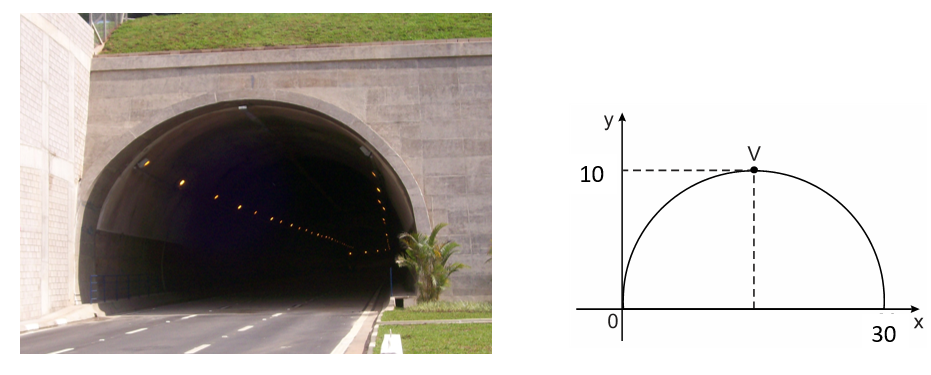
\includegraphics[width=5.56667in,height=2.24198in]{./_SAEB_9_MAT/media/image143.png}
\end{figure}

Escreva uma função que modele essa parábola.

\begin{largebox}
\coment{$f(x) = a \cdot (x - x_1) \cdot (x - x_2)$,
considerando $x_1 = 0$ e $x_2 = 30$ 

Temos então:

$f(x) = a \cdot (x - 0) \cdot (x - 30) = a \cdot (x^2 - 30x)$. 

Como a parábola é simétrica, a altura é determinada quando $x = 15$.

$ f(15) = a \cdot (15^2 - 30 \cdot 15) = 10 \\

a \cdot (225 - 450) = 10 \rightarrow a = - \frac{10}{225} =  - \frac{2}{45} \\

f (a) = - \frac{2}{45} (x^{2} - 30x)$.}
\end{largebox}

\num{7} Em uma indústria, o custo de produção em mil reais de x mil unidades
de determinado produto é dada pela função $ C(x) = 0,1^2 - 4x + 70$. Calcule 
o custo para a produção de 100 unidades.

\reduline{Calculando o custo para $x = 100$ temos:

$C(100) = 0,1 \cdot (100)^2 - 4 \cdot 100 + 70 = 0,1 \cdot 10000 - 400 + 70 = 670$.\hfill}

\num{8} A concentração de um medicamento C de certa medicação, em mg/l, varia de
acordo com a função $C = 6t - \frac{1}{4} t^2$ em que t é o tempo decorrido, em 
horas, após a ingestão da medicação, durante um período de observação de 24 horas.
Determine a concentração após 12 horas.

\begin{boxpeq}
\coment{$C = 6 \cdot 12 - 0,25 \cdot 12^2 = 72 - 36 = 36$.}
\end{boxpeq}

\num{9} Qual função representa o gráfico abaixo?

\begin{figure}
\centering
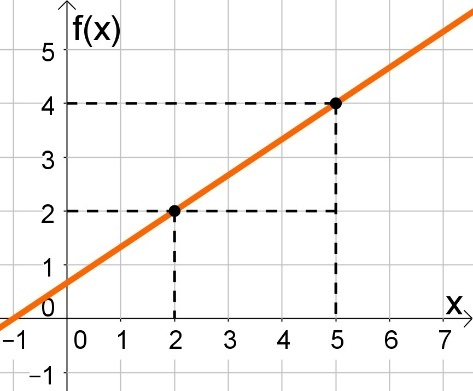
\includegraphics[width=2.14105in,height=1.76667in]{./_SAEB_9_MAT/media/image150.jpeg}
\end{figure}

\begin{largebox}
\coment{Sabemos que $f(2) = 2$ e $f(5) = 4$. Dado o gráfico sabemos que a função é
do tipo $f(x)=ax+b$.

$f(2)=2a + b = 2 \\

f(5)=5a + b = 4$

Resolvendo o sistema:

$\left\begin{matrix}
2a + b = 2
\\5a + b = 4 
\end{matrix}\right. \rightarrow 3a = 2 \rightarrow a = \frac{2}{3} \\

5 \cdot \frac{2}{3} + b = 4 \rightarrow \frac{10}{3} - 4 = - b \\

b = \frac{2}{3} \\

f(x) = \frac{2}{3}x + \frac{2}{3}$.
}
\end{largebox}

\num{10} O deslocamento de um balão é dado pelo gráfico abaixo. Sabe-se que a
altura máxima foi atingida na metade do tempo. A altura h em metros, do
balão, está em função do tempo t em horas, por meio da fórmula 
$h(t) = - \frac{3}{4} t^2 + 6t$. Qual é altura máxima?

\begin{figure}
\centering
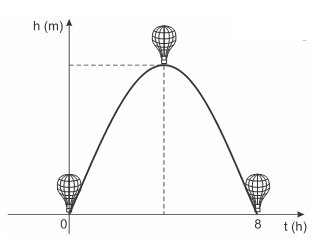
\includegraphics[width=2.62523in,height=2.05851in]{./_SAEB_9_MAT/media/image154.png}
\end{figure}

\begin{boxpeq}
\coment{A altura máxima foi atingida no tempo de 4 horas, de modo que:

$ h(4) = - \frac{3}{4}4^{2} + 6 \cdot 4 = - 12 + 24 = 12$ horas.}
\end{boxpeq}

\section{Treino}

\num{1} Uma prestadora de serviços cobra pela visita à residência do
cliente e pelo tempo necessário para realizar o serviço na residência. O
valor da visita é R\$ 60,00 e o valor da hora para realização do serviço é
R\$ 35,00. Uma expressão que indica o valor a ser pago (P) em função das
horas (h) necessárias à execução do serviço é:

\begin{escolha}
  \item P = 40h

  \item P = 60h

  \item P = 35 + 60h

  \item P = 60 + 35h
\end{escolha}

\num{2} Uma aplicação financeira tem valorização determinada pelo gráfico abaixo.
Considerando os dados apresentados, determine o valor no tempo de 10 anos.

\begin{figure}
\centering
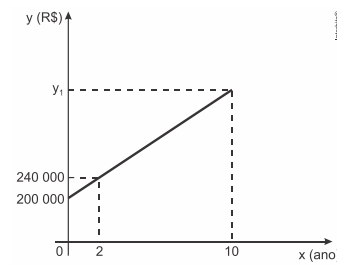
\includegraphics[width=2.80858in,height=2.3252in]{./_SAEB_9_MAT/media/image155.png}
\end{figure}

\begin{escolha}
\item R\$ 260.000,00

\item R\$ 300.000,00

\item R\$ 320.000,00

\item R\$ 400.000,00
\end{escolha}

\num{3} Observe o gráfico apresentado abaixo:

\begin{figure}
\centering
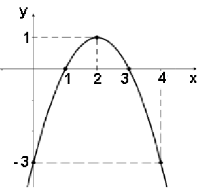
\includegraphics[width=1.72515in,height=1.5668in]{./_SAEB_9_MAT/media/image156.png}
\end{figure}

Qual é o ponto de máximo?

\begin{escolha}

\item (1,0)

\item (2,1)

\item (3,0)

\item (4,-3)

\end{escolha}

\chapter{Geometria Plana I}
\markboth{Módulo 10}{}

\section{Habilidades do SAEB}

\begin{itemize}
  \item Identificar, no plano cartesiano, figuras obtidas por uma ou mais
transformações geométricas (reflexão, translação, rotação).
  \item Relacionar o número de vértices, faces ou arestas de prismas ou
pirâmides, em função do seu polígono da base.
  \item Relacionar objetos tridimensionais às suas planificações ou vistas.
  \item Classificar polígonos em regulares e não regulares.
  \item Reconhecer polígonos semelhantes ou as relações existentes entre
ângulos e lados correspondentes nesses tipos de polígonos.
  \item Reconhecer circunferência/círculo como lugares geométricos, seus
elementos (centro, raio, diâmetro, corda, arco, ângulo central, ângulo
inscrito).
  \item Construir/desenhar figuras geométricas planas ou espaciais que
satisfaçam condições dadas.
  \item Resolver problemas que envolvam relações entre os elementos de uma
circunferência/círculo (raio, diâmetro, corda, arco, ângulo central, ângulo
inscrito).
\end{itemize} 

\section{Habilidades da BNCC}

\begin{itemize}
  \item EF09MA11, EF09MA12.
\end{itemize}

\conteudo{
\begin{itemize}
  \item \textbf{Plano Cartesiano}
\end{itemize}

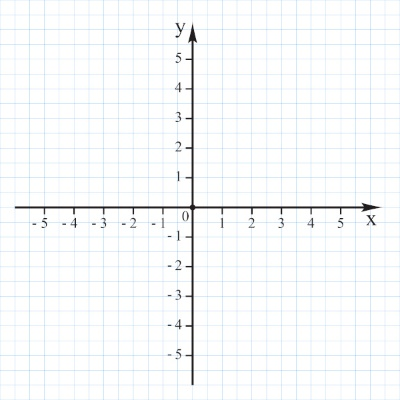
\includegraphics[width=1.8125in,height=1.8125in]{./_SAEB_9_MAT/media/image157.jpeg}

O plano cartesiano tem os pontos indicado par ordenado (a, b). O valor
\textbf{a} é a abscissa e \textbf{b} é a ordenada. Por exemplo, o ponto
A é (2,3).

\begin{itemize}
  \item \textbf{Polígonos}
\end{itemize}  

Polígonos são formas geométricas planas compostas por segmentos de reta
que se unem em vértices. Eles são classificados como convexos ou
não convexos.

Observe os exemplos de polígonos convexo e não convexo.

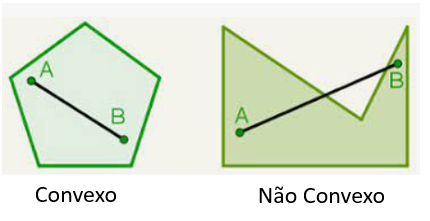
\includegraphics[width=2.32292in,height=1.19387in]{./_SAEB_9_MAT/media/image160.png}

O polígono será convexo quando o segmento de reta determinado por dois pontos A e B
quaisquer estiver inteiramente contido no interior do polígono. 

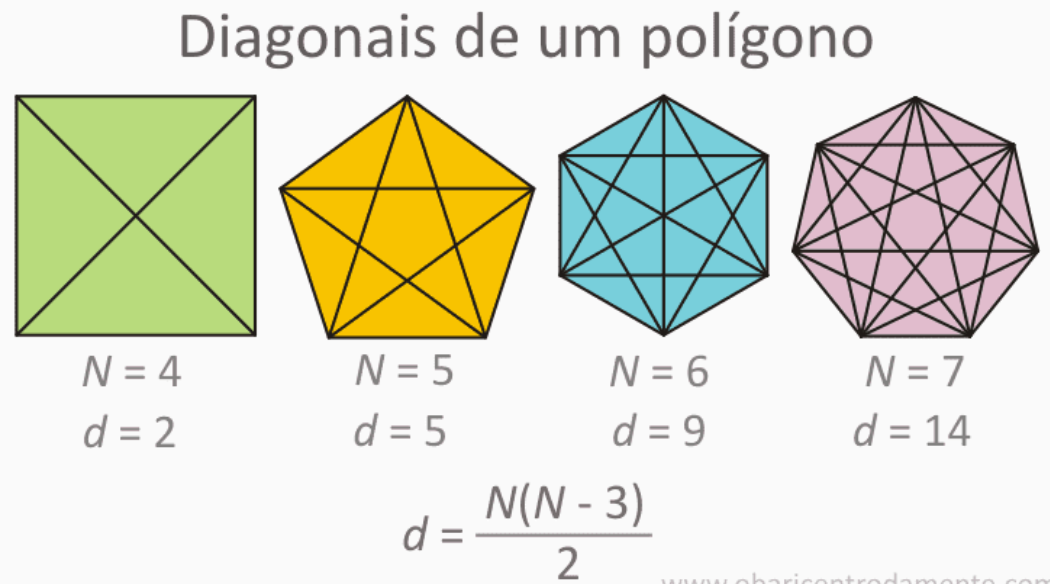
\includegraphics[width=3.07204in,height=1.70833in]{./_SAEB_9_MAT/media/image161.png}

\begin{itemize}
  \item \textbf{Relações de Euler}
\end{itemize}

A relação de Euler nos ajuda a definir a quantidade de vértices, arestas
e faces.

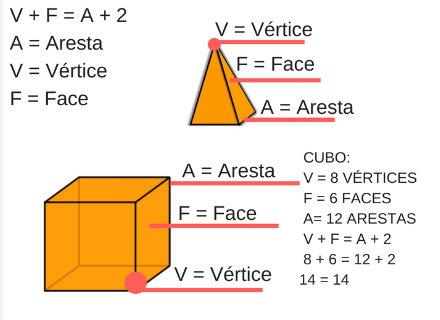
\includegraphics[width=3.61979in,height=2.66667in]{./_SAEB_9_MAT/media/image162.png}

\begin{itemize}
  \item \textbf{Elementos da circunferência}
\end{itemize}

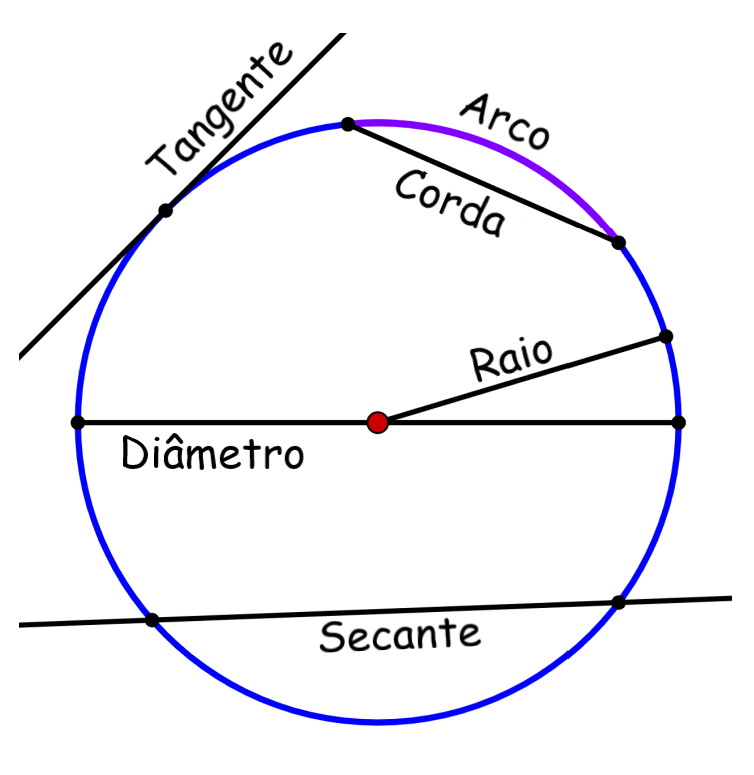
\includegraphics[width=1.53027in,height=1.57292in]{./_SAEB_9_MAT/media/image163.png}

\begin{itemize}
\item
  Tangente -- um ponto em comum com a circunferência;
\item
  Secante -- dois pontos em comum com a circunferência;
\item
  Corda -- segmento de reta interior a circunferência que não passa pelo
  centro;
\item
  Diâmetro -- segmento de reta interior a circunferência que passa pelo
  centro;
\item
  Raio -- segmento de reta entre o centro a e borda da circunferência.
\end{itemize}
} 

\section{Atividades}

\num{1} Escreva as coordenadas de A, B e C.

\begin{figure}
\centering
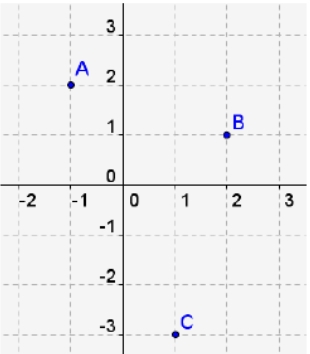
\includegraphics[width=2.58356in,height=2.95026in]{./_SAEB_9_MAT/media/image164.png}
\end{figure}

\begin{boxpeq}
\coment{$A = (-1, 2); B = (2, 1) e C = (1, -3)$.}
\end{boxpeq}

\num{2} O par ordenado de números que representa a igreja é:

\begin{figure}
\centering
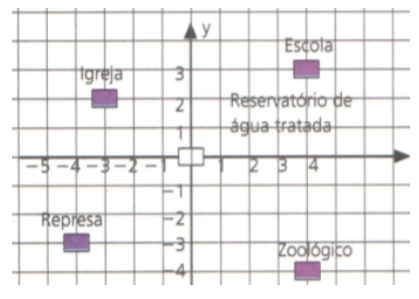
\includegraphics[width=2.7in,height=1.92673in]{./_SAEB_9_MAT/media/image165.png}
\end{figure}

\begin{boxpeq}
\coment{A igreja está localizada no ponto $(- 3, 2)$.}
\end{boxpeq}

\num{3} Uma formiga sai de um ponto x, anda 6 metros para a esquerda, 5
metros para cima, 2 metros para a direita, 2 metros para baixo, 6 metros
para a esquerda e 3 metros para baixo, chegando ao ponto y. Qual a
distância entre x e y?

\begin{boxpeq}
\coment{

\includegraphics[width=3.54197in,height=2.80024in]{./_SAEB_9_MAT/media/image166.png}
\end{boxpeq}

A distância percorrida pela formiga é de 10 metros.}

\num{4} Relacione as duas colunas ligando as planificações aos respectivos
objetos tridimensionais.

\begin{figure}
\centering
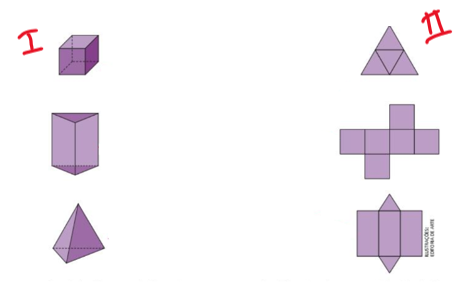
\includegraphics[width=3.45in,height=2.11404in]{./_SAEB_9_MAT/media/image167.png}
\end{figure}

\num{5} Um sólido geométrico convexo é formado por 8 faces triangulares, 10
faces quadrangulares e 12 faces hexagonais. Quantos vértices possui esse
sólido geométrico?

\begin{largebox}
\coment{Sabemos que o total de faces é igual a $8 + 10 + 12 = 30$. 
Para determinar o número de arestas, somamos todas e dividimos por 2, 
pois cada uma delas é compartilhada entre duas faces.

$ 8 \cdot 3 + 10 \cdot 4 + 12 \cdot 6 = 24 + 40 + 72 = 136 \rightarrow \\
136 \div 2 = 68$ arestas.
Pela relação de Euler $V + F = A + 2 \rightarrow V + 30 = 68 + 2 \rightarrow V = 40$.}
\end{largebox}

\num{6} Escreva os respectivos nomes dos segmentos
$\overline{\mathbf{\text{MN}}}$ e $\overline{\mathbf{\text{RS}}}$ e
das retas \textbf{a} e \textbf{b}:

\begin{figure}
\centering
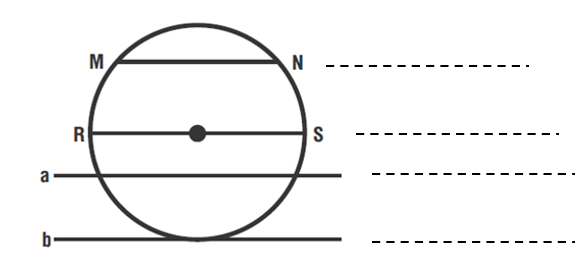
\includegraphics[width=4.87542in,height=2.25019in]{./_SAEB_9_MAT/media/image168.png}
\end{figure}

\reduline{$\overline{\mathbf{\text{MN}}}$ é corda.
$\overline{\mathbf{\text{RS}}}$ é o diâmetro.
A reta \textbf{a} é secante.
A reta \textbf{b} é tangente.\hfill}

\num{7} Considere as figuras planificadas I e II

\begin{figure}
\centering
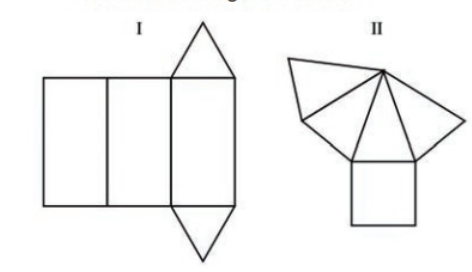
\includegraphics[width=3.93333in,height=2.18333in]{./_SAEB_9_MAT/media/image169.png}
\end{figure}

Estas planificações, ao serem montadas de maneira tridimensional,
gerarão respectivamente:

\begin{minipage}{.5\textwidht}
\begin{escolha}
  \item Prisma, Prisma

  \item Prisma, Cone

  \item Pirâmide, Prisma

  \item Prisma, Pirâmide
\end{escolha}
\end{minipage}
\sidetext{d) Correta. A figura I gerará um prisma triangular; a figura II, uma pirâmide
quadrangular.}

\num{8} Uma pirâmide com base hexagonal possui quantas faces e quantos
vértices?

\begin{boxpeq}
\coment{Uma pirâmide com base hexagonal terá seis faces triangulares (laterais),
mais a base hexagonal, contendo, portanto, 7 faces. Da mesma forma, terá os seis 
vértices da base e mais o do topo, em um total de 7 vértices.}
\end{boxpeq}

\num{9} Cuias indígenas são feitas por meio de técnicas e materiais tradicionais 
das culturas dos povos originários. Elas podem ser compostas de diferentes
materiais, como cabaça, madeira, bambu, taquara, entre outros, dependendo da
região e dos hábitos de cada povo.

As cuias são usadas para diversas finalidades, dependendo da
cultura em que são produzidas. Um exemplo de uso é armazenar e servir
alimentos e bebidas.

A parte superior de uma determinada cuia tem a forma de uma
circunferência de 60 cm de comprimento, como se observa na imagem a seguir.

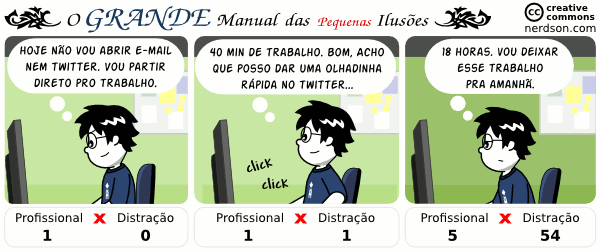
\includegraphics[width=2.31667in,height=1.40833in]{./_SAEB_9_MAT/media/image170.wmf}

Qual a medida em centímetros do raio dessa circunferência? Use \Pi = 3. 

\reduline{Como o comprimento da circunferência é dado por
$C = 2\Pi r = 2 \cdot 3 \cdot r = 60 \rightarrow r = 10$ cm.\hfill}

\num{10} Nomeie os ângulos ACD e ABD como um ângulo central ou ângulo
inscrito.

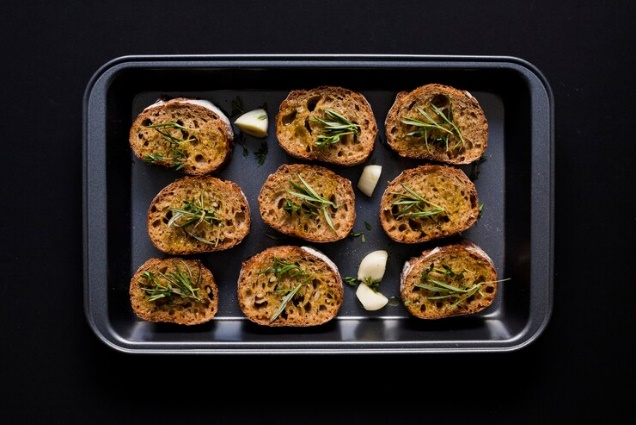
\includegraphics[width=2.425in,height=2.4in]{./_SAEB_9_MAT/media/image172.wmf}


\begin{itemize}
\item ACD é um ângulo \reduline{\textbf{central}, porque o vértice está no centro da
circunferência.\hfill}

\item ABD é um ângulo \reduline{\textbf{inscrito}, porque o vértice está sobre a circunferência.\hfill}
\end{itemize}

\section{Treino}

\num{1} Considere um poliedro convexo que possui oito vértices e apenas faces
triangulares e quadrangulares. Sabe-se que o número de faces
triangulares desse poliedro é quatro vezes maior do que o número de
faces quadrangulares. Determine a quantidade de arestas presentes nesse
poliedro.

Sabe-se que Vértice + Face = Aresta + 2

\begin{escolha}
  \item 20

  \item 16

  \item 10

  \item 8
\begin{escolha}


\num{2} Uma pirâmide que possui 6 vértices e 6 faces tem como base um:

\begin{escolha}
  \item triângulo

  \item quadrado

  \item pentágono

  \item hexágono
\end{escolha}


\num{3} Dos polígonos a seguir, indique aquele que é sempre regular.

\begin{escolha}
  \item Retângulo

  \item Triângulo isósceles

  \item Trapézio

  \item Quadrado
\end{escolha}

\chapter{Geometria II}
\markboth{Módulo 11}{}

\section{Habilidades do SAEB}

\begin{itemize}
  \item Identificar propriedades e relações existentes entre os elementos de um
triângulo (condição de existência, relações de ordem entre as medidas dos
lados e as medidas dos ângulos internos, soma dos ângulos internos,
determinação da medida de um ângulo interno ou externo).
  \item Classificar triângulos ou quadriláteros em relação aos lados ou aos
ângulos internos.
  \item Identificar retas ou segmentos de retas concorrentes, paralelos ou
perpendiculares.
  \item Identificar relações entre ângulos formados por retas paralelas cortadas
por uma transversal.
  \item Resolver problemas que envolvam relações entre ângulos formados por
retas paralelas cortadas por uma transversal, ângulos internos ou externos
de polígonos ou cevianas (altura, bissetriz, mediana, mediatriz) de
polígonos.
  \item Resolver problemas que envolvam relações métricas do triângulo
retângulo, incluindo o teorema de Pitágoras.
  \item Resolver problemas que envolvam polígonos semelhantes.
  \item Resolver problemas que envolvam aplicação das relações de
proporcionalidade abrangendo retas paralelas cortadas por transversais.
  \item Determinar o ponto médio de um segmento de reta ou a distância entre
dois pontos quaisquer, dadas as coordenadas desses pontos no plano
cartesiano.
\end{itemize} 

\section{Habilidades da BNCC}

\begin{itemize}
  \item EF09MA10, EF09MA13, EF09MA14, EF09MA16. 
\end{itemize}

\conteudo{
\begin{itemize}
        \item \textbf{Triângulos}
\end{itemize}

O triângulo pode ser classificado pela medida do lado ou pelos ângulos. 

Quando é classificado pelo \textbf{lado}, o triângulo pode ser:

    \begin{itemize}
    \item
      \textbf{Escaleno}: triângulo que possui todos os lados com medidas
  diferentes;
    \item
      \textbf{Isósceles}: triângulo que possui dois lados com medidas
  iguais;
    \item
      \textbf{Equilátero}: triângulo que possui todos os lados com medidas
  iguais.
    \end{itemize}

Quando é classificado pelo \textbf{ângulo}, o triângulo pode ser:

    \begin{itemize}
    \item
      \textbf{Acutângulo}: possui todos os ângulos internos menores que
  90°;
    \item
      \textbf{Obtusângulo}: possui exatamente um ângulo interno maior que
  90°;
    \item
      \textbf{Retângulo}: possui exatamente um ângulo interno igual a 90°.
    \end{itemize}

As principais \textbf{propriedades dos triângulos} são apresentadas a seguir.

    \begin{itemize}
    \item
  A soma dos ângulos internos de qualquer triângulo é sempre igual a
  180°;
    \item
  A soma dos ângulos externos de qualquer triângulo é sempre igual a
  360°;
    \item
  A soma das medidas de dois lados de um triângulo é sempre maior que a
  medida do terceiro lado. Essa propriedade é chamada de    \textbf{desigualdade
  triangular}. Trata-se da condição de existência do triângulo.
    \end{itemize}

\begin{itemize}
        \item \textbf{Paralelas cortadas por uma transversal}
\end{itemize}

Duas retas distintas são paralelas quando possuem a mesma inclinação, ou
seja, possuem o mesmo coeficiente angular. Além disso, a distância entre
elas é sempre a mesma e não possuem pontos em comum (não se cruzam).

Sejam duas retas \textbf{r} e \textbf{s}, paralelas entre si e uma transversal 
\textbf{t}, não perpendicular a \textbf{r} e \textbf{s}. Temos que os 8 (oito)
ângulos formados pela reta transversal com as retas \textbf{r} e \textbf{s}, 
quatro deles serão agudos (\alpha) e congruentes (mesma medida), os outros quatro
serão obtusos (\beta) e congruentes. Além disso, os ângulos obtusos e agudos serão 
suplementares (medem 180°).


\includegraphics[width=1.96354in,height=1.3968in]{./_SAEB_9_MAT/media/image186.png}
}

\section{Atividades}

\num{1} Determine o valor de x e os valores dos ângulos A e B.

\begin{figure}
\centering
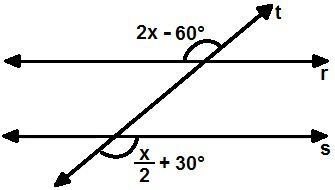
\includegraphics[width=2.83333in,height=1.60939in]{./_SAEB_9_MAT/media/image187.jpeg}
\end{figure}

%Autor: Montar figura semelhante, colocando o ângulo 2x -- 60º = A e o ângulo x/2 + 30º = B

\begin{boxmedio}
\coment{Pela figura, sabemos que os ângulos alternos externos são congruentes, ou
seja, A = B.

$2x - 60 = \frac{x}{2} + 30$ \\
$2x - \frac{x}{2} = 30 + 60 \rightarrow \\
\frac{4x - x}{2} = 90 \rightarrow \\
\frac{3}{2}x = 90 \rightarrow x = 60$

X = 60°, A = B = 60°.}
\end{boxmedio}

\num{2} Um retângulo foi desenhado em um plano cartesiano, com altura
determinada pelos vértices dos pontos A e B de coordenadas (1, 3) e (1,
4), respectivamente. Além disso, sabe-se que um ponto M de
coordenadas (3, 3) é o ponto médio da base do retângulo.

Qual é a área desse retângulo?

\begin{boxpeq}
\coment{Construindo o retângulo com vértices em A e B, podemos perceber que sua
altura será igual a 1 unidade. A distância entre o ponto A (1,3) e M
(3,3) é de 2 unidades. Dado que M é ponto médio da base, podemos afirmar
que a base tem 4 unidades. Assim, para determinar a área, basta fazer 
$1 \cdot 4 = 4$ unidades quadradas de área.}
\end{boxpeq}

\num{3} Leio o texto a seguir.

\begin{quote}
\textbf{Futebol e Matemática}

° bola de futebol utilizada na Copa de 2010, na África do Sul, ganhou o
apelido de ``Jabulani'' e foi criticada pelos jogadores por ser mais
simples do que as bolas utilizadas desde a década de 1970, que
apresentam uma estrutura icosaedro truncado com 32 faces compostas por
12 pentágonos regulares e 20 hexágonos regulares. Cada um dos 60
vértices do icosaedro tr° é formado pela união de um pentágono e
dois hexágonos, resultando em 90 arestas para o sólido.
\end{quote}

Qual soma dos ângulos internos do pentágono e hexágono respectivamente?

\begin{boxmedio}
\coment{A soma dos ângulos internos é dada por:

$S = (n - 2)\cdot 180$° 

Para pentágono temos: $S = 3 \cdot 180 = 540$°

Para hexágono temos: $S = 4 \cdot 180 = 720$°}
\end{boxmedio}

\num{4} Um estudante fez um polígono inscrito em um círculo. Para executar
essa tarefa, ele dividiu o círculo em cinco arcos de mesma medida, e
marcou os pontos A, B, C, D e E.

\begin{figure}
\centering
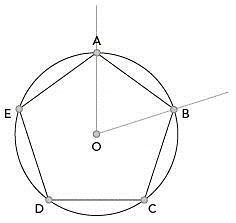
\includegraphics[width=2.45291in,height=2.3178in]{./_SAEB_9_MAT/media/image188.png}
\end{figure}

Determine a medida de AOB.

\begin{boxpeq}
\coment{Como a circunferência foi dividida em 5 arcos, basta fazer $360 \div 5 =
72$°. Como AOB é ângulo central, a medida do ângulo e arco é a mesma.}
\end{boxpeq}

\num{5} Um polígono com ângulos centrais medindo 40° tem quantos lados? Qual
a medida do ângulo interno deste mesmo polígono?

\begin{boxpeq}
\coment{Como o ângulo central tem medida 40°, podemos determinar o número de
lados do polígono utilizando o Ângulo de 360°: $360 \div 40 = 9$. O polígono
tem 9 lados. A soma dos ângulo internos é dada por $S = 7 \cdot 180 = 1260$,
logo cada ângulo interno é dado por $1260 \div 9 = 140$°.}
\end{boxpeq}

\num{6} Entre as medidas dos palitos dadas abaixo, quais delas impossibilitam a
formação de um triângulo?

\begin{enumerate}
  \item Três palitos de 7 cm cada;
 
  \item Dois palitos de 7 cm e um palito de 15 cm;

  \item Dois palitos de 10 cm e um palito de 13 cm;
 
  \item Um palito de 10 cm, um de 13 cm e outro de 15 cm.
\end{enumerate}

\begin{boxmedio}
\coment{Para testar a condição de existência de um triângulo, é preciso
verificar se a soma das medidas de dois lados quaisquer é maior do que a
medida do terceiro lado. Em II, a soma das medidas de dois lados quaisquer 
é igual a 14 cm, que é menor do que a medida do terceiro lado, que é de 15 cm.
Não é possível, portanto, construir um triângulo com dois palitos de 7 cm e 
um palito de 15 cm.}
\end{boxmedio}

\num{7} João montou um triângulo retângulo utilizando régua e compasso. Os
catetos formados tinham as medidas 12 cm e 16 cm. Com isso qual será a
medida do terceiro lado?

\begin{boxmedio}
\coment{Pelo teorema de Pitágoras temos:

$x^2 = 12^2 + 16^2 \\
x^2 = 144 + 256 \\
x^2 = 400 \rightarrow x = 20$.

Também é possível utilizar o triângulo 3, 4 e 5 e perceber que ele é
semelhante ao triângulo do problema com razão de proporção 4. Ou seja,
bastaria fazer $4 \cdot 5 = 20$.}
\end{boxmedio}

\num{8} Ao tentar construir um triângulo escaleno, ou seja, como todos os
lados diferentes, quais são as opções para o terceiro lado, com medida
inteira, sabendo que os dois primeiros lados têm a medida 3 e 4?

\begin{boxmedio}
\coment{Para construir um triângulo escaleno, é preciso que os três lados tenham
medidas diferentes. Se dois lados desse triângulo tiverem medidas
respectivamente iguais a 3 e 4, o terceiro lado só poderá ter uma medida
que não seja 3 nem 4.

Descartamos o valor 1, pois a soma com 3 daria 4 que é a medida de um dos
lados. Pelo critério de existência do triângulo podemos usar os valores:
2, 5 e 6.}
\end{boxmedio}

\num{9} Na figura a seguir, verifica-se que os terrenos demarcados estão 
localizados entre a Ruas das Rosas e a Rua das Flores. O proprietário pode 
optar por construir a frente da casa para qualquer uma dessas ruas. Qual a 
medida, em metros, dos lotes na Rua das Flores?

\begin{figure}
\centering
\includegraphics[width=2.89167in,height=1.99596in]{./_SAEB_9_MAT/media/image189.png}
\end{figure}

\begin{boxmedio}
\coment{Os cálculos podem ser efetuados por meio do Teorema de Tales. Fazendo a
proporção para determinar os valores:

$\frac{20}{x} = \frac{50}{64} \rightarrow 50x = 1.280 \rightarrow x = 25,6$
$\frac{60}{x} = \frac{50}{64} \rightarrow 50x = 3.840 \rightarrow x = 76,8$}
\end{boxmedio}

\num{10} Determine o valor de \alpha, sabendo que temos uma figura formada por 2
quadrados e um triângulo equilátero.

\begin{figure}
\centering
\includegraphics[width=2.90025in,height=1.35012in]{./_SAEB_9_MAT/media/image190.png}
\end{figure}

\begin{boxpeq}
\coment{Dado a formação com dois quadrados e um triângulo equilátero, temos:

\begin{figure}
\includegraphics[width=2.975in,height=1.53351in]{./_SAEB_9_MAT/media/image191.png}
\end{figure}

Temos que $x = 60$° e $y = 90$°. Dessa forma, \alpha será igual a:

$\alpha + 90 + 90 + 60 = 360$, pois fecha a circunferência. Logo podemos
afirmar que $\alpha = 120$°.}
\end{boxpeq}

\section{Treino}

\num{1} Um portão é formado por barras de fecho:

\includegraphics[width=3.36667in,height=1.51667in]{./_SAEB_9_MAT/media/image192.png}{]}

Determine a medida da barra que está na diagonal.

\begin{escolha}
  \item 2

  \item 2,5
  
  \item 3
  
  \item 4
\end{escolha}


\num{2} Qual figura representa um trapézio escaleno?

\begin{figure}
\centering
\includegraphics[width=3.44197in,height=1.9335in]{./_SAEB_9_MAT/media/image193.png}
\end{figure}

\begin{escolha}

  \item I

  \item II

  \item III

  \item IV
\end{escolha}


\num{3} Observe a imagem a seguir, que apresenta paralelas cortadas por retas
transversais.

\begin{figure}
\centering
\includegraphics[width=3.65833in,height=1.84637in]{./_SAEB_9_MAT/media/image194.jpeg}
\end{figure}

Determine o valor de x.

\begin{escolha}
  \item 12°

  \item 20°

  \item 24°

  \item 48°
\end{escolha}


\chapter{Deslocamento usando coordenadas}
\markboth{Módulo 12}{}

\section{Habilidades do SAEB}

\begin{itemize}
  \item Descrever ou esboçar deslocamento de pessoas e/ou de objetos em
representações bidimensionais (mapas, croquis etc.), plantas de
ambientes ou vistas, de acordo com condições dadas.   

\end{itemize} 

\conteudo{
%Obs Rogério, 16/5/23, 10h35: o texto abaixo é bastante semelhante ao que está disponível em https://portal.educacao.go.gov.br/wp-content/uploads/2021/02/Atividade-2-Tema-Localizacao-e-movimentacao-representacao-de-objetos-e-pontos-de-referencia-3o-ano.pdf

\textbf{Localização e movimentação}

Interpretar e construir representações espaciais são habilidades
fundamentais para a vida cotidiana das pessoas em diversas situações.
Compreender noções como trajetória, direção e sentido é essencial para
se localizar e comunicar posições e deslocamentos, tanto em ambientes
menores, como a sala de aula ou a própria casa, quanto em ambientes
maiores, como a cidade.

Ao interpretar uma representação espacial, é preciso selecionar
referências para se localizar e entender as informações presentes. Essas
referências podem ser pontos de referência físicos, como um edifício
alto ou uma praça, ou pontos de referência abstratos, como um cruzamento
ou uma interseção de ruas.

Ao construir uma representação espacial, é necessário ter em mente as
noções de trajetória, direção e sentido para indicar com precisão a
posição e o deslocamento de objetos ou pessoas. Além disso, é importante
utilizar símbolos e legendas adequados para tornar a representação clara
e compreensível.

Em resumo, interpretar e construir representações espaciais, localizar
objetos e comunicar posições e deslocamentos são habilidades
fundamentais para a vida cotidiana. O entendimento de noções como
trajetória, direção e sentido é essencial para se localizar e
interpretar informações em ambientes de dimensões menores e maiores.

\textbf{Trajetória}

A trajetória é o caminho percorrido por um objeto, pessoa ou evento em
uma sequência de pontos, desde o ponto de partida até o ponto de
chegada. Ao longo da trajetória, podem existir pontos fixos que servem
como referência para a localização e orientação.

A trajetória pode apresentar deslocamentos em linha reta ou em linha
curva, dependendo do percurso que é seguido. A direção indica a
orientação em que o deslocamento ocorre, enquanto o sentido indica a
orientação em relação ao ponto de partida.

É importante entender e interpretar a trajetória, a direção e o sentido
em diversas situações do cotidiano, como na locomoção em uma cidade ou
na navegação em um mapa. Compreender essas noções é fundamental para se
orientar e se deslocar com segurança e eficiência.

Por exemplo, o deslocamento da Praça da Sé na cidade de São Paulo até a
NeoQuímica Arena (Arena Corinthians).

\includegraphics[width=3.39062in,height=1.68534in]{./_SAEB_9_MAT/media/image196.png}

\fonte{Google Maps. Disponível em: https://goo.gl/maps/cfVtjYA7ydh7rzjb7. 
Acesso em 16 mai. 2023}

}

\section{Atividades}

\num{1} Gustavo e Heitor utilizaram um tabuleiro quadriculado como tabuleiro
de um ``jogo da velha'', no qual as linhas são identificadas por letras,
e as colunas por números. Durante uma partida, Gustavo decidiu começar
o jogo pela casa destacada em cinza.

\includegraphics[width=1.5918in,height=1.55847in]{./_SAEB_9_MAT/media/image197.png}

%Autor: Construir a figura semelhante

Qual é a coordenada com que o Gustavo decidiu começar a jogada?

\reduline{Gustavo começou pela casa G3.\hfill}

\num{2} Observando um tabuleiro de xadrez com algumas peças, escreva a posição
da peça no tabuleiro.

\includegraphics[width=0.27083in,height=0.27639in]{./_SAEB_9_MAT/media/image198.png}

\begin{figure}
\centering
\includegraphics[width=2.40278in,height=2.27161in]{./_SAEB_9_MAT/media/image199.png}
\end{figure}


\reduline{A peça está na casa I3.\hfill}

\num{3} Observe o mapa a seguir.

\begin{figure}
\centering
\includegraphics[width=2.74306in,height=2.00374in]{./_SAEB_9_MAT/media/image200.png}
\end{figure}


Eloísa disse para sua amiga Lara que mora numa rua entre as avenidas A e
B e entre as ruas da igreja e da locadora. Sendo assim, em qual rua Eloísa
mora?

\reduline{Entre as avenidas A e B temos as ruas 2 e 4, mas entre a Igreja e
locadora temos a rua 4. Essa é a rua da casa da Eloísa.\hfill}

\num{4} Considerando o mapa da região onde Lucas mora, escreva a localização
da escola.

\begin{figure}
\centering
\includegraphics[width=1.71528in,height=1.71528in]{./_SAEB_9_MAT/media/image201.png}
\caption{Diagrama Descrição gerada automaticamente}
\end{figure}

%Autor: Montar uma imagem semelhante 
%Autor: Deixe 1 linhas (pode ser na lateral da imagem)

\linhas{1}
\coment{A escola está na coluna 3, linha E.}

\num{5} O mapa abaixo é de um bairro, em que cada quadrado representa um
quarteirão. A medida do lado de cada quadrado é de 100m.

\begin{figure}
\centering
\includegraphics[width=2.4375in,height=1.82292in]{./_SAEB_9_MAT/media/image202.png}
\caption{Imagem em branco e preto Descrição gerada automaticamente com
confiança média}
\end{figure}

%Autor: Fazer imagem semelhante, os dados são importantes

Maria saiu da esquina indicada pelo ponto Q e cumpriu o seguinte
percurso:

\begin{itemize}
  \item caminhou 500 metros na direção Norte;

  \item depois caminhou 200 metros na direção Oeste;
  
  \item a seguir caminhou 300 metros na direção Sul;
  
  \item finalmente, caminhou mais 200 metros na direção Oeste.
\end{itemize}

Ao final desse percurso, Maria alcançou a esquina indicada por qual letra?

\coment{\begin{figure}
\centering
\includegraphics[width=1.50277in,height=1.45139in]{./_SAEB_9_MAT/media/image203.png}
\caption{Tela de celular Descrição gerada automaticamente com confiança
baixa}
\end{figure}
%Autor: Fazer imagem semelhante, os dados são importantes

Ao final do percurso, Maria alcançou a esquina indicada pela letra S.} 

\num{6} Luís Felipe criou uma planta da sua casa para um trabalho da escola.

\begin{figure}
\centering
\includegraphics[width=2.52083in,height=1.18147in]{./_SAEB_9_MAT/media/image204.png}
\caption{Diagrama Descrição gerada automaticamente}
\end{figure}

%Autor: Fazer imagem semelhante, os dados são importantes 

Ao entrar pela porta da sala, virar à esquerda, seguir até o final do
corredor e virar a esquerda novamente, em qual cômodo Luís Felipe entrou?

\linhas{1}

\coment{
\begin{figure}
\centering
\includegraphics[width=3.28362in,height=1.58347in]{./_SAEB_9_MAT/media/image205.png}
\caption{Diagrama Descrição gerada automaticamente}
\end{figure}

% Fazer imagem semelhante, é importante os dados
Depois de fazer o percurso indicado, Luiz Felipe chegou ao Quarto 1.}

\num{7} João, de bicicleta, e Marcos, a pé, resolveram disputar uma corrida diferente, 
entre os pontos A e B, partindo simultaneamente de A e deslocando-se
rigorosamente sobre as linhas tracejadas das alamedas.

\begin{figure}
\centering
\includegraphics[width=3.00694in,height=1.36847in]{./_SAEB_9_MAT/media/image206.png}
\caption{Diagrama Descrição gerada automaticamente}
\end{figure}

%Fazer imagem semelhante, é importante os dados
Qual a diferença, em metros, da distância percorrida por cada um deles?

\linhas{2}
\coment{João percorreu $150 + 150 + 250 + 250 + 150 + 150 = 1.100$ metros. 
Marcos, por sua vez, percorreu $250 + 250 = 500$ m.
A diferença entre as distâncias percorridas por eles é $1.100 - 500 = 600$ metros.}

\num{8} O mapa de uma região de uma cidade do interior está representado na
figura abaixo.

\begin{figure}
\centering
\includegraphics[width=2.96528in,height=2.96528in]{./_SAEB_9_MAT/media/image207.png}
\caption{Diagrama Descrição gerada automaticamente}
\end{figure}

%Autor: Fazer imagem semelhante, é importante os dados

Jorge saiu da praça central e, orientando-se por esse mapa, caminhou 3
quadras na direção oeste e, depois, 2 quadras na direção sul. Em qual
local Jorge chegou?

\linhas{1}
\coment{Percorrendo o caminho indicado, Jorge chegou ao Posto de Saúde, como 
se verifica na figura a seguir.

\begin{figure}
\centering
\includegraphics[width=1.95139in,height=1.84648in]{./_SAEB_9_MAT/media/image208.png}
\caption{Diagrama Descrição gerada automaticamente}
\end{figure}
}

\num{9} Carlos precisa sair do ponto A e chegar ao ponto D. Faça a indicação
do menor caminho para interligar esses pontos.

\begin{figure}
\centering
\includegraphics[width=2.40278in,height=1.53858in]{./_SAEB_9_MAT/media/image209.jpeg}
\caption{Calendário Descrição gerada automaticamente}
\end{figure}

%Fazer imagem semelhante, é importante os dados

\linhas{2}
\coment{Carlos deve sair do ponto A pela Avenida da Orla por 1 quarteirão,
virar à direita na Rua Paraguai e seguir até o cruzamento dessa rua com a Avenida
Projetada.}

\num{10} Um turista caminhou por todos os pontos turísticos indicados no mapa a seguir.
As distâncias entre os pontos estão em quilômetros.

\begin{figure}
\centering
\includegraphics[width=2.77778in,height=2.5in]{./_SAEB_9_MAT/media/image210.png}
\caption{Mapa Descrição gerada automaticamente}
\end{figure}

%Fazer imagem semelhante, é importante os dados

Considerando que o turista saiu de A, passou por B, C, D, E e retornou ao ponto A,
responda: qual a distância total percorrida, em km?

\linhas{1}
\coment{$90 + 153 + 121 + 239 + 117 = 720$ km.}

\section{Treino}

\num{1} Observe a imagem a seguir.

%Fazer imagem semelhante, é importante os dados

%ATENÇÃO: faltou a imagem aqui. Tem no original.

Qual a distância entre a casa da Sílvia e a de Paula?

\begin{escolha}

  \item 100 m

  \item 200 m

  \item 300 m

  \item 400 m

\end{escolha}

\coment{SAEB: Descrever ou Esboçar o deslocamento de pessoas e/ou objetos em representações bidimensionais (mapas, croquis etc.), plantas de ambientes ou vistas, de acordo com condições dadas.

a) Incorreta. A distância entre a casa de Sílvia e a de Paula é de 400 m.
b) Incorreta. A distância entre a casa de Sílvia e a de Paula é de 400 m.
c) Incorreta. A distância entre a casa de Sílvia e a de Paula é de 400 m.
d) Correta. A distância entre a casa de Sílvia e a de Paula é de 400 m:  2 quadras 
ao Sul (200m) e duas quadras ao Leste (200m).}

\num{2} Qual é a melhor maneira de determinar sua localização exata em um
mapa? 

\begin{escolha}

  \item Usando um sistema de orientação, como uma bússola ou GPS. 

  \item Estimando sua posição com base em pontos de referência próximos. 

  \item Adivinhando sua posição com base em sua experiência anterior na área. 

  \item Olhando para o mapa e tentando comparar com o ambiente ao seu redor.

\end{escolha}

\coment{SAEB: Descrever ou Esboçar o deslocamento de pessoas e/ou objetos em representações bidimensionais (mapas, croquis etc.), plantas de ambientes ou vistas, de acordo com condições dadas.

a) Correta. Sistemas de orientação, como uma bússola ou GPS, são bem mais precisos do que
as formas de determinação de localização descritas nas outras alternativas.
b) Incorreta. Sistemas de orientação, como uma bússola ou GPS, são bem mais precisos do que 
estimativas de posição com base em pontos de referência.
c) Incorreta. Sistemas de orientação, como uma bússola ou GPS, são bem mais precisos do que 
adivinhações com base em experiência pessoal.
d) Incorreta. Sistemas de orientação, como uma bússola ou GPS, são bem mais precisos do que
visualização de mapas.} 

\num{3} Determine a distância entre a casa de Lucas e a escola.

\begin{figure}
\centering
\includegraphics[width=3.29167in,height=1.79167in]{./_SAEB_9_MAT/media/image212.png}
\caption{Diagrama Descrição gerada automaticamente}
\end{figure}

%Autor: Fazer imagem semelhante, é importante os dados

\begin{escolha}

  \item 3 Norte e 2 Leste

  \item 2 Norte e 3 Leste

  \item 5 Sul e 2 Oeste

  \item 3 Norte e 4 Leste

\end{escolha}

\coment{SAEB: Descrever ou Esboçar o deslocamento de pessoas e/ou objetos em representações bidimensionais (mapas, croquis etc.), plantas de ambientes ou vistas, de acordo com condições dadas.

a) Correta. A distância entre a casa de Lucas e a escola é de 3 quadras a Norte e 2 a 
Leste.
b) Incorreta. A distância entre a casa de Lucas e a escola é de 3 quadras a Norte e 2 a 
Leste.
c) Incorreta. A distância entre a casa de Lucas e a escola é de 3 quadras a Norte e 2 a 
Leste.
d) Incorreta. A distância entre a casa de Lucas e a escola é de 3 quadras a Norte e 2 a 
Leste.}

\chapter{Estatística}
\markboth{Módulo 13}{}

\section{Habilidades do SAEB}

\begin{itemize}

  \item Identificar os indivíduos (universo ou população alvo da pesquisa), as
variáveis e os tipos de variáveis (quantitativas ou categóricas) em um
conjunto de dados.
  \item Representar ou associar os dados de uma pesquisa estatística ou de um
levantamento em listas, tabelas (simples ou de dupla entrada) ou gráficos
(barras simples ou agrupadas, colunas simples ou agrupadas, pictóricos,
de linhas, de setores, ou em histograma).
  \item Inferir a finalidade da realização de uma pesquisa estatística ou de um
levantamento, dada uma tabela (simples ou de dupla entrada) ou gráfico
(barras simples ou agrupadas, colunas simples ou agrupadas, pictóricos,
de linhas, de setores ou em histograma) com os dados dessa pesquisa. 
  \item Interpretar o significado das medidas de tendência central (média
aritmética simples, moda e mediana) ou da amplitude. 
  \item Calcular os valores de medidas de tendência central de uma pesquisa
estatística (média aritmética simples, moda ou mediana). 
  \item Resolver problemas que envolvam dados estatísticos apresentados em
tabelas (simples ou de dupla entrada) ou gráficos (barras simples ou
agrupadas, colunas simples ou agrupadas, pictóricos, de linhas, de setores
ou em histograma). 
  \item Argumentar ou analisar argumentações/conclusões com base nos dados
apresentados em tabelas (simples ou de dupla entrada) ou gráficos (barras
simples ou agrupadas, colunas simples ou agrupadas, pictóricos, de linhas,
de setores ou em histograma). 
  \item Explicar/descrever os passos para a realização de uma pesquisa
estatística ou de um levantamento.

\end{itemize} 

\section{Habilidades da BNCC}

\begin{itemize}
  \item EF09MA21, EF09MA22.
\end{itemize}

\conteudo{A \textbf{moda}, a \textbf{média} e a \textbf{mediana} são medidas de
tendência central usadas na estatística para resumir um conjunto de dados.

A \textbf{moda} é o valor mais comum em um conjunto de dados, ou seja, é o valor
que aparece com mais frequência. É útil para dados discretos e pode ser
usada em combinação com outras medidas de tendência central.

A \textbf{média} é a soma de todos os valores em um conjunto de dados dividida
pelo número de valores. É a medida mais comum de tendência central e é
útil para dados contínuos. No entanto, é sensível a valores extremos,
que podem distorcer o resultado.

A \textbf{mediana} é o ``valor do meio'' em um conjunto de dados quando eles são
colocados em ordem crescente ou decrescente. É uma medida robusta de
tendência central, ou seja, é menos afetada por valores extremos do que
a média. A mediana é útil para dados com valores extremos ou
distribuição assimétrica. Para calcular a mediana organizam-se os dados
de forma crescente ou decrescente. Esta lista é o \textbf{rol} de dados. 
Depois de organizar os dados, verificamos se a quantidade de dados no rol
é par ou ímpar.

\begin{itemize}
\item
  Se a quantidade de dados no rol é ímpar, a mediana é o valor do meio,
  da posição central;
\item
  Se a quantidade de dados no rol é par, a mediana é a média aritmética
  dos valores centrais;
\end{itemize}

Em geral, a escolha da medida de tendência central depende da natureza
dos dados e do objetivo da análise estatística. Cada medida pode ser
útil em diferentes contextos e situações.
}

\section{Atividades}

\num{1} Complete as lacunas a seguir.

No 1° trimestre, João tirou as notas parciais 5,0 na Prova 1 e 3,0 na
Prova 2. Portanto sua média foi \_\_\_. No entanto, se tivesse tirado
\_\_\_ na segunda prova, sua média seria 6,0.

%BNCC: EF09MA21 SAEB: 9E1.4

\coment{A média é $\frac{5 + 3}{2} = 4$. Com a segunda prova igual a 6,0, a
média seria $\frac{5 + 6}{2} = 5,5$.}

\num{2} Carlos e Anderson tiveram a mesma média final na disciplina de Álgebra.
Carlos tirou 7,0 e 5,0. Anderson tirou 8,0 em uma das provas. Qual foi a nota 
de Anderson na segunda prova?

\linhas{2}

%BNCC: EF09MA21 SAEB: 9E1.4

\coment{A média de Carlos é: $\frac{7 + 5}{2} = 6$. Em uma das provas, Anderson 
tirou 8,0. A média de Anderson também é 6, de modo que
$\frac{x + 8}{2} = 6 \rightarrow x + 8 = 12 \rightarrow x = 4$.}

\num{3} Construa um gráfico de setor com base na tabela a seguir,
representando-a em porcentagem.

% Please add the following required packages to your document preamble:
% \usepackage[table,xcdraw]{xcolor}
% If you use beamer only pass "xcolor=table" option, i.e. \documentclass[xcolor=table]{beamer}
\begin{table}[]
\begin{tabular}{|c|c|}
\hline
\rowcolor[HTML]{DAE8FC} 
\textbf{Marca} & \textbf{Pessoas} \\ \hline
A & 30 \\ \hline
B & 70 \\ \hline
C & 45 \\ \hline
D & 55 \\ \hline
\end{tabular}
\end{table}

\begin{largebox}

%BNCC: EF09MA22 SAEB: 9E1.4

\coment{
\begin{figure}
\centering
\includegraphics[width=2.41667in,height=2.43637in]{./_SAEB_9_MAT/media/image213.png}
\caption{Gráfico, Gráfico de pizza Descrição gerada automaticamente}
\end{figure}
}

\num{4} Uma loja fez um levantamento para saber como estava distribuído o
atendimento dos clientes ao longo do dia. O objetivo dessa pesquisa era decidir
sobre novas contratações para atender o horário com maior fluxo de clientes.

\begin{figure}
\centering
\includegraphics[width=3.32598in,height=2.58268in]{./_SAEB_9_MAT/media/image214.jpg}
\caption{1632731228879\_1622599524064\_3568a1d3-2f50-427b-8eea-c95bc06e8bfe.jpg}
\end{figure}

%Montar figura semelhante

Qual horário deve ter mais funcionários para atender?

%BNCC: EF09MA22 SAEB: 9E1.4

\coment{Dada a distribuição dos horários, é perceptível que a grande maioria dos
clientes frequenta a loja das 8h às 12h.}

\num{5} Foi realizada uma pesquisa sobre a possibilidade de antecipar o horário
de início das aulas de uma grande escola: em vez de começar às 7h30, elas se iniciariam
às 7h. 3700 famílias responderam à pesquisa e tiveram suas respostas tabuladas e
colocadas em um gráfico de setores.

\begin{figure}
\centering
\includegraphics[width=3.34677in,height=1.96063in]{./_SAEB_9_MAT/media/image215.jpg}
\caption{1632731350522\_1622599544538\_67a4b9ce-09b6-4c36-83bb-b178065a1133.jpg}
\end{figure}

%Fazer uma nova imagem

Com base nas informações do gráfico, quantas pessoas concordaram com a mudança?

%BNCC: EF09MA22 SAEB: 9E2.1

\coment{Para obter o número de pessoas que concordaram com a mudança, é preciso
calcular 22\% de 3700 = $0,22 \cdot 3700 = 814$ pessoas.}

\num{6} Em uma aula de Matemática os estudantes receberam a tarefa de medir a
largura da sala. Após a medição, os estudantes colocaram os resultados
encontrados na lousa. 5,35; 5,21; 5,74; 5,19; 4,96; 5,80; 5,56; 5,94; 5,56; 
4,98; 6,10; 5,38; 5,74; 5,65. Ao perceber que os alunos não foram precisos nas
medidas, o professor perguntou quais são os valores de moda e mediana dessas medidas.

Responda à pergunta do professor.

\begin{boxmedio}

\coment{Primeiramente, é necessário organizar o rol de informações: 4,96; 4,98; 5,19; 5,21; 5,35; 5,38; 5,56; 5,56; 5,58; 5,74; 5,74; 5,74; 5,94; 6,1.

A seguir, percebe-se que a \textbf{moda} é 5,74, porque essa é a medida que se
repete mais vezes. Como temos 14 elementos, uma quantidade par, a mediana é obtida
pela média aritmética entre o 7º e 8º elementos do rol. Como ambos tem o mesmo valor, 
5,56, a \textbf{mediana} é 5,56.}

\num{7} Uma cidade investiu em tratamento de água de chuva. A análise da água
tratada revelou os dados apresentados no gráfico da quantidade em $m^3$ por
mês.

\begin{figure}
\centering
\includegraphics[width=4.95586in,height=2.50694in]{./_SAEB_9_MAT/media/image216.jpg}
\caption{1632731306179\_1622601258507\_1318b98e-1363-40cc-af30-a8e7cb6c0ecc.jpg}
\end{figure}

%Fazer novo gráfico

\begin{escolha}

  \item Qual mês registrou a menor quantidade e qual registrou a maior
  quantidade de água de chuva tratada nesse período?

\linhas{1}

\coment{A menor quantidade foi registrada no mês de maio com $2m^3$ e a maior foi
  em outubro com $11m^3$.}

  \item Sabendo que em junho foram tratados $6m^3$ de água, qual a porcentagem
  de aumento para o mês de setembro?

\linhas{2}

\coment{Como em junho foram tratados $6m^3$ de água e em setembro foram tratados
  $10m^3$, houve um aumento de $4m^3$ -- o que representa um aumento
  aproximado de 66,67\%}

\end{escolha}

\num{8} O gráfico a seguir representa a quantidade de casas que uma
imobiliária alugou em cada mês em uma determinada cidade.

\begin{figure}
\centering
\includegraphics[width=3.21165in,height=1.77953in]{./_SAEB_9_MAT/media/image217.jpg}
\caption{1632730655835\_1622599672828\_f1b500eb-5b86-4a39-b7df-d128c164df02.jpg}
\end{figure}

%Montar gráfico semelhante.

Qual é a mediana da quantidade de casas alugadas?

\coment{Primeiramente, é necessário organizar o rol de informações: 
10; 15; 15; 20; 30; 35. Por ter 6 elementos, a mediana é
determinada pela média aritmética entre os elementos centrais que são 15
e 20, ou seja, a mediana é dada pelo valor 17,5.}

\num{9} Uma auditoria de uma montadora do grande ABC paulista levantou os dados 
da tabela a seguir.

% Please add the following required packages to your document preamble:
% \usepackage[table,xcdraw]{xcolor}
% If you use beamer only pass "xcolor=table" option, i.e. \documentclass[xcolor=table]{beamer}
\begin{table}[]
\begin{tabular}{c|c|c}
\hline
\rowcolor[HTML]{C0C0C0} 
\multicolumn{1}{|c|}{\cellcolor[HTML]{C0C0C0}\textbf{Montadora}} & \textbf{Unidades produzidas} & \multicolumn{1}{c|}{\cellcolor[HTML]{C0C0C0}\textbf{\% da produção da venda}} \\ \hline
A & 1000 & 60\% \\ \hline
B & 1500 & 80\% \\ \hline
C & 2000 & 50\% \\ \hline
\end{tabular}
\end{table}

%Montar tabela

Componha o gráfico que melhor representa a quantidade da produção vendida por
essas três montadoras.

%Mensagem do Rogério, em 17/3: o que aconteceu aqui é transformei uma questão de múltipla escolha em questão aberta. Só fiquei preocupado se a supressão das imagens abaixo não prejudica a montagem do arquivo, por isso mantive tudo como comentário. A imagem utilizada no gabarito da questão aberta é a alternativa C da questão original. 
%Montar os gráficos de cada alternativa, importante os títulos dos eixos
%a)
%\begin{figure}
%\centering
%\includegraphics[width=1.85016in,height=1.57514in]{./_SAEB_9_MAT/media/image219.png}
%\caption{Gráfico, Gráfico de barras Descrição gerada automaticamente}
%\end{figure}
%b)
%\begin{figure}
%\centering
%\includegraphics[width=1.84183in,height=1.43346in]{./_SAEB_9_MAT/media/image220.png}
%\caption{Gráfico, Gráfico de barras Descrição gerada automaticamente}
%\end{figure}
%c)
%\begin{figure}
%\centering
%\includegraphics[width=2.01684in,height=1.90017in]{./_SAEB_9_MAT/media/image221.png}
%\caption{Gráfico, Gráfico de barras Descrição gerada automaticamente}
%\end{figure}
%d)
%\begin{figure}
%\centering
%\includegraphics[width=1.89183in,height=2.26686in]{./_SAEB_9_MAT/media/image222.png}
%\caption{Gráfico, Gráfico de barras Descrição gerada automaticamente}
%\end{figure}
%BNCC: EF09MA21 SAEB: 9E1.2

\coment{
\begin{figure}
\centering
\includegraphics[width=2.01684in,height=1.90017in]{./_SAEB_9_MAT/media/image221.png}
\caption{Gráfico, Gráfico de barras Descrição gerada automaticamente}
\end{figure}
}

\num{10} Uma loja de queijos fez a contagem de queijos canastra vendidos ao
longo de 2022 em forma de pictograma, como se pode verificar na imagem abaixo. 

\begin{figure}
\centering
\includegraphics[width=2.97917in,height=1.71639in]{./_SAEB_9_MAT/media/image223.png}
\caption{Uma imagem contendo Texto Descrição gerada automaticamente}
\end{figure}

% Autor: Refazer o gráfico, sugiro usar a imagem de queijos meia cura.

Qual a quantidade de queijos vendidos por mês?

\coment{Setembro: $200 + 100 = 300$
Outubro: $3 \cdot 200 + 50 = 650$
Novembro: $2 \cdot 200 + 150 = 550$
Dezembro: $4 \cdot 200 = 800$}

\section{Treino}

\num{1}
  Um estúdio de dança fez a seguinte pesquisa sobre as suas turmas 

% Please add the following required packages to your document preamble:
% \usepackage[table,xcdraw]{xcolor}
% If you use beamer only pass "xcolor=table" option, i.e. \documentclass[xcolor=table]{beamer}
\begin{table}[]
\begin{tabular}{c|c|c}
\hline
\rowcolor[HTML]{C0C0C0} 
\multicolumn{1}{|c|}{\cellcolor[HTML]{C0C0C0}\textbf{Montadora}} & \textbf{Unidades produzidas} & \multicolumn{1}{c|}{\cellcolor[HTML]{C0C0C0}\textbf{\% da produção da venda}} \\ \hline
A & 1000 & 60\% \\ \hline
B & 1500 & 80\% \\ \hline
C & 2000 & 50\% \\ \hline
\end{tabular}
\end{table}

Quantos alunos fazem ioga ou dança no período da tarde?

\begin{escolha}

  \item 15

  \item 8

  \item 23

  \item 30

\end{escolha}

\coment{SAEB: Representar ou Associar os dados de uma pesquisa estatística ou de um levantamento em listas, tabelas (simples ou de dupla entrada) ou gráficos (barras simples ou agrupadas, colunas simples ou agrupadas, pictóricos, de linhas, de setores, ou em histograma).

BNCC: EF09MA22 -- Escolher e construir o gráfico mais adequado (colunas, setores, linhas), com ou sem uso de planilhas eletrônicas, para apresentar um determinado conjunto de dados, destacando aspectos como as medidas de tendência central.

a) Incorreta. No total, 23 alunos fazem ioga ou dança no período da tarde.   
b) Incorreta. No total, 23 alunos fazem ioga ou dança no período da tarde.   
c) Correta. Pela tabela, no período da tarde, 15 alunos fazem aulas de dança e 8
de ioga, correspondendo a um total de 23 alunos.
d) Incorreta. No total, 23 alunos fazem ioga ou dança no período da tarde.}

\num{2} Observe o gráfico sobre formas de pagamento. 

\begin{figure}
\centering
\includegraphics[width=3.75in,height=2.34772in]{./_SAEB_9_MAT/media/image225.jpeg}
\caption{Pix e celular empurram comércio on-line \textbar{} Empresas
\textbar{} Valor Econômico}
\end{figure}

\fonte{Mariana Riberio. Jornal Valor Econômico. Pix e celular empurram comércio on-line.
Disponível em: https://valor.globo.com/empresas/noticia/2022/10/25/pix-e-celular-empurram-comercio-on-line.ghtml. Acesso em: 17 mai. 2023} 

%Deixo a seguir a referência do origonal, caso seja necessário consultá-la
%https://s2.glbimg.com/cULAdhFJ_T233T8LcZE3axW8tAA=/984x0/smart/filters:strip_icc()/i.s3.glbimg.com/v1/AUTH_63b422c2caee4269b8b34177e8876b93/internal_photos/bs/2022/7/A/DB4wyNRGAeb1vhvBiDJw/arte25emp-101-market-b6.jpg}
%Acessado 15/03/2023 -- Jornal Valor Econômico\textgreater{}

Qual dos meios de pagamento apresenta maior expectativa de crescimento?

\begin{escolha}
  \item Cartão de crédito

  \item Pix

  \item Boleto

  \item Wallets
\end{escolha}

\coment{SAEB: Argumentar ou Analisar argumentações/conclusões com base nos dados apresentados em tabelas (simples ou de dupla entrada) ou gráficos (barras simples ou agrupadas, colunas simples ou agrupadas, pictóricos, de linhas, de setores ou em histograma).

BNCC: EF09MA21 -- Analisar e identificar, em gráficos divulgados pela mídia, os elementos que podem induzir, às vezes propositadamente, erros de leitura, como escalas inapropriadas, legendas não explicitadas corretamente, omissão de informações importantes (fontes e datas), entre outros.

a) Incorreta. A expectativa de crescimento de pagamentos por cartão de crédito é de 69\%, 
enquanto a de pagamentos por PIX é de 230\%.
b) Correta. Analisando os dados, pode-se perceber que a expectativa de crescimento de
pagamento por pix é de 230 \%, enquanto as outras formas de pagamento apresentam
as seguintes expectativas de crescimento: Cartão: 69\%, Wallets 77\% e Boleto 47\%.
) Incorreta. A expectativa de crescimento de pagamentos por boleto é de 47\%, enquanto
a de pagamentos por PIX é de 230\%.
d) Incorreta. A expectativa de crescimento de pagamentos por wallets é de 77\%, enquanto
a de pagamentos por PIX é de 230\%.}

\num{3} O uso de internet pelo celular tem crescido significativamente nos
últimos anos, impulsionado pela popularidade cada vez maior dos
smartphones e pela melhoria da infraestrutura de telecomunicações. Isso
permite que, cada vez mais, as pessoas acessem a internet em qualquer lugar e a qualquer
momento, facilitando o acesso à informação e a comunicação.

\begin{figure}
\centering
\includegraphics[width=3.50825in,height=2.33333in]{./_SAEB_9_MAT/media/image226.png}
\caption{Gráfico, Gráfico de linhas Descrição gerada automaticamente}
\end{figure}

\fonte{Thiago Lavado. G1. Uso da internet no Brasil cresce, e 70\% da população está conectada. Disponível em: https://g1.globo.com/economia/tecnologia/noticia/2019/08/28/uso-da-internet-no-brasil-cresce-e-70percent-da-populacao-esta-conectada.ghtml. 
Acesso em: 17 mai. 2023.}

Com base nas informações e no gráfico, pode-se inferir que:

\begin{escolha}

  \item os brasileiros não alteraram seus dispositivos de acesso à internet em 2017-18.

  \item o uso de computadores para acesso à internet tem crescido de maneira considerável.

  \item a tendência é que a maioria dos brasileiros acesse a internet apenas pelo celular.

  \item o acesso a internet por dois meios, celular e computador, tende a crescer.

\end{escolha}

\coment{SAEB: Argumentar ou Analisar argumentações/conclusões com base nos dados apresentados em tabelas (simples ou de dupla entrada) ou gráficos (barras simples ou agrupadas, colunas simples ou agrupadas, pictóricos, de linhas, de setores ou em histograma).

EF09MA21 -- Analisar e identificar, em gráficos divulgados pela mídia, os elementos que podem induzir, às vezes propositadamente, erros de leitura, como escalas inapropriadas, legendas não explicitadas corretamente, omissão de informações importantes (fontes e datas), entre outros.

a) Incorreta. Segundo o gráfico, nos anos de 2017-18, acentuou-se a tendência entre os
brasileiros de uso exclusivo de celulares para acessar a internet. 
b) Incorreta. Trata-se de contrário: segundo o gráfico, o uso de computadores para acesso
à internet \textit{tem se reduzido} de maneira considerável.
c) Correta. O gráfico apresenta um crescimento da curva de acesso exclusivo pelo
celular quando comparado com os outros meios de acesso.
d) Incorreta. Segundo o gráfico, o acesso a internet por dois meios, celular e computador,
\textit{tende a se reduzir}.}

\chapter{Unidades de Medida}
\markboth{Módulo 14}{}

\section{Habilidades do SAEB}

\begin{itemize}

  \item Resolver problemas que envolvam medidas de grandezas (comprimento,
massa, tempo, temperatura, capacidade ou volume) em que haja
conversões entre unidades mais usuais. 
  \item Resolver problemas que envolvam perímetro de figuras planas. 
  \item Resolver problemas que envolvam área de figuras planas. 
  \item Resolver problemas que envolvam volume de prismas retos ou cilindros
retos.  

\end{itemize} 

\section{Habilidades da BNCC}

\begin{itemize}
  \item EF09MA18, EF09MA19. 
\end{itemize}

\conteudo{As \textbf{unidades de medida de comprimento} existem para padronizar 
as medidas de distância. Existem várias unidades de medida de comprimento: a
utilizada no sistema internacional de unidades é o \textbf{metro} e seus
múltiplos (quilômetro, hectômetro e decâmetro) e submúltiplos
(decímetro, centímetro milímetro).

Além das unidades de medida de comprimento apresentadas, existem outras
como as que utilizam o corpo como parâmetro: o palmo, o pé, a polegada.
Ainda, há aquelas que não pertencem ao sistema internacional, mas são
utilizadas a depender da região ou de medidas astronômicas, como a
légua, a jarda, a milha e o ano-luz.

\textbf{Mudança de unidade de medida linear}

\begin{figure}
\centering
\includegraphics[width=1.63366in,height=0.76567in]{./_SAEB_9_MAT/media/image227.jpeg}
\caption{Interface gráfica do usuário Descrição gerada automaticamente}
\end{figure}

%Refazer imagem

\textbf{Mudança de unidades de medida: volume e capacidade}

\begin{enumerate}

  \item Volume

\includegraphics[width=2.87318in,height=0.92079in]{./_SAEB_9_MAT/media/image228.png}

%Refazer imagem

\item Capacidade

\includegraphics[width=2.73657in,height=1.06931in]{./_SAEB_9_MAT/media/image229.jpeg}
\caption{Tabela Descrição gerada automaticamente com confiança média}
\end{figure}

% Refazer imagem

Atenção às equivalências de unidade de medida apresentadas a seguir.

$1 m^3 = 1000$ litros

$1 cm^3 = 1$ ml

$1 dm^3 = 1$ litro

\section{Atividades}

\num{1} 

\begin{quote}
Nanômetro (nm) é uma unidade de medida que equivale a um bilionésimo
de 1 metro e que tem grande relevância na indústria de semicondutores.
Essa é a escala usada para medir dimensões no interior de qualquer
microchip: módulos de memória, SSDs, processadores e GPUs.
\end{quote}

\fonte{Filipe Garrett. Tech Tudo. O que é nanômetro? Veja significado e qual a função 
nos processadores. Disponível em: https://www.techtudo.com.br/noticias/2016/10/o-que-sao-nanometros-e-por-que-eles-sao-tao-importantes-na-tecnologia.ghtml. 
Acesso em: 17 mai. 2023.}

Represente o valor de 250 nanômetros em metros.

\begin{boxpeq}

\coment{Como um nanômetro é a bilionésima parte de 1 metro, pode-se calcular que
250 nanômetros é o mesmo que $250 \cdot 10^ {- 9} = 0,00000025$ m ou
$2,5 \cdot 10^ {-7}$ m.

\num{2} Observe as informações a seguir.

\begin{figure}
\centering
\includegraphics[width=4.24063in,height=5.13386in]{./_SAEB_9_MAT/media/image230.jpg}
\caption{1632730699587\_1622599822531\_c9b273b3-95a9-4823-810e-4142d64b374f.jpg}
\end{figure}

%Fazer figura semelhante

Sabendo que o vírus Influenza mede 100 nm, o vírus da febre amarela mede 20 nm e
o Staphylococcus mede 1000 nm, quais desses vírus podem ser vistos apenas por 
microscópio eletrônico e quais podem também ser vistos por microscópico óptico?

\begin{boxpeq}
\coment{Pela escala, os vírus Influenza e de febre amarela podem ser vistos 
apenas no microscópico eletrônico. O Staphylococcus, por sua vez, pode ser visto
tanto no microscópio eletrônico quanto no microscópico óptico por ter mais de 100 nm.}

\num{3} A distância entre a Terra e a Lua que é de 384.400 km. Escreva essa distência
em metros.

\begin{boxpeq}
\coment{Para transformar medidas de quilômetros para metros, basta multiplicar por 1000, 
ou seja, a distância entre a Terra e a Lua é 384.400.000 metros.}

\num{4} A Próxima Centauri é a estrela mais próxima do sistema solar. Ela está localizada
na constelação de Centaurus e tem uma distância de cerca de 4,2 anos-luz da Terra. Próxima
Centauri é uma estrela anã vermelha, com uma magnitude aparente de 11, e é parte do
sistema estelar triplo Alpha Centauri. É conhecida por abrigar um planeta potencialmente 
habitável.

Um ano-luz é a distância pela qual a luz viaja no vácuo durante um ano
juliano, que tem uma duração média de 365,25 dias. Essa distância é de
cerca de 9,46 trilhões de quilômetros ou 5,88 trilhões de milhas. O
ano-luz é uma unidade de medida usada principalmente em astronomia para
descrever distâncias entre estrelas e galáxias.

A quantos dias completos corresponde a distância da Próxima Centauri em relação à Terra?

\begin{boxmedio}
\coment{Um ano-luz é a distância percorrida pela luz em um ano juliano, que tem
365,25 dias. Portanto, para calcular o número de dias em 4,2 anos-luz,
podemos multiplicar 4,2 por 365,25: $4,2 \cdot 365,25 = 1 534,05$ dias

Pode-se concluir que 4,2 anos-luz correspondem a aproximadamente 1534 dias inteiros.}

\num{5} Observando uma lata de suco, verificamos que seu conteúdo é de 355
ml. Esta mesma quantidade pode ser expressa em \_\_\_ litro(s). Complete
a a frase anterior.

\begin{boxpeq}
\coment{Como 1 litro é o mesmo que 1000 ml, o valor que completa a frase é 0,355.}

\num{6} Junior fez uma piscina em sua casa, com 1,5 metro
de profundidade, 3 metros de comprimento e 2 de largura. Caso decida
colocar água até a altura de 1,2 m para evitar desperdício,
quantos litros serão necessários?

\begin{boxpeq}
\coment{Para calcular o volume de água necessário basta multiplicar as três
medidas: $3 \cdot 2 \cdot 1,2 = 7,2 m^3 = 7 200$ litros, pois $1 m^3 = 1000$ litros.}

\num{7} Antigamente as embalagens que armazenavam óleo de soja eram
cilíndricas e de metal. Sabendo que na lata cabiam 900 ml, considerando
que o raio era de 3 cm e considerando $\pi = 3$, calcule a altura
mínima necessária.

\begin{boxpeq}
\coment{$V = 900$ ml \rightarrow \\
$900 = 3 \cdot 3^{2} \cdot h \rightarrow h = \frac{900}{27} \cong 33,3\ cm$

\num{8} Uma caixa d'água em formato de bloco retangular tem
capacidade para 1500 litros. Considerando-se que ela seja completamente
cheia 3 vezes por dia, quantos metros cúbicos de água são usados para
enchê-la durante um mês de 30 dias?

\begin{boxpeq}

\coment{$1.500 litros = 1,5 m^3$. Como a caixa é completamente cheia 3 vezes ao dia por
30 dias, temos: $1,5 \cdot 3 \cdot 30 = 135 m^3$.}

\num{9} Calcule a área do polígono:

\begin{figure}
\centering
\includegraphics[width=1.77871in,height=1.52778in]{./_SAEB_9_MAT/media/image231.jpg}
\caption{1632731864945\_1622599638003\_99dff173-8647-4b54-9717-4e0fcaca2a1b.jpg}
\end{figure}

%Fazer figura semelhante

\begin{boxmedio}

\coment{Para determinar a área vamos dividir a figura.

\begin{figure}
\centering
\includegraphics[width=1.65556in,height=1.32674in]{./_SAEB_9_MAT/media/image232.png}
\caption{Gráfico Descrição gerada automaticamente}
\end{figure}

A área do triângulo pode ser calculada por:

$\frac{6 \cdot 3}{2} = 9 cm^2$

A área do retângulo: $6 \cdot 2 = 12 cm^2$, somando área 1 com área 2 temos: $21
cm^2$.}

\num{10} Janaína quer fazer uma festa para comemorar seu aniversário. Em suas
contas, as pessoas irão consumir em média dois copos de 300 ml de refrigerante.
Sabendo que Janaína tem a expectativa de receber 70 pessoas, quantas garrafas de
2 litros ela deve comprar?

\begin{boxpeq}

\coment{Calculando a expectativa de pessoas temos: $70 \cdot 2 \cdot 300 = 42000$ ml $= 
42$ litros = 21 garrafas de 2 litros.}

\section{Treino}

\num{1} Para fazer um determinado prato, Alessandra precisa de 1 kg de carne
para cada receita. Ao tirar o pacote de carne da geladeira, vê que ele
tem apenas 625 gramas. De quantos gramas de carne ela ainda precisa para
fazer duas receitas?

\begin{escolha}

  \item 1375 gramas.

  \item 1750 gramas.

  \item 950 gramas.

  \item 967 gramas.

\end{escolha}

\coment{SAEB: Resolver problemas que envolvam medidas de grandezas (comprimento, massa, tempo, temperatura, capacidade ou volume) em que haja conversões entre unidades mais usuais.

a) Correta. Para fazer duas receitas, serão necessários 2kg, mas Alessandra tem apenas
625 g, ou 0,625 kg. Dessa forma: $2000 - 625 = 1375$, isto é, estão faltando 1375 gramas.
b) Incorreta. Alessandra ainda precisa de 1375 gramas.
c) Incorreta. Alessandra ainda precisa de 1375 gramas.
d) Incorreta. Alessandra ainda precisa de 1375 gramas.}

\num{2} Uma piscina recebe tratamento diário com um produto na proporção de
50 gramas para cada 1000 litros. A piscina tem as seguintes medidas:
1,0 m x 2,0 m x 3,5 m. 

%Suprimi a imagem abaixo (Rogério, 17/5/23, 12h42). Ela é meramente ilustrativa

%\begin{figure}
%\centering
%\includegraphics[width=2.7in,height=2.17742in]{./_SAEB_9_MAT/media/image233.jpeg}
%\caption{A Swimming pool. 3D rendered Illustration. Isolated on white.}
%\end{figure}
%\url{https://www.shutterstock.com/pt/image-illustration/swimming-pool-3d-rendered-illustration-isolated-73423618}

Qual volume o piscineiro deve levar em
consideração para colocar o produto na piscina e qual quantidade de
produto ele deve utilizar?

\begin{escolha}

  \item 5,5 $m^3$, 275 g.

  \item 7 $m^3$, 350 g.

  \item 6,5 $m^3$, 325 g.

  \item 3,5 $m^3$, 700 g.

\end{escolha}

\coment{SAEB: Resolver problemas que envolvam volume de prismas retos ou cilindros retos.

BNCC: EF09MA19 -- Resolver e elaborar problemas que envolvam medidas de volumes de prismas e de cilindros retos, inclusive com uso de expressões de cálculo, em situações cotidianas.

a) Incorreta. O piscineiro deve levar em consideração o volume de 7 $m^3$ e deve utilizar 350 g do produto. 
b) Correta. O volume da piscina é $1 \cdot 2 \cdot 3,5 = 7 m^3$, ou seja, 7000 litros. O
produto é usado na proporção de 50 gramas a cada 1000 litros, de maneira que precisará de
$7 \cdot 50 = 350$ gramas.
c) Incorreta. O piscineiro deve levar em consideração o volume de 7 $m^3$ e deve utilizar 350 g do produto.
d) Incorreta. O piscineiro deve levar em consideração o volume de 7 $m^3$ e deve utilizar 350 g do produto.}

\num{3} Uma caixa em forma de cilindro reto foi instalada em um condomínio
para resolver um problema de falta d'água. Percebeu-se no projeto que os
engenheiros calcularam errado a demanda de uso de água do condomínio e
que seria necessário mais um reservatório de 20.000 litros. Sabendo-se
que a caixa tem 1,5 metro de raio e altura de 3 metros, podemos afirmar
que após a instalação a demanda:

%Suprimi a imagem abaixo (Rogério, 17/5/23, 12h42). Ela é meramente ilustrativa
%\begin{figure}
%\centering
%\includegraphics[width=3.29444in,height=2.91667in]{./_SAEB_9_MAT/media/image234.jpeg}
%\caption{Water tank vector. wallpaper. water tank on white background. free space for text. copy space.}
%\end{figure}
%\url{https://www.shutterstock.com/pt/image-vector/water-tank-vector-wallpaper-on-white-1346364413}

\begin{escolha}
  \item foi atendida e sobraram 250 litros.

  \item foi atendida e sobraram 1195 litros.

  \item não foi atendida, pois faltaram 250 litros.

  \item não foi atendida, pois faltaram 13.250 litros.
\end{escolha}

\coment{SAEB: Resolver problemas que envolvam volume de prismas retos ou cilindros retos.

BNCC: EF09MA19 -- Resolver e elaborar problemas que envolvam medidas de volumes de prismas e de cilindros retos, inclusive com uso de expressões de cálculo, em situações cotidianas.

a) Incorreta. A demanda foi atendida, com sobra de 1195 litros.
b) Calculando o volume do cilindro instalado como reservatório temos:
$V = {1,5}^{2} \cdot 3,14 \cdot 3 = 21,195\ m^3$, ou seja, 21.195
litros, o que atendeu a demanda com a sobra de 1195 litros. 

c) Incorreta. A demanda foi atendida, com sobra de 1195 litros.
d) Incorreta. A demanda foi atendida, com sobra de 1195 litros.}

\chapter{Probabilidade}
\markboth{Módulo 15}{}

\section{Habilidades do SAEB}

\begin{itemize}

  \item Resolver problemas que envolvam a probabilidade de ocorrência de um
resultado em eventos aleatórios equiprováveis independentes ou
dependentes.   

\end{itemize}

\section{Habilidade da BNCC}

\begin{itemize}
  \item EF09MA20. 
\end{itemize}

\conteudo{A \textbf{Probabilidade} é o estudo das chances de obtenção de cada resultado
de um experimento aleatório. A essas chances são atribuídos os números reais
do intervalo entre 0 e 1. Resultados mais próximos de 1 têm mais chances
de ocorrer. Além disso, a probabilidade também pode ser apresentada na
forma percentual.

Usamos com notação para probabilidade de ocorrer um evento A como sendo
P(A) e pela definição este valor está entre 0 e 1, incluídos zero e um.

\textbf{Experimento aleatório} é qualquer experiência cujo resultado não
seja conhecido, por exemplo, observar a face voltada para cima de um
dado, ou de uma moeda lançada. 

\textbf{Espaço Amostral} é o conjunto formado por todos os resultados possíveis.

\textbf{Evento} é um subconjunto do espaço amostral.

O \textbf{Cálculo da probabilidade} é feito da forma apresentada a seguir.

Seja um evento A, a probabilidade de A ocorrer é dada por:

$P(A)=\frac{\text{Quantidade de casos favoráveis ao evento}}{\text{Total de possibilidades}}$

Observe o exemplo a seguir.

Qual a probabilidade de sair um número maior que 1 no lançamento de um dado honesto?

Evento: Sair número maior que 1, ${2, 3, 4, 5, 6}$

Espaço Amostral: ${1, 2, 3, 4, 5, 6}$

$P(A) = \frac{5}{6}$
}

\section{Atividades}

\num{1} Um dado foi construído com duas faces 4 e nenhuma face 3. Ao lançar o
dado qual a probabilidade de sair o número 4?

\begin{boxpeq}
\coment{Para calcular a probabilidade, é preciso levar em consideração que
entre as 6 faces, duas delas levam o número 4, de modo que
$P(A) = \frac{2}{6} = 33,3$\%.}

\num{2} Lançando um dado e uma moeda, qual a probabilidade de obter cara e um
número maior que 2?

\begin{boxpeq}
\coment{Para calcular essa probabilidade, é preciso levar em consideração que,
entre as 6 faces do dado, 4 delas levam número maior que 2. No que se refere 
à moeda, a chance de sair cara é de 1 pra 2. Dessa forma, seja A o evento de
sair um número maior que 2 no lançamento do dado e B o de sair cara no lançamento
da moeda:  
$P(A) = \frac{4}{6} = \frac{2}{3} \\
P(B) = \frac{1}{2}$ 
A chance de ocorrer A e B é dada pelo produto das probabilidades de cada evento:
$P(A) \cdot P(B) = \frac{2}{3} \cdot \frac{1}{2} = \frac{1}{3}$.}

\num{3} A \_\_\_\_\_\_\_\_\_\_\_\_\_\_\_ de um
\_\_\_\_\_\_\_\_\_\_\_\_\_\_\_\_\_\_\_ depende diretamente do número de
elementos do seu \_\_\_\_\_\_\_\_\_\_\_\_\_\_\_\_\_. O evento que ocorre
sem interferência de fatores externos é dito
\_\_\_\_\_\_\_\_\_\_\_\_\_\_\_\_\_\_\_\_\_\_\_\_\_\_\_\_\_.

Complete a frase acima com as palavras a seguir

\begin{table}[]
\begin{tabular}{|c|}
\hline
aleatório \\ \hline
espaço amostral \\ \hline
evento \\ \hline
probabilidade \\ \hline
\end{tabular}
\end{table}

\coment{A frase completa é: A \textbf{probabilidade} de um \textbf{evento} depende
diretamente do número de elementos do seu \textbf{espaço amostral}. O evento que 
ocorre sem interferência de fatores externos é dito \textbf{aleatório}.}

\num{4} Relacione as duas colunas

\begin{table}[]
\begin{tabular}{|l|r|}
\hline
(1) Evento & É o conjunto finito composto por todas as possibilidades de ocorrência de um evento \\ \hline
(2) Espaço amostral & É um subconjunto do espaço amostral \\ \hline
(3) Aleatório & Sempre é um número real positivo pertencente ao intervalo {[}0,1{]} \\ \hline
(4) Probabilidade & Não sofre influência de fatores externos ao evento \\ \hline
\end{tabular}
\end{table}

\coment{A correspondência em ordem é: 2 -- 1 -- 4 -- 3.}

\num{5} Fernando viajou e levou na mochila apenas 5 camisetas distintas e 3
calças, sendo estas azul, preta e bege.

Sabendo que Fernando já escolheu a camiseta, mas está em dúvida sobre a
calça. Qual a probabilidade de que ele escolha a calça azul?

\begin{boxpeq}

\coment{Dado que a camiseta foi escolhida não precisamos levar em consideração
esta escolha para determinar a probabilidade da calça a ser escolhida.
São 3 possibilidades e 1 escolha, ou seja: $(P(A) = \frac{1}{3}$.}

\num{6} Analisando as informações sobre a qualidade de determinado produto de
iluminação foi gerada a tabela a seguir.

% Please add the following required packages to your document preamble:
% \usepackage{multirow}
\begin{table}[]
\begin{tabular}{lc|cc|}
\cline{3-4}
\multicolumn{2}{l|}{\multirow{2}{*}{}} & \multicolumn{2}{c|}{\textbf{Intensidade}} \\ \cline{3-4} 
\multicolumn{2}{l|}{} & \multicolumn{1}{c|}{\textbf{Satisfatória}} & \textbf{Insatisfatória} \\ \hline
\multicolumn{1}{|c|}{\multirow{2}{*}{\textbf{Vida útil}}} & \textbf{Satisfatória} & \multicolumn{1}{c|}{117} & 8 \\ \cline{2-4} 
\multicolumn{1}{|c|}{} & \textbf{Insatisfatória} & \multicolumn{1}{c|}{3} & 2 \\ \hline
\end{tabular}
\end{table}

Ao escolher um produto ao acaso, qual a probabilidade de ele ser
reprovado na Intensidade e na Vida útil?

%Suprimi a imagem abaixo (Rogério, 17/5/23, 12h42). Ela é meramente ilustrativa
%\begin{figure}
%\centering
%\includegraphics[width=1.86667in,height=1.86667in]{./_SAEB_9_MAT/media/image239.jpeg}
%\caption{Balcão de vidro Descrição gerada automaticamente com confiança média}
%\end{figure}
% https://labs.openai.com/s/MH4cirXDETwaVt7t4vCK3esf

\begin{boxpeq}

\coment{De acordo com a tabela temos um total de $117 + 8 + 3 + 2 = 130$ produtos
avaliados. Desse total, apenas 2 estão na coluna ``insatisfatória'' dos dois
fatores, de modo que a probabilidade será: $(P(A) = \frac{2}{130}$.}

\num{7} Em um estudo laboratorial envolvendo cobaias para estudar os fatores
genéticos que determinavam cada tipo de cor de pelos, os estudantes
tomaram nota destes dados:

% Please add the following required packages to your document preamble:
% \usepackage[table,xcdraw]{xcolor}
% If you use beamer only pass "xcolor=table" option, i.e. \documentclass[xcolor=table]{beamer}
\begin{table}[]
\begin{tabular}{|cccccc|}
\hline
\rowcolor[HTML]{CBCEFB} 
\multicolumn{6}{|c|}{\cellcolor[HTML]{CBCEFB}\textbf{Número de descendentes}} \\ \hline
\rowcolor[HTML]{DAE8FC} 
\multicolumn{1}{|c|}{\cellcolor[HTML]{DAE8FC}\textbf{Ninhada}} & \multicolumn{1}{c|}{\cellcolor[HTML]{DAE8FC}\textbf{Preto}} & \multicolumn{1}{c|}{\cellcolor[HTML]{DAE8FC}\textbf{Marrom}} & \multicolumn{1}{c|}{\cellcolor[HTML]{DAE8FC}\textbf{Creme}} & \multicolumn{1}{c|}{\cellcolor[HTML]{DAE8FC}\textbf{Albino}} & \textbf{Total} \\ \hline
\multicolumn{1}{|c|}{\cellcolor[HTML]{DAE8FC}\textbf{1ª}} & \multicolumn{1}{c|}{5} & \multicolumn{1}{c|}{3} & \multicolumn{1}{c|}{0} & \multicolumn{1}{c|}{2} & 10 \\ \hline
\rowcolor[HTML]{FFFFFF} 
\multicolumn{1}{|c|}{\cellcolor[HTML]{DAE8FC}\textbf{2ª}} & \multicolumn{1}{c|}{\cellcolor[HTML]{FFFFFF}0} & \multicolumn{1}{c|}{\cellcolor[HTML]{FFFFFF}4} & \multicolumn{1}{c|}{\cellcolor[HTML]{FFFFFF}2} & \multicolumn{1}{c|}{\cellcolor[HTML]{FFFFFF}2} & 8 \\ \hline
\rowcolor[HTML]{FFFFFF} 
\multicolumn{1}{|c|}{\cellcolor[HTML]{DAE8FC}\textbf{3ª}} & \multicolumn{1}{c|}{\cellcolor[HTML]{FFFFFF}0} & \multicolumn{1}{c|}{\cellcolor[HTML]{FFFFFF}5} & \multicolumn{1}{c|}{\cellcolor[HTML]{FFFFFF}0} & \multicolumn{1}{c|}{\cellcolor[HTML]{FFFFFF}4} & 9 \\ \hline
\rowcolor[HTML]{DAE8FC} 
\multicolumn{1}{|c|}{\cellcolor[HTML]{DAE8FC}\textbf{Total}} & \multicolumn{1}{c|}{\cellcolor[HTML]{DAE8FC}5} & \multicolumn{1}{c|}{\cellcolor[HTML]{DAE8FC}12} & \multicolumn{1}{c|}{\cellcolor[HTML]{DAE8FC}2} & \multicolumn{1}{c|}{\cellcolor[HTML]{DAE8FC}8} & 27 \\ \hline
\end{tabular}
\end{table}

Sabendo que as cobaias estão todas juntas, ao escolher ao acaso um
descendente Albino, qual a probabilidade de ele ser da 1ª ninhada?

\begin{boxpeq}

\coment{As cobaias albinas são em seu total 8. Como na 1ª ninhada há 2
cobaias, a probabilidade será a seguinte: $P(A) = \frac{2}{8} = 25\%$.}

\num{8} Em uma escola, a escolha do representante de sala é feita por sorteio.
Em uma turma em que temos 12 meninas e 20 meninos, qual a probabilidade
de o representante ser do sexo feminino?

\begin{boxpeq}

\coment{Para determinar esta probabilidade devemos estabelecer a seguinte razão:
$P(A) = \frac{12}{32} = 37,5\%$.}

\num{9} Uma empresa premia os vendedores que atingem a meta de
vendas, mas, devido a uma crise econômica, foi necessário limitar a 
premiação. Neste ano, a empresa dispõe de apenas 1 smartphone para 
oferecer. O combinado é que, caso mais vendedores atinjam 
a meta, o smartphone será sorteado.

Ao terminar a apuração, verificou-se que 5 funcionários atingiram a
meta, entre eles, João Pedro. Ao realizar o sorteio, qual a chance de
João Pedro não ser o sorteado?

\begin{boxpeq}

\coment{João Pedro tem 1 chance em 5 possíveis, ou seja, a chance de ele ganhar
é de $(P(A) = \frac{1}{5} = 20\%$. A possibilidade de ele não ganhar é de 80\%.}

\num{10} Os tipos sanguíneos são 4, como consta na tabela abaixo. Existem ainda
outros dois fatores, o Rh+ e Rh--. Pessoas do tipo O com Rh-- são consideradas 
doadoras universais; as do tipo AB com Rh+, receptoras universais.

% Please add the following required packages to your document preamble:
% \usepackage[table,xcdraw]{xcolor}
% If you use beamer only pass "xcolor=table" option, i.e. \documentclass[xcolor=table]{beamer}
\begin{table}[]
\begin{tabular}{|c|c|c|c|c|}
\hline
\rowcolor[HTML]{FFCCC9} 
\textbf{Tipos e fatores} & \textbf{A} & \textbf{B} & \textbf{AB} & \textbf{O} \\ \hline
\cellcolor[HTML]{FFCCC9}\textbf{Rh+} & 37 & 44 & 33 & 85 \\ \hline
\cellcolor[HTML]{FFCCC9}\textbf{Rh-} & 15 & 13 & 13 & 60 \\ \hline
\end{tabular}
\end{table}

300 pessoas foram testadas e compuseram a tabela. Ao escolher uma pessoa
de grupo ao acaso, qual a chance de ela ser doadora universal?

\begin{boxpeq}
o enunciado, o sangur do doador universal é do tipo O com Rh--. 
Dessa forma: $P(A) = \frac{60}{300} = \frac{1}{5}$.}

\section{Treino}

\num{1} Numa cidade, 56\% dos habitantes são mulheres. Destas, 2,8\% têm olhos
azuis. 2,2\% dos homens têm olhos da mesma cor. A probabilidade de uma pessoa 
da cidade, escolhida ao acaso, ter olhos azuis é de cerca de:

\begin{escolha}

  \item 0,6\%

  \item 1,4\%

  \item 2,0\%

  \item 2,5\%

\end{escolha}

\coment{SAEB: Resolver problemas que envolvam a probabilidade de
ocorrência de um resultado em eventos aleatórios equiprováveis
independentes ou dependentes. 

BNCC: EF09MA20 -- Reconhecer, em experimentos aleatórios, eventos independentes
e dependentes e calcular a probabilidade de sua ocorrência, nos dois casos.

a) Incorreta. A probabilidade de uma pessoa da cidade, escolhida ao acaso, ter olhos azuis 
é de cerca de 2,5\%.
b) Incorreta. A probabilidade de uma pessoa da cidade, escolhida ao acaso, ter olhos azuis 
é de cerca de 2,5\%.
c) Incorreta. A probabilidade de uma pessoa da cidade, escolhida ao acaso, ter olhos azuis 
é de cerca de 2,5\%.
d) Correta. Calculando as probabilidades de ser mulher e olhos azuis ou ser homem
com olhos azuis temos: $(P(A) = \frac{56}{100} \cdot \frac{28}{1000} + \frac{44}{100} \cdot \frac{22}{1000} = 2,5\%$.}

\num{2} Um caixa eletrônico de certo banco dispõe apenas de cédulas de 20 e 50
reais. No caso de um saque de 400 reais, a probabilidade do número de
cédulas entregues ser ímpar é igual a:

\begin{escolha}

  \item 25\%

  \item 40\%
66\%

  \item 60\%

\end{escolha}

\coment{9E2.4 - Resolver problemas que envolvam a probabilidade de
ocorrência de um resultado em eventos aleatórios equiprováveis
independentes ou dependentes. 

BNCC: EF09MA20 -- Reconhecer, em experimentos aleatórios, eventos independentes
e dependentes e calcular a probabilidade de sua ocorrência, nos dois casos. 

a) Incorreta. A probabilidade do número de cédulas entregues ser ímpar é igual a 40\%. 
b) Correta. Há 5 maneiras de sacar R\$ 400,00 em notas de 20 ou 50, sendo que apenas temos quantidade ímpar de notas. Observe a tabela a seguir.

\begin{table}[]
\begin{tabular}{|c|c|c|}
\hline
\textbf{Nota de 20} & \textbf{Nota de 50} & \textbf{Total} \\ \hline
\textbf{0} & 8 & 8 \\ \hline
\textbf{5} & 6 & 11 \\ \hline
\textbf{10} & 4 & 14 \\ \hline
\textbf{15} & 2 & 17 \\ \hline
\textbf{20} & 0 & 20 \\ \hline
\end{tabular}
\end{table}

Desta forma a probabilidade é de 2/5 ou 40\%.
c) Incorreta. A probabilidade do número de cédulas entregues ser ímpar é igual a 40\%. 
d) Incorreta. A probabilidade do número de cédulas entregues ser ímpar é igual a 40\%.}

\num{3} Em uma urna são depositadas 5 bolas vermelhas, 6 bolas azuis e 4 bolas
amarelas, todas com mesmo formato e tamanho. Se duas bolas forem
retiradas sucessivamente, sem reposição, a probabilidade de que elas
sejam de mesma cor é mais próxima de:

\begin{escolha}

  \item 10\%

  \item 15\%

  \item 30\%

  \item 45\%

\end{escolha}

\coment{SAEB: Resolver problemas que envolvam a probabilidade de
ocorrência de um resultado em eventos aleatórios equiprováveis
independentes ou dependentes. 

BNCC: EF09MA20 -- Reconhecer, em experimentos aleatórios, eventos independentes
e dependentes e calcular a probabilidade de sua ocorrência, nos dois casos.

 Incorreta. a) Incorreta. A probabilidade de que as bolas sorteadas sejam da mesma cor é mais próxima Incorreta.  de 30\%.
 Incorreta. b) Incorreta. A probabilidade de que as bolas sorteadas sejam da mesma cor é mais próxima de 30\%.
c) Correta. Para atender à solicitação temos que ter duas bolas vermelhas ou ter
duas bolas amarelas ou duas bolas azuis. $\frac{5}{15} \cdot \frac{4}{14} + \frac{6}{15} \cdot \frac{5}{14} + \frac{4}{15} \cdot \frac{3}{14} = \frac{20 + 30 + 12}{210} = \frac{62}{210} = \frac{31}{105} = 29,5\%$.
d) Incorreta. A probabilidade de que as bolas sorteadas sejam da mesma cor é mais próxima de 30\%.}

\chapter{Simulado 1}
\markboth{Simulado 1}{}

\num{1} Os números distribuídos abaixo pertencem a dois conjuntos.

$A = \sqrt{2} \\ 
B = \frac{3}{5} \\ 
C = 0,454545\ldots{} \\
D = \sqrt{5}$

A distribuição dos conjuntos pode ser feita da seguinte maneira:

\begin{escolha}

  \item A e B pertencem aos Naturais, C e D pertencem aos Racionais.

  \item A e D pertencem aos Irracionais, B e C pertencem aos Racionais.
  
  \item A e C, pertencem aos Irracionais, B e D pertencem aos Racionais.
  
  \item A e D pertencem aos Racionais, B e C pertencem aos Irracionais.

\end{escolha}

\coment{SAEB - 9N1.3 - Identificar números racionais ou irracionais. 

BNCC: EF09MA02 -- Reconhecer um número irracional como um número real cuja
representação decimal é infinita e não periódica, e estimar a
localização de alguns deles na reta numérica.

a) Incorreta. As raízes não exatas são irracionais, dízimas periódicas
e frações são racionais. 
b) Correta. As raízes não exatas são irracionais, dízimas periódicas
e frações são racionais.
c) Incorreta. As raízes não exatas são irracionais, dízimas periódicas
e frações são racionais. 
d) Incorreta. As raízes não exatas são irracionais, dízimas periódicas
e frações são racionais.} 

\num{2} A distância média entre a Terra e o Sol é de aproximadamente 149,6
milhões de quilômetros. Essa distância é fundamental para a vida em
nosso planeta, pois determina a quantidade de energia solar que
recebemos. A Terra orbita ao redor do Sol em uma trajetória elíptica,
o que significa que a distância entre eles varia ao longo do ano. No
ponto mais próximo da Terra ao Sol, chamado de \textit{perigeu}, essa distância
pode ser de cerca de 147 milhões de quilômetros, enquanto no ponto
mais distante, chamado de \textit{apogeu}, pode chegar a cerca de 152 milhões
de quilômetros. Essas variações na distância não são significativas o
suficiente para afetar drasticamente a vida na Terra, mas podem ter
efeitos no clima e nas estações do ano.

A distância da Terra ao Sol no apogeu pode ser representada da seguinte maneira:

\begin{escolha}

  \item $1496 \cdot 10^{6}$ km 

  \item $14,96 \cdot 10^{6}$ km 

  \item $1,52 \cdot 10^{8}$ km 

  \item $152.000$ km

\end{escolha}

\coment{SAEB: Resolver problemas de adição, subtração, multiplicação, divisão,
potenciação ou radiciação envolvendo números reais,

BNCC: EF09MA03 -- Efetuar cálculos com números reais, inclusive potências com
expoentes fracionários. 

a) Incorreta. A distância é de $1,52 \cdot 10^{8}$ km.  
b) Incorreta. A distância é de $1,52 \cdot 10^{8}$ km.  
c) Correta. Segundo o texto a distância entre Terra e Sol no apogeu é de 152 milhões de 
quilômetros. Em Notação Científica $1,52 \cdot 10^{8}$ km.
d) ) Incorreta. A distância é de $1,52 \cdot 10^{8}$ km.} 

\num{3} Observando a malha:

\begin{figure}
\centering
\includegraphics[width=2.23809in,height=1.77753in]{./_SAEB_9_MAT/media/image240.png}
\caption{Forma Descrição gerada automaticamente}
\end{figure}

%Montar figura semelhante

Qual a fração da malha colorida em relação ao total?

\begin{escolha}

  \item $\frac{1}{5}$

  \item $\frac{2}{5}$

  \item $\frac{3}{5}$

  \item $\frac{4}{5}$

\end{escolha}

\escolha{SAEB: Representar frações menores ou maiores que a unidade por
meio de representações pictóricas OU associar frações a representações
pictóricas.

a) Incorreta. A fração da malha colorida em relação ao total é de $\frac{2}{5}$. 
b) Correta. $\frac{\text{Quadrados\ pintados}}{\text{Total\ de\ quadrados}} = \frac{32}{80} = \frac{2}{5}$.
c) Incorreta. A fração da malha colorida em relação ao total é de $\frac{2}{5}$.
d) Incorreta. A fração da malha colorida em relação ao total é de $\frac{2}{5}$.}

\num{4} Pedro tem uma dívida com o banco no valor de R\$ 6000,00. Neste mês
recebeu um bônus por desempenho e pagará 20\% desta dívida.

Qual valor ele pagará ao banco?

\begin{escolha}

  \item R\$ 120,00

  \item R\$ 1.000,00

  \item R\$ 1.200,00

  \item R\$ 2.400,00

\end{escolha}

\coment{SAEB: Resolver problemas que envolvam porcentagens, incluindo os
que lidam com acréscimos e decréscimos simples, aplicação de percentuais
sucessivos e determinação das taxas percentuais. 

BNCC: EF09MA05 -- Resolver e elaborar problemas que envolvam porcentagens, 
com a ideia de aplicação de percentuais sucessivos e a determinação das taxas
percentuais, preferencialmente com o uso de tecnologias digitais, no
contexto da educação financeira. 

a) Incorreta. Pedro pagará R\$ 1200,00 ao banco.
b) Incorreta. Pedro pagará R\$ 1200,00 ao banco.
c) Correta. Calculando 20\% de R\$ 6.000 $\rightarrow 0,2 \cdot 6000 =
1200$. Desta forma Pedro pagarará R\$1.200,00 ao banco.
d) Incorreta. Pedro pagará R\$ 1200,00 ao banco.}

\num{5} Aluísio olhou sua carteira e decidiu dar um terço do dinheiro 
que tinha para sua neta mais velha. Posteriormente ele deu mais 10 reais 
a ela e ficou com 20 reais na carteira.

Qual equação permite encontrar o valor que o avô Aluísio tinha na 
carteira?

\begin{escolha}

\item $\frac{x}{3} - 10 = 20$ 

\item $x - \frac{x}{3} - 10 = 20$ 

\item $x + 10 = \frac{x}{3} - 20$ 

\item $\frac{x}{3} - \frac{10}{3} = 20$ 

\end{escolha}

\coment{SAEB: Inferir uma equação, inequação polinomial de 1º grau ou 
um sistema de equações de 1º grau com duas incógnitas que modela um 
problema.

a) Incorreta. A equação que permite saber o valor que Avô Aluísio tinha na carteira é 
$x - \frac{x}{3} - 10 = 20$. 
b) Correta. Seja x o valor que Aluísio tinha em sua carteira. Desse modo,
$\frac{x}{3}$ corresponde a um terço do valor da carteira. Então: 
$x - \frac{x}{3} - 10 = 20$.
c) Incorreta. A equação que permite saber o valor que Avô Aluísio tinha na carteira é 
$x - \frac{x}{3} - 10 = 20$. 
d) Incorreta. A equação que permite saber o valor que Avô Aluísio tinha na carteira é 
$x - \frac{x}{3} - 10 = 20$.} 

\num{5} Observe a imagem a seguir. 

\begin{figure}
\centering
\includegraphics[width=3.5in,height=0.875in]{./_SAEB_9_MAT/media/image241.png}
\caption{Diagrama Descrição gerada automaticamente}
\end{figure}

%Montar imagem semelhante

Seguindo o padrão da imagem, quantos palitos haverá na figura de $n = 8$?

\begin{escolha}

  \item 10

  \item 12

  \item 16

  \item 17

\end{escolha}

\coment{SAEB: Identificar uma representação algébrica para o padrão ou a
regularidade de uma sequência de números racionais OU representar
algebricamente o padrão ou a regularidade de uma sequência de números
racionais.

a) Incorreta. Na figura de $n = 8$, haverá 17 palitos. 
b) Incorreta. Na figura de $n = 8$, haverá 17 palitos.
c) Incorreta. Na figura de $n = 8$, haverá 17 palitos.
d) Correta. Procurando a regularidade podemos observar que:

Para $n = 1$ temos 3.

Para $n = 2$ temos 5.

Para $n = 3$ temos 7.

Para $n = x$ temos $2x + 1$.

Desse modo, para $n = 8$ teremos $2 \cdot 8 + 1 = 17$ palitos.}

\num{6} Um objeto é lançado obliquamente. Sua trajetória é descrita pela
função $h(t) = - t^{2} + 5t$. Nessa função, $h(t)$ representa a altura, em
metros; \textit{t} representa o tempo em segundos. A quantos metros de altura
estará o objeto após 3 segundos do lançamento?

\begin{escolha}

  \item 1

  \item 2

  \item 4

  \item 6

\begin{escolha}

\coment{SAEB: Resolver problemas que possam ser representados por equações
polinomiais de 2º grau. 

a) Incorreta. Após 3 segundos do lançamento, o objeto estará a 6 metros de altura.
b) Incorreta. Após 3 segundos do lançamento, o objeto estará a 6 metros de altura.
c) Incorreta. Após 3 segundos do lançamento, o objeto estará a 6 metros de altura.
d) Correta. Para achar a altura, basta substituir $t = 3$ na expressão 
$h(3) = - 3^2 + 5 \cdot 3 = - 9 + 15 = 6$. A altura será, portanto, de 6 metros.}

\num{7} Rodrigo é prudente e sempre controla a velocidade do carro em suas
viagens. Recentemente ele fez o trajeto entre Porto Feliz e Cidade Alegre em 
2,5 horas, na  velocidade média de 80 km.

Se fizer a viagem de volta com velocidade média de 100 km/h, quanto tempo 
Rodrigo levará de Cidade Alegre a Porto Feliz?  

\begin{escolha}

  \item 1h30

  \item 2h 
  
  \item 2h40
  
  \item 3h

\end{escolha}

\coment{SAEB: Resolver problemas que envolvam variação de
proporcionalidade direta ou inversa entre duas ou mais grandezas,
inclusive escalas, divisões proporcionais e taxa de variação.

BNCC: EF09MA07 -- Resolver problemas que envolvam a razão entre duas
grandezas de espécies diferentes, como velocidade e densidade
demográfica.

a) Incorreta. O percurso entre Cidade Alegre e Porto Feliz, com velocidade 
média de 100 km/h, será feito em 2 horas. 
b) Correta. Na velocidade média de 80km/h, Rodrigo demorou 2,5 horas para
completar o percurso. Ao multiplicarmos 80 por 2,5 teremos a distância
percorrida, em km: $80 \cdot 2,5 = 200$ km.

Fazendo o mesmo percurso a uma velocidade média de 100 km/h teremos:

$t = \frac{200}{100} = 2$ horas.

c) Incorreta. O percurso entre Cidade Alegre e Porto Feliz, com velocidade 
média de 100 km/h, será feito em 2 horas. 
d) Incorreta. O percurso entre Cidade Alegre e Porto Feliz, com velocidade 
média de 100 km/h, será feito em 2 horas.} 

9. Apesar dos corridas por aplicativos terem emplacado, há cidades que ainda
contam apenas com táxis convencionais. Em um dessas cidades, na corrida de 
táxi é cobrado um valor inicial fixo, chamado de bandeirada, mais a quantia
proporcional aos quilômetros percorridos. Se por uma corrida de 10 km são pagos
R\$ 34,50 e, por uma corrida de 4 km, R\$ 16,50, então o valor da bandeirada é

\begin{escolha}

  \item R\$ 7,50.

  \item R\$ 6,50.

  \item R\$ 5,50.

  \item R\$ 4,50.

\end{escolha}

\coment{SAEB: Resolver problemas que envolvam função afim.

BNCC: EF09MA06 -- Compreender as funções como relações de dependência
unívoca entre duas variáveis e suas representações numérica, algébrica e
gráfica e utilizar esse conceito para analisar situações que envolvam
relações funcionais entre duas variáveis.

a) Incorreta. O valor da bandeirada é R\$ 4,50.
b) Incorreta. O valor da bandeirada é R\$ 4,50.
c) Incorreta. O valor da bandeirada é R\$ 4,50.
d) Correta. A diferença entre o valor das duas corridas é de R\$ 18,00, 
e a diferença da distância percorrida entre as duas corridas é de 6 km. 
Pode-se dizer, portanto, que o custo por km percorrido é de R\$ 3,00. Como a
corrida de 4 km custou R\$16,50 e de deslocamento foram gastos $4 \cdot 3 = 12$,
a diferença $16,50 - 12,00 = 4,50$ permite afirmar que o valor da bandeirada é 
de R\$ 4,50.}

\num{10} A figura a seguir mostra uma circunferência, em que os arcos ADC e
AEB são congruentes e medem 150° cada um.

\includegraphics[width=1.57812in,height=1.68157in]{./_SAEB_9_MAT/media/image243.wmf}

%Refazer a figura

Qual o valor de x?

\begin{escolha}
  
  \item 10°

  \item 20°

  \item 30° 
  
  \item 40° 

\end{escolha}

\coment{SAEB: Reconhecer circunferência/círculo como lugares
geométricos, seus elementos (centro, raio, diâmetro, corda, arco, ângulo
central, ângulo inscrito).

BNCC: EF09MA11 -- Resolver problemas por meio do estabelecimento de
relações entre arcos, ângulos centrais e ângulos inscritos na
circunferência, fazendo uso, inclusive, de softwares de geometria
dinâmica.

a) Incorreta. O valor de x é 30°.
b) Incorreta. O valor de x é 30°.
c) Correta. Como arcos ADC e AEB medem 150° cada um, juntos correspondem a 300°,
sobrando um último arco de 60° que é correspondente do ângulo inscrito
de medida x. Como x é um ângulo inscrito, sua medida é metade da medida
do arco, ou seja, 30°.
d) Incorreta. O valor de x é 30°.}

11. Na imagem a seguir, as retas \textbf{u}, \textbf{r} e \textbf{s} são paralelas
e cortadas por uma reta \textbf{t} transversal.

\begin{figure}
\centering
\includegraphics[width=2.19271in,height=1.32816in]{./_SAEB_9_MAT/media/image248.jpeg}
\caption{Retas u, r e s paralelas e interceptadas por uma reta t
transversal}
\end{figure}

Qual o valor de x e y respectivamente?

\begin{escolha}

  \item 50° e 130°.

  \item 130° e 50°.

  \item 30° e 150°.

  \item 150° e 30°.

\end{escolha}

\coment{SAEB: Identificar relações entre ângulos formados por retas
paralelas cortadas por uma transversal.

BNCC: EF09MA10 -- Demonstrar relações simples entre os ângulos formados
por retas paralelas cortadas por uma transversal.

a) Correta. Para determinar os valores podemos ir completando os ângulos
correspondentes.

\begin{figure}
\centering
\includegraphics[width=2.44792in,height=1.64428in]{./_SAEB_9_MAT/media/image249.png}
\caption{Imagem de vídeo game Descrição gerada automaticamente com
confiança média}
\end{figure}

%Refazer a figura

b) Incorreta. x e y valem 50° e 130°, respectivamente.
c) Incorreta. x e y valem 50° e 130°, respectivamente.
d) Incorreta. x e y valem 50° e 130°, respectivamente.}

12. O coordenador de uma escola de Ensino Médio fez uma pesquisa para
conhecer as carreiras que os alunos pretendem prestar no vestibular.

Após tabular os dados dos 170 estudantes entrevistados, chegou-se à
seguinte tabela:

% Please add the following required packages to your document preamble:
% \usepackage[table,xcdraw]{xcolor}
% If you use beamer only pass "xcolor=table" option, i.e. \documentclass[xcolor=table]{beamer}
\begin{table}[]
\begin{tabular}{|
>{\columncolor[HTML]{DAE8FC}}l |c|c|}
\hline
\textbf{Carreira} & \cellcolor[HTML]{DAE8FC}\textbf{Masculino} & \cellcolor[HTML]{DAE8FC}\textbf{Feminino} \\ \hline
\textbf{Medicina} & 17 & 20 \\ \hline
\textbf{Direito} & 8 & 16 \\ \hline
\textbf{Administração} & 12 & 22 \\ \hline
\textbf{Fisioterapia} & 8 & 16 \\ \hline
\textbf{Outras} & 25 & 26 \\ \hline
\end{tabular}
\end{table}

Um desses estudantes é escolhido ao acaso. Ela é do sexo
feminino. A probabilidade de este estudante ter escolhido Administração
é de:

\begin{escolha}

  \item 7\%.

  \item 12,9\%.

  \item 16\%.

  \item 22\%.

\end{escolha}

\coment{SAEB: Resolver problemas que envolvam a probabilidade de
ocorrência de um resultado em eventos aleatórios equiprováveis
independentes ou dependentes.

BNCC: EF09MA20 -- Reconhecer, em experimentos aleatórios, eventos
independentes e dependentes e calcular a probabilidade de sua
ocorrência, nos dois casos.

a) Incorreta. A probabilidade de este estudante ter escolhido Administração é de 22\%.
b) Incorreta. A probabilidade de este estudante ter escolhido Administração é de 22\%.
c) Incorreta. A probabilidade de este estudante ter escolhido Administração é de 22\%.
d) Correta. No enunciado afirma-se que a estudante escolhida é do sexo feminino. Para
determinar a probabilidade de que ela curse Administração, é preciso
reduzir o espaço amostral apenas às estudantes do sexo 
feminino.

$E = 20 + 16 + 22 +16 + 26 = 100$. Entre essas estudantes, 22 escolheram 
Administração, de modo que a probabilidade de a aluna cursar Administração é de
22\%.}

\num{13} Em um concurso público, as notas finais dos candidatos foram
as seguintes:

% Please add the following required packages to your document preamble:
% \usepackage[table,xcdraw]{xcolor}
% If you use beamer only pass "xcolor=table" option, i.e. \documentclass[xcolor=table]{beamer}
\begin{table}[]
\begin{tabular}{|c|c|}
\hline
\rowcolor[HTML]{9698ED} 
\textbf{Número de candidatos} & \textbf{Nota final} \\ \hline
\rowcolor[HTML]{DAE8FC} 
7 & 6,0 \\ \hline
3 & 7,0 \\ \hline
\rowcolor[HTML]{DAE8FC} 
4 & 9,0 \\ \hline
\end{tabular}
\end{table}

Com base nessa tabela, a mediana das notas finais foi:

\begin{escolha}

  \item 6

  \item 6,5

  \item 7

  \item 9

\begin{escolha}

\coment{SAEB: Calcular os valores de medidas de tendência central de uma
pesquisa estatística (média aritmética simples, moda ou mediana).

a) Incorreta. A mediana das notas finais doi 6,5.
b) Correta. Como temos 14 elementos, a mediana é dada pela média aritmética do 7º e
8º termos, ou seja, entre 6 e 7. Sendo assim a mediana será 6,5.
c) Incorreta. A mediana das notas finais doi 6,5.
d) Incorreta. A mediana das notas finais doi 6,5.}

\num{14} Uma piscina retangular de 9,0 m x 12,0 m está cheia de água até 
a altura de 1,4 m. Um produto químico em pó deve ser misturado à água à razão
de um pacote para cada 3000 litros. O número de pacotes a serem comprados é:

\begin{escolha}

  \item 30

  \item 36

  \item 51

  \item 60

\end{escolha}

\coment{SAEB: Resolver problemas que envolvam variação de
proporcionalidade direta ou inversa entre duas ou mais grandezas,
inclusive escalas, divisões proporcionais e taxa de variação.

SAEB: Resolver problemas que envolvam volume de prismas retos ou
cilindros retos.

BNCC: EF09MA07 -- Resolver problemas que envolvam a razão entre
duas grandezas de espécies diferentes, como velocidade e densidade
demográfica.

EF09MA19 - Resolver e elaborar problemas que envolvam medidas de volumes
de prismas e de cilindros retos, inclusive com uso de expressões de
cálculo, em situações cotidianas.

a) Incorreta. É preciso comprar 51 pacotes. 
b) Incorreta. É preciso comprar 51 pacotes. 
c) Correta. Inicialmente calcula-se o volume de água presente na piscina:

$9 \cdot 12 \cdot 1,4 = 151,2 m^3 \rightarrow 151.200$ litros. 

Calcula-se agora quantos pacotes são necessários: 

$151.200 \div 3 000 = 50,4$ pacotes, ou seja, é preciso comprar 51 pacotes.

d) Incorreta. É preciso comprar 51 pacotes.} 

\num{15} Numa urna, foram colocados 10 cartões numerados de 1 a 10. Serão
sorteados, sem reposição, dois cartões. Qual a probabilidade
aproximada de os números presentes nos cartões sorteados serem pares?

\begin{escolha}

  \item 30\%

  \item 22\%

  \{1} item 60\%

escolha}

\coment{SAEB: Resolver problemas que envolvam a probabilidade de
ocorrência de um resultado em eventos aleatórios equiprováveis
independentes ou dependentes.

BNCC: EF09MA20 -- Reconhecer, em experimentos aleatórios, eventos
independentes e dependentes e calcular a probabilidade de sua
ocorrência, nos dois casos.

a) Incorreta. A probabilidade aproximada de os números sorteados serem pares é de 22\%.
b) Correta. Os números pares disponíveis são: 2, 4, 6, 8 e 10. 
A probabilidade de o 1º cartão ser par é a seguinte: 

$(P(A) = \frac{5}{10}$. 

A probabilidade de o segundo também ser par é:

$(P(B) = \frac{4}{9}$. 

Para que os números dos dois cartões sorteados sejam pares: 

$\frac{5}{10} \cdot \frac{4}{9} = \frac{20}{90} = \frac{2}{9}$, ou seja, 
aproximadamente 22\%.
c) Incorreta. A probabilidade aproximada de os números sorteados serem pares é de 22\%.
d) Incorreta. A probabilidade aproximada de os números sorteados serem pares é de 22\%.}

\chapter{Simulado 2}
\markboth{Simulado 2}{}

\num{1} Observe a reta numérica abaixo:

\begin{figure}
\centering
\includegraphics[width=3.60725in,height=0.70833in]{./_SAEB_9_MAT/media/image250.png}
\caption{Linha do tempo Descrição gerada automaticamente}
\end{figure}

%Refazer a imagem

Qual dos racionais abaixo é um candidato para a posição da seta?


\begin{escolha}

  \item $\sqrt{3}$

  \item $\sqrt{5}$

  \item $\sqrt{6}$

  \item $\sqrt{10}$


\end{escolha}

\coment{SAEB: Identificar números racionais ou irracionais. 
EF09MA02 -- Reconhecer um número irracional como um número real cuja 
representação decimal é infinita e não periódica, e estimar a localização
de alguns deles na reta numérica. 

a) Incorreta. $3 < \sqrt{10} < 4$ 
b) Incorreta. $3 < \sqrt{10} < 4$ 
c) Incorreta. $3 < \sqrt{10} < 4$ 
d) Correta. $3 < \sqrt{10} < 4$.}

\num{2} A idade estimada do universo é de cerca de 13,8 bilhões de anos. Essa
estimativa é baseada em dados observacionais e teóricos, incluindo a
radiação cósmica de fundo e a taxa de expansão do universo.
Acredita-se que o universo tenha se originado a partir de uma grande
explosão, conhecida como Big Bang, que ocorreu há cerca de 13,8
bilhões de anos. Desde então, o universo tem continuado a expandir-se
e a evoluir, dando origem a galáxias, estrelas e planetas, incluindo a
Terra. O estudo da idade do universo é fundamental para entendermos a
história e a evolução do cosmos.

A estimativa de idade do universo pode ser representada por:

\begin{escolha}

\item $138 \cdot 10^{6}$

\item $13,8 \cdot 10^{7}$

\item $1,38 \cdot 10^{10}$

\item $138.000.000$

\end{escolha}

\escolha{SAEB: Resolver problemas de adição, subtração, multiplicação, divisão, potenciação ou radiciação envolvendo números reais, inclusive notação científica.

EF09MA03 -- Efetuar cálculos com números reais, inclusive potências com
expoentes fracionários. 

a) Incorreta. 13,8 bilhões, em Notação Científica corresponde a $1,38 \cdot 10^{10}$. 
b) Incorreta. 13,8 bilhões, em Notação Científica corresponde a $1,38 \cdot 10^{10}$. 
c) Correta. Segundo o texto a idade do universo é estimada em 13,8 bilhões, que em 
Notação Científica será $1,38 \cdot 10^{10}$.
d) Incorreta. 13,8 bilhões, em Notação Científica corresponde a $1,38 \cdot 10^{10}$.} 

\num{3} Quatro colegas pintaram uma parede. Jorge pintou $\frac{1}{6}$ dessa parede, Gabriel pintou $\frac{3}{18}$, Mário pintou $\frac{2}{8}$ e Lucas $\frac{3}{8}$.

Quais deles pintaram a mesma quantidade?

\begin{escolha}

  \item Jorge e Mário.

  \item Gabriel e Lucas.

  \item Mário e Lucas.

  \item Jorge e Gabriel.

\end{escolha}

\coment{SAEB: Identificar frações equivalentes.

a) Incorreta. Jorge e Gabriel pintaram a quantidade de $\frac{1}{6}$.
b) Incorreta. Jorge e Gabriel pintaram a quantidade de $\frac{1}{6}$.
c) Incorreta. Jorge e Gabriel pintaram a quantidade de $\frac{1}{6}$.
d) Correta. Para saber quais dos colegas pintaram a mesma quantidade, é 
necessário comparar as frações. Uma maneira prática é reduzir todas aos mesmos denominadores:

$\frac{1}{6}$ , $\frac{3}{18} = \frac{1}{6}$ 

Assim, já se pode observar que Jorge e Gabriel pintaram a mesma quantidade.}

\num{4} Em uma loja de artigos esportivos, o preço das camisetas costuma 
subir em períodos como finais de campeonato ou em copas do Mundo. Um determinado
artigo teve o preço reajustado com aumento de 10\%, mas depois de algumas semanas
lançou-se a promoção que daria 10\% de desconto se fosse realizado o
pagamento por PIX.

Se o pagamento for realizado por PIX, durante o período promocional,
podemos afirmar que será pago:

\begin{enumerate}

\item o mesmo valor de antes do aumento.

\item valor 1\% maior do que antes do aumento.

\item valor 1\% menor do que antes do aumento.

\item valor 99\% menor em comparação com o preço depois do aumento.

\end{enumerate}

\coment{SAEB: Resolver problemas que envolvam porcentagens, incluindo os
que lidam com acréscimos e decréscimos simples, aplicação de percentuais
sucessivos e determinação das taxas percentuais. 

BNCC: EF09MA05 -- Resolver e elaborar problemas que envolvam porcentagens, 
com a ideia de aplicação de percentuais sucessivos e a determinação das taxas
percentuais, preferencialmente com o uso de tecnologias digitais, no
contexto da educação financeira. 

a) Incorreta. Será pago um valor 1\% menor do que antes do aumento.
b) Incorreta. Será pago um valor 1\% menor do que antes do aumento.
c) Correta. Quando um produto tem 10\% de aumento, o preço p é corrigido pelo fator $(1+0,1)$; 
o desconto de 10\%, por sua vez, é corrigido pelo fator $(1-0,1)$. Como ocorreram 
as duas situações, pode-se calcular o preço promocional da seguinte maneira: seja p 
o valor antes do aumento, após o aumento o valor será $p \cdot (1+0,1) = 1,1p$. 
Como o desconto ocorreu depois, aplica-se o fator de correção: $1,1p \cdot (1-0,1) = 1,1p\cdot0,9 = 0,99p$, 
ou seja, o produto custará 99\% do valor antes do aumento, o que implica em um desconto de 1\%.
d) Incorreta. Será pago um valor 1\% menor do que antes do aumento.}

\num{5} O estacionamento de um shopping, cobra pela primeira hora, R\$ 8,00 e, em cada hora seguinte,
ou fração da hora, R\$ 3,00.

Uma pessoa que pagou 23 reais permaneceu com seu veículo no estacionamento por até:

\begin{escolha}
  
  \item 5 horas, porque $23 = 8 + 3x$.

  \item 3 horas, porque $23 = 8x - 3$.

  \item 6 horas, porque $23 = 8 + (x - 1) \cdot 3$.

  \item 5 horas, porque $23 = 3 + (x - 1) \cdot 3$.

\end{escolha}

\coment{SAEB: Resolver uma equação polinomial de 1º grau.

a) Incorreta. A pessoa que pagou R\$ 23,00 ficou estacionada por 6 horas. 
b) Incorreta. A pessoa que pagou R\$ 23,00 ficou estacionada por 6 horas. 
c) Correta. A 1ª hora do estacionamento custa R\$ 8,00, à qual será somado o valor de R\$ 3,00 
por cada hora ou fração de hora a mais. Para criar a equação solicitada, é
necessário calcular que a pessoa que pagou R\$ 23,00 usou 1 hora ao custo de R\$ 8, 
além de $(x - 1)$ horas ao custo de R\$ 3,00, então pode-se definir que:

$23 = 8 + (x - 1) \cdot 3$. Resolvendo teremos:

$23 - 8 = 3x - 3 \\ 
18 = 3x \\ 
x = 6$

A pessoa que pagou R\$ 23,00 ficou estacionada, portanto, por 6 horas.
d) Incorreta. A pessoa que pagou R\$ 23,00 ficou estacionada por 6 horas.}

\num{6} Analisando a sequência (1, 4, 9, 16, 25, \ldots{}), Carlos e Lucas 
ficaram muito curiosos descobrir um critério para continuar a sequência.

Após pensar muito Carlos e Lucas estabeleceram que os três os próximos
números são:

\begin{escolha}

  \item 35, 46 e 55.

  \item 36, 49 e 64.

  \item 30, 41 e 54.

  \item 41, 50, 59.

\end{escolha}

\coment{SAEB: Identificar uma representação algébrica para o padrão ou
a regularidade de uma sequência de números racionais OU representar
algebricamente o padrão ou a regularidade de uma sequência de números
racionais.

a) Incorreta. Os próximos números da sequência são 36, 49 e 64.
b) Correta. Para encontrar os três próximos números da sequência, é importante
encontrar uma regularidade. Note-se que, do primeiro termo
para o segundo termo, somaram-se 3; do segundo para o terceiro termo, 5; 
do terceiro para o quarto termo e do quarto para o quinto
termo, somaram-se, respectivamente, 7 e 9, de modo que a soma aumenta duas
unidades a cada termo da sequência, ou seja, no próximo, serão somados 11,
depois 13, depois 15, depois 17 e assim sucessivamente. Para encontrar o
sucessor do 25, somam-se 11, depois 13 e pra concluir 15.
c) Incorreta. Os próximos números da sequência são 36, 49 e 64.
d) Incorreta. Os próximos números da sequência são 36, 49 e 64.}

\num{7} Uma empresa estimou que o custo de produção, em milhares de reais, de
n produtos de sua linha esportiva é calculado pela expressão $C(n)= n² - n + 10$.

Se o custo foi de 100 mil reais, então, o número de produtos produzidos foi

\begin{escolha}
  
  \item 6. 
  
  \item 7. 
  
  \item 8. 
  
  \item 10.

\end{escolha}

\coment{%Faltam as habilidades e o gabarito.}

\num{8} Mário gosta muito de montar e desmontar coisas. Recentemente ele 
ganhou dos pais um brinquedo de robótica e estava estudando as engrenagens
e seus movimentos. Ele percebeu que, enquanto a menor delas dá uma volta
completa, a maior gira só meia-volta.

\begin{figure}
\centering
\includegraphics[width=1.30208in,height=0.92708in]{./_SAEB_9_MAT/media/image251.png}
\caption{Roda de carro Descrição gerada automaticamente com confiança
média}
\end{figure}

%Construir uma imagem semelhante. É importante o número de dentes de cada engrenagem.

Quantas voltas dará a engrenagem grande, considerando que a engrenagem
pequena dará 20 voltas completas?

\begin{escolha}

  \item 20 voltas.

  \item 5 voltas.

  \item 10 voltas.

  \item 15 voltas.

\end{escolha}

\coment{SAEB: Resolver problemas que envolvam variação de
proporcionalidade direta ou inversa entre duas ou mais grandezas,
inclusive escalas, divisões proporcionais e taxa de variação.

BNCC: EF09MA08 -- Resolver e elaborar problemas que envolvam relações de
proporcionalidade direta e inversa entre duas ou mais grandezas,
inclusive escalas, divisão em partes proporcionais e taxa de variação,
em contextos socioculturais, ambientais e de outras áreas.

a) Incorreta. A engrenagem grande dará 10 voltas.
b) Incorreta. A engrenagem grande dará 10 voltas.
c) Correta. Como ficou perceptível para Mário que a engrenagem grande dá metade de uma
volta a cada volta completa da engrenagem pequena, basta então dividir pela
metade o número de voltas da engrenagem pequena: $20 \div 2 = 10$.
d) Incorreta. A engrenagem grande dará 10 voltas.}

\num{9} Observando dois reservatórios A e B, percebeu-se que os volumes de 
cada um deles, em litros, variam em função do tempo \textbf{t}, medido em
minutos, de acordo com as seguintes relações:

$V_A = 400 + 4t$ e $V_B = 6000 - 4t$

Em que instante em que os reservatórios estarão com o mesmo volume?

\begin{escolha}

  \item t = 500 minutos

  \item t = 550 minutos

  \item t = 700 minutos

  \item t = 1 500 minutos

\end{escolha}

\coment{SAEB: Resolver problemas que envolvam função afim.

BNCC: EF09MA06 -- Compreender as funções como relações de dependência
unívoca entre duas variáveis e suas representações numérica, algébrica e
gráfica e utilizar esse conceito para analisar situações que envolvam
relações funcionais entre duas variáveis.

a) Incorreta. Os reservatórios estarão com o mesmo volume quanto $t = 700$ minutos.  
b) Incorreta. Os reservatórios estarão com o mesmo volume quanto $t = 700$ minutos.
c) Correta. Estamos procurando valor de t, tal qual $V_A = V_B$, ou seja,
$400 + 4t = 6000 - 4t \rightarrow 8t = 5600 \rightarrow t = 700$
minutos, pois ambos os reservatórios terão 3200 litros.
d) Incorreta. Os reservatórios estarão com o mesmo volume quanto $t = 700$ minutos.}  

\num{10} Em um círculo de raio 12 está inscrito um quadrilátero ABCD.
Sobre a soma dos ângulos opostos BÂD e BCD %aqui precisamos colocar circunflexo em cima do C em BCD, mas não encontrei como fazer isso 
, podemos afirmar que vale:

\begin{escolha}

  \item 12 x 180°.

  \item 360°.

  \item 90°.

  \item 180°.

\end{escolha}

\coment{SAEB: Reconhecer circunferência/círculo como lugares
geométricos, seus elementos (centro, raio, diâmetro, corda, arco, ângulo
central, ângulo inscrito)

BNCC: EF09MA11 -- Resolver problemas por meio do estabelecimento de
relações entre arcos, ângulos centrais e ângulos inscritos na
circunferência, fazendo uso, inclusive, de softwares de geometria
dinâmica.

a) Incorreta. A soma dos ângulos vale 180°.
b) Incorreta. A soma dos ângulos vale 180°.
c) Incorreta. A soma dos ângulos vale 180°.
d) Correta. Pela propriedade de quadrilátero inscrito em circunferências, 
podemos afirmar a soma de ângulos opostos é 180°, porque cada um 
dos deles terá um arco que completa 360° quando somado ao arco referente 
ao ângulo oposto. Observe a imagem a seguir.

\begin{figure}
\centering
\includegraphics[width=1.22917in,height=1.15573in]{./_SAEB_9_MAT/media/image254.png}
\caption{Diagrama Descrição gerada automaticamente}
\end{figure}
}
%Refazer a imagem

\num{11} Em uma experiência em uma aula de Matemática, o professor André
desafiou os alunos a descobrir a altura do mastro de uma bandeira. O aluno
que descobriu a altura fincou, paralelamente a esse mastro, um bastão de
1m. Medindo as sombras projetadas no chão pelo bastão e pelo mastro,
o aluno encontrou, respectivamente, 250 cm e 1250 cm. Portanto, a altura do
mastro, em metros, é

\begin{escolha}

  \item 5,0.

  \item 5,5.

  \item 6,0.

  \item 6,5.

\end{escolha}

\coment{SAEB: Reconhecer polígonos semelhantes ou as relações existentes
entre ângulos e lados correspondentes nesses tipos de polígonos.

BNCC: EF09MA12 -- Reconhecer as condições necessárias e suficientes para
que dois triângulos sejam semelhantes.

a) Correta. Para facilitar o entendimento, observe a figura a seguir.

\begin{figure}
\centering
\includegraphics[width=3.06771in,height=1.1397in]{./_SAEB_9_MAT/media/image257.png}
\caption{Gráfico, Gráfico de linhas Descrição gerada automaticamente}
\end{figure}

%Refazer a imagem

Dado que o momento da projeção das sombras do mastro e do bastão foi o
mesmo, pode-se afirmar que os triângulos são semelhantes. Dessa maneira, 
é possível calcular a razão entre as sombras e alturas.
Escrevendo todas as medidas em metros, obtém-se:

$\frac{1}{2,5} = \frac{x}{12,5} \rightarrow \\
x = \frac{12,5}{2,5} = 5$m.

b) Incorreta. A altura do mastro é de 5 metros.
c) Incorreta. A altura do mastro é de 5 metros.
d) Incorreta. A altura do mastro é de 5 metros.}

\num{12} O gráfico a seguir mostram o número de alunos que utilizaram
carros por aplicativo para ir à universidade, durante uma determinada
semana, de segunda a sexta-feira.

\begin{figure}
\centering
\includegraphics[width=3.79687in,height=1.84263in]{./_SAEB_9_MAT/media/image258.png}
\caption{Gráfico, Gráfico de barras Descrição gerada automaticamente}
\end{figure}

Naquela semana, uma determinada empresa cobrou valores fixos de corrida,
desconsiderando a extensão dos deslocamentos. O valor variava apenas de 
acordo com o horário de viagem: no período da manhã foram cobrados 
R\$ 10,00; no da tarde, R\$ 15,00. Qual foi a receita bruta do dia 
em que houve maior volume de atendimento?

\begin{escolha}

  \item R\$ 4.500,00

  \item R\$ 9.000,00

  \item R\$ 13.500,00

  \item R\$ 15.000.00

\begin{escolha}

\coment{SAEB: Associar uma das representações de uma função afim ou
quadrática a outra de suas representações (tabular, algébrica, gráfica)
ou associar uma situação que envolva função afim ou quadrática a uma das
suas representações (tabular, algébrica, gráfica).

EF09MA06 -- Compreender as funções como relações de dependência unívoca
entre duas variáveis e suas representações numérica, algébrica e gráfica
e utilizar esse conceito para analisar situações que envolvam relações
funcionais entre duas variáveis.

a) Incorreta. A receita bruta foi de R\$ 9.000,00.
b) Correta. O dia com maior movimento naquela semana foi a quinta-feira,
na qual foram cobradas 450 corridas pela manhã e 300 à tarde. Dessa forma:
$(450 \cdot 10) + (300 \cdot 15) = 4500 + 4500 = 9000$. A receita bruta
foi, portanto, de R\$ 9.000,00.
c) Incorreta. A receita bruta foi de R\$ 9.000,00.
d) Incorreta. A receita bruta foi de R\$ 9.000,00.}

\num{13} Uma empresa de importação de cosméticos conta com 30 funcionários
com a seguinte distribuição salarial em reais.

% Please add the following required packages to your document preamble:
% \usepackage[table,xcdraw]{xcolor}
% If you use beamer only pass "xcolor=table" option, i.e. \documentclass[xcolor=table]{beamer}
\begin{table}[]
\begin{tabular}{|c|c|}
\hline
\rowcolor[HTML]{32CB00} 
\textbf{Funcionários} & \textbf{Salário (R\$)} \\ \hline
\rowcolor[HTML]{9AFF99} 
10 & 2.000,00 \\ \hline
12 & 3600,00 \\ \hline
\rowcolor[HTML]{9AFF99} 
5 & 4000,00 \\ \hline
3 & 6000,00 \\ \hline
\end{tabular}
\end{table}

O diretor financeiro tem como objetivo reduzir o custo da folha de
pagamento, por isso propôs ao conselho que fossem realizadas demissões
na faixa salarial de R\$ 3.600,00. Com esse corte, pretende alcançar
mediana de R\$ 2.800,00.

Quantos funcionários devem ser demitidos?

\begin{escolha}

  \item 8

  \item 11

  \item 9

  \item 10

\end{escolha}

\coment{SAEB: Calcular os valores de medidas de tendência central de uma
pesquisa estatística (média aritmética simples, moda ou mediana).

BNCC: EF09MA21 -- Analisar e identificar, em gráficos divulgados pela mídia, os
elementos que podem induzir, às vezes propositadamente, erros de
leitura, como escalas inapropriadas, legendas não explicitadas
corretamente, omissão de informações importantes (fontes e datas), entre
outros.

a) Correta. Para atingir o objetivo do diretor financeiro, é necessário
que a mediana seja dada pela média aritmética entre R\$ 2000,00 e R\$ 
3600,00; para que isso ocorra, considerando demissões apenas de 
funcionários  que recebem 3600, o total de funcionários da empresa deve
ser igual a 22. Como, antes do corte, a empresa emprega 30 funcionários,
é necessário demitir 8 pessoas.
b) Incorreta. É necessário demitir 8 pessoas.
c) Incorreta. É necessário demitir 8 pessoas.
d) Incorreta. É necessário demitir 8 pessoas.} 

\num{14} Em uma distribuidora de produtos, os funcionários ``juntam'' as
caixas de tal forma que se possa colocá-las sobre paletes e passar o
plástico filme em volta.

Observe a seguir o modelo que o funcionário da empilhadeira está
organizando. Ele precisa pegar os cubos A e fazer a pilha de caixas
conforme o bloco B.

Quantas caixas A são necessárias para montar B?

\begin{figure}
\centering
\includegraphics[width=2.41146in,height=1.62619in]{./_SAEB_9_MAT/media/image259.png}
\caption{Uma imagem contendo Diagrama Descrição gerada automaticamente}
\end{figure}

\begin{escolha}

  \item 60

  \item 47

  \item 94

  \item 48

\begin{escolha}

\coment{SAEB: Resolver problemas que envolvam volume de prismas retos ou
cilindros retos.

BNCC: EF09MA19 -- Resolver e elaborar problemas que envolvam medidas de
volumes de prismas e de cilindros retos, inclusive com uso de expressões
de cálculo, em situações cotidianas.

a) Correta. Pode-se perceber que o bloco B possui 5 caixas de frente e 3
laterais: um total 15 vagas. Como são empilhadas 4 placas, uma sobre a
outra, são necessários 60 blocos de A para montar a pilha B.
b) Incorreta. São necessários 60 blocos de A para montar a pilha B.
c) Incorreta. São necessários 60 blocos de A para montar a pilha B.
d) Incorreta. São necessários 60 blocos de A para montar a pilha B.}

\num{15} Seja um triângulo retângulo, cujos catetos medem 6 e 8.

\begin{figure}
\centering
\includegraphics[width=2.26562in,height=1.15183in]{./_SAEB_9_MAT/media/image260.png}
\caption{Uma imagem contendo Diagrama Descrição gerada automaticamente}
\end{figure}

Qual a altura relativa à hipotenusa deste triângulo?

\begin{escolha}

  \item 3 cm

  \item 4 cm

  \item 4,8 cm

  \item 10 cm

\begin{escolha}

\coment{SAEB: Resolver problemas que envolvam relações métricas do
triângulo retângulo, incluindo o teorema de Pitágoras.

BNCC: EF09MA13 -- Demonstrar relações métricas do triângulo retângulo,
entre elas o teorema de Pitágoras, utilizando, inclusive, a semelhança
de triângulos.

a) Incorreta. A altura relativa à hipotenusa do triângulo é 4,8 cm.
b) Incorreta. A altura relativa à hipotenusa do triângulo é 4,8 cm.
c) Correta. É possível utilizar as relações métricas no triângulo
retângulo para determinar a altura relativa.

Pelo Teorema de Pitágoras, sabe-se que a hipotenusa vale 10, de modo que
se complementar a figura:

\begin{figure}
\centering
\includegraphics[width=1.71875in,height=1.10572in]{./_SAEB_9_MAT/media/image261.png}
\caption{Gráfico Descrição gerada automaticamente}
\end{figure}

Usando a relação entre hipotenusa e altura: 

$10 \cdot h = 6 \cdot 8 \rightarrow h = 4,8$ cm.
d) Incorreta. A altura relativa à hipotenusa do triângulo é 4,8 cm.}

\chapter{Simulado 3}
\markboth{Simulado 3}{}

\num{1} O número $\sqrt{8} + \sqrt{18}$ pode ser escrito como:

\begin{escolha}

  \item $\sqrt{26}$
  \item $2\sqrt{13}$
  \item $5\sqrt{2}$
  \item $\sqrt{10}$

\end{escolha}

\coment{SAEB: Identificar números racionais ou irracionais. 

EF09MA02 - Reconhecer um número irracional como um número real cuja
representação decimal é infinita e não periódica, e estimar a localização
de alguns deles na reta numérica. 

O número $\sqrt{8} + \sqrt{18}$ pode ser escrito como 5\sqrt{2}.

a) Incorreta. O número $\sqrt{8} + \sqrt{18}$ pode ser escrito 
como 5\sqrt{2}. 
b) Incorreta. O número $\sqrt{8} + \sqrt{18}$ pode ser escrito 
como 5\sqrt{2}. 
c) Correta. $\sqrt{8} + \sqrt{18} = \sqrt{2^{2} \cdot 2} + \sqrt{3^{2} \cdot 2} = 2\sqrt{2} + 3\sqrt{2} = 5\sqrt{2}.$
d) Incorreta. O número $\sqrt{8} + \sqrt{18}$ pode ser escrito 
como 5\sqrt{2}.} 

\num{2} Em uma distribuidora de material para escritório, existem 100 
pilhas de resmas de papel A4, com cada pilha tendo 1 metro de altura. Cada 
resma contém 500 folhas de papel. O fornecedor informa na embalagem que a 
espessura de uma única folha é de 0,4 milímetros.

Quantas resmas existem na distribuidora?

\begin{escolha}

\item 2500

\item 2000

\item 1000

\item 500

\end{escolha}

\coment{SAEB Resolver problemas de adição, subtração, multiplicação, divisão, potenciação ou radiciação envolvendo números reais, inclusive notação científica.

EF09MA03 -- Efetuar cálculos com números reais, inclusive potências com
expoentes fracionários.

a) Incorreta. Existem 500 resmas na distribuidora.
b) Incorreta. Existem 500 resmas na distribuidora.
c) Incorreta. Existem 500 resmas na distribuidora.
d) Correta. Cada pilha tinha 1 m = 1.000 mm. O número de folhas em
uma pilha é calculado pela divisão entre 1.000 por 0,4 mm.
$\frac{1000}{0,4} = 2500$. Calculando $100 \cdot 2.500 = 250.000$ folhas.
Como cada resma tem 500 folhas, basta dividir 250.000 folhas por 500
folhas. $\frac{250.000}{500} = 500$ resmas.}

\num{3} As operações entre dízimas periódicas podem ser realizadas 
por meio de frações que as representam. Se $x = 0,272727\ldots{}$ e 
$y = 0,5555\ldots{}$, qual o valor de x + y?

\begin{escolha}

\item $\frac{27}{99}$

\item $\frac{5}{9}$

\item $\frac{82}{99}$

\item $\frac{32}{108}$

\end{escolha}

\coment{SAEB: Determinar uma fração geratriz para uma dízima periódica.

a) Incorreta. O valor de $x + y = \frac{82}{99}$.
b) Incorreta. O valor de $x + y = \frac{82}{99}$.
c) Correta. Primeiramente escreve-se a fração geratriz de cada número:

$0,27272727\ldots{} = \frac{27}{99}$ e $0,5555\ldots{} = \ \frac{5}{9}$

Agora pode-se fazer a soma:

$\frac{27}{99} + \frac{5}{9} = \frac{27 + 55}{99} = \frac{82}{99}$.

d) Incorreta. O valor de $x + y = \frac{82}{99}$.}

\num{4} Foi anunciada em uma loja de móveis usados a seguinte mesa de
escritório.

\begin{figure}
\centering
\includegraphics[width=1.66071in,height=1.8286in]{./_SAEB_9_MAT/media/image262.png}
\caption{Diagrama, Desenho técnico Descrição gerada automaticamente}
\end{figure}

%Montar figura semelhante

Qual será o valor da mesa pagamento à vista?

\begin{escolha}

\item R\$500,00

\item R\$350,00

\item R\$300,00

\item R\$100,00

\end{escolha}

\coment{SAEB: Resolver problemas que envolvam porcentagens, incluindo os
que lidam com acréscimos e decréscimos simples, aplicação de percentuais
sucessivos e determinação das taxas percentuais.

BNCC: EF09MA05 -- Resolver e elaborar problemas que envolvam
porcentagens, com a ideia de aplicação de percentuais sucessivos e a
determinação das taxas percentuais, preferencialmente com o uso de
tecnologias digitais, no contexto da educação financeira.

a) Incorreta. O valor a ser pago será de R\$ 300,00.
b) Incorreta. O valor a ser pago será de R\$ 300,00.
c) Correta. Para determinar o resultado, precisamos apenas calcular 
25\% de 400: $0,25 \cdot 400 = 100$. Como o desconto será de R\$100,00, 
o valor a ser pago será de R\$ 300,00.
d) Incorreta. O valor a ser pago será de R\$ 300,00.}

\num{5} Observe a pesagem na balança abaixo, que está em equilíbrio. As
caixas de mesmo tamanho tem a mesma massa.

\begin{figure}
\centering
\includegraphics[width=2.82812in,height=0.97757in]{./_SAEB_9_MAT/media/image263.png}
\caption{Desenho preto e branco Descrição gerada automaticamente com
confiança baixa}
\end{figure}

%Montar o desenho com o de cima

A massa da caixa pequena é

\begin{escolha}

  \item 50 g. 

  \item 100 g. 

  \item 150 g. 

  \item 300 g.

\end{escolha}

\coment{SAEB: Resolver uma equação polinomial de 1º grau

a) Incorreta. Cada caixa pequena tem 100 gramas.
b) Correta. Seja x a massa da caixa, temos:

$300 + 3x = 600$ \\

$3x = 300$ \\

$x = 100$. Cada caixa pequena tem, portanto, 100 gramas.
c) Incorreta. Cada caixa pequena tem 100 gramas.
d) Incorreta. Cada caixa pequena tem 100 gramas.}

\num{6} As variáveis x e y assumem valores conforme o quadro abaixo.

% Please add the following required packages to your document preamble:
% \usepackage[table,xcdraw]{xcolor}
% If you use beamer only pass "xcolor=table" option, i.e. \documentclass[xcolor=table]{beamer}
\begin{table}[]
\begin{tabular}{|
>{\columncolor[HTML]{FFCCC9}}c |c|c|c|c|c|c|}
\hline
\textbf{x} & 5 & 6 & 7 & 8 & 9 & 10 \\ \hline
\textbf{y} & 17 & 21 & 25 & 29 & 33 & 37 \\ \hline
\end{tabular}
\end{table}

A relação entre y e x é dada pela expressão:

\begin{escolha}
  
  \item $y = 4x + 1$. 
  
  \item $y = 2x + 2$ 
  
  \item $y = 4x - 3$ 
  
  \item $y = 3x + 2$

\end{escolha}

\coment{SAEB: Identificar uma representação algébrica para o padrão ou
a regularidade de uma sequência de números racionais OU representar
algebricamente o padrão ou a regularidade de uma sequência de números
racionais.

a) Incorreta. A relação entre y e x é dada pela expressão $y = 4x - 3$.
b) Incorreta. A relação entre y e x é dada pela expressão $y = 4x - 3$.
c) Correta. Observando os valores de y, pode-se perceber que o aumento 
de y a cada unidade aumentada em x é 4, de modo que verifica-se que a
expressão será 4x com algum ajuste. Fazendo $4 \cdot 5$ obtém-se 20, mas o 
número é 17 (3 a menos); fazendo $4 \cdot 6$ obtém-se 24, mas o número é 21
(3 a menos), logo é possível afirmar que $y = 4x - 3$. A relação entre y e
x, portanto, é dada pela expressão $y = 4x - 3$.
d) Incorreta. A relação entre y e x é dada pela expressão $y = 4x - 3$.}

\num{7} Os valores referentes às duas raízes da equação $x² + 2x - 24
= 0$ estão no intervalo

\begin{escolha}

  \item de 4 até 6. 

  \item de --7 até 5. 

  \item de --5 até 7. 

  \item de --6 até 2.

\end{escolha}

\coment{SAEB: 9A1.7 - Resolver uma equação polinomial de 2º grau.

a) Incorreta. As raízes da equação são - 6 e 4, valores compreendidos no 
intervalo de --7 até 5.
b) Correta. Para resolver essa equação, é possível utilizar a fórmula de Bhaskara.

$\Delta = 2^{2} - 4 \cdot 1 \cdot (24) = 4 + 96 = 100 \\

x = \frac{-2 \pm \sqrt{100}}{2 \cdot 1} = \frac{- 2 \pm 10}{2} =

\left\{\begin{matrix}
\frac{-2+10}{2} = 4
\\\frac{-2-10}{2} = -6 
\end{matrix}\right$

As raízes da equação são - 6 e 4, valores compreendidos no intervalo 
de --7 até 5.
c) Incorreta. As raízes da equação são - 6 e 4, valores compreendidos no 
intervalo de --7 até 5.
d) Incorreta. As raízes da equação são - 6 e 4, valores compreendidos no 
intervalo de --7 até 5.}

\num{8} Josias é zelador em um condomínio, por isso contratou um jardineiro
para cortar o gramado. Para fazer o serviço em uma área de 
40 m\textsuperscript{2}, foram necessários 80 minutos. O gramado está
representado pela figura, indicando os espaços onde o trabalho já foi
realizado e onde o gramado ainda deve ser aparado.

\includegraphics[width=1.95312in,height=1.01528in]{./_SAEB_9_MAT/media/image264.wmf}

Considerando que o jardineiro mantenha o mesmo ritmo de trabalho no
restante do gramado, qual o tempo, em minutos, previsto para que o
jardineiro conclua o serviço de corte do gramado?

\begin{escolha}

  \item 320

  \item 200

  \item 120

  \item 100

\end{escolha}

\coment{SAEB: Resolver problemas que envolvam variação de
proporcionalidade direta ou inversa entre duas ou mais grandezas,
inclusive escalas, divisões proporcionais e taxa de variação.

BNCC: EF09MA08 -- Resolver e elaborar problemas que envolvam relações de
proporcionalidade direta e inversa entre duas ou mais grandezas,
inclusive escalas, divisão em partes proporcionais e taxa de variação,
em contextos socioculturais, ambientais e de outras áreas.

a) Correta. Se $40 m^2$ foram trabalhados em 80 minutos, numa relação de
\frac{1}{2}, mantém-se a mesma proporção para os $160 m^2$, que serão
trabalhados em 320 minutos. 
b) Incorreta. Serão gastos 320 minutos para concluir o trabalho. 
c) Incorreta. Serão gastos 320 minutos para concluir o trabalho. 
d) Incorreta. Serão gastos 320 minutos para concluir o trabalho.} 

\num{9} Jorge fez um estudo em laboratório acompanhando a população de um
determinado vírus. Ele montou a tabela a seguir.

% Please add the following required packages to your document preamble:
% \usepackage[table,xcdraw]{xcolor}
% If you use beamer only pass "xcolor=table" option, i.e. \documentclass[xcolor=table]{beamer}
\begin{table}[]
\begin{tabular}{|c|c|}
\hline
\rowcolor[HTML]{CD9934} 
\textbf{Tempo (minutos)} & \textbf{Quantidade} \\ \hline
\rowcolor[HTML]{FFCE93} 
1 & 1 \\ \hline
2 & 5 \\ \hline
\rowcolor[HTML]{FFCE93} 
{\color[HTML]{333333} 3} & {\color[HTML]{333333} 9} \\ \hline
4 & 13 \\ \hline
\rowcolor[HTML]{FFCE93} 
{\color[HTML]{333333} 5} & {\color[HTML]{333333} 17} \\ \hline
\end{tabular}
\end{table}

Supondo-se que o ritmo de crescimento dessa população tenha continuado a
obedecer a essa mesma lei, o número de vírus, ao final de 30 minutos,
era:

\begin{escolha}

  \item 102

  \item 117

  \item 197

  \item 200

\end{escolha}

\coment{SAEB: Resolver problemas que envolvam função afim.

BNCC: EF09MA06 -- Compreender as funções como relações de dependência
unívoca entre duas variáveis e suas representações numérica, algébrica e
gráfica e utilizar esse conceito para analisar situações que envolvam
relações funcionais entre duas variáveis.

Ao final de 30 minutos havia 117 vírus.

a) Incorreta. Ao final de 30 minutos havia 117 vírus.
b) Correta. Dada a regularidade de aumento de 4 vírus a cada 1 minuto, obtém-se 
a expressão do tipo $q = 4n + k$. Como para 3 minutos há
9 vírus, pode-se determinar k, pois: 

$9 = 4 \cdot3 + k \\
9 - 12 = k \\ 
k = - 3$.

Dado que $q = 4n - 3 \rightarrow q = 4 \cdot30 - 3 = 120 - 3 = 117$.
c) Incorreta. Ao final de 30 minutos havia 117 vírus.
d) Incorreta. Ao final de 30 minutos havia 117 vírus.}

\num{10} Na figura abaixo, temos um quadrado AEDF, $\bar{AC} = 8$ e $\bar{AB} = 12$.

\begin{figure}
\centering
\includegraphics[width=1.46354in,height=1.13788in]{./_SAEB_9_MAT/media/image267.png}
\caption{Forma Descrição gerada automaticamente}
\end{figure}

Qual é área do quadrado?

\begin{escolha}

  \item 5,76

  \item 4,8

  \item 20

  \item 23,04

\end{escolha}

\coment{SAEB: Resolver problemas que envolvam polígonos semelhantes.

Resolver problemas que envolvam área de figuras planas.

BNCC: -- Reconhecer as condições necessárias e suficientes para
que dois triângulos sejam semelhantes.

a) Incorreta. A área é igual a $4,8^2 = 23,04$ unidade de medida quadrada.
b) Incorreta. A área é igual a $4,8^2 = 23,04$ unidade de medida quadrada. 
c) Incorreta. A área é igual a $4,8^2 = 23,04$ unidade de medida quadrada. 
d) Correta. $\frac{8 - x}{x} = \frac{x}{12 - x} \rightarrow x^{2} = 96 - 8x - 12x + x^2 \rightarrow 20x = 96 \rightarrow x = 4,8$.

A área é igual a $4,8^2 = 23,04$ unidade de medida quadrada.

\begin{figure}
\centering
\includegraphics[width=2.07292in,height=1.48748in]{./_SAEB_9_MAT/media/image268.png}
\caption{Gráfico, Gráfico de dispersão Descrição gerada automaticamente}
\end{figure}
}

\num{11} Em um triângulo retângulo, a hipotenusa mede 13 cm e um
dos catetos tem 5 cm.

Qual a medida do outro cateto?

\begin{escolha}

  \item 12

  \item 11

  \item 10

  \item 8

\end{escolha}

\coment{SAEB: Resolver problemas que envolvam relações métricas do
triângulo retângulo, incluindo o teorema de Pitágoras.

BNCC: EF09MA13 -- Demonstrar relações métricas do triângulo retângulo,
entre elas o teorema de Pitágoras, utilizando, inclusive, a semelhança
de triângulos.

a) Correta. Calculando o valor do cateto utilizando o Teorema de 
Pitágoras: $13^2 = 5^2 + x^2 \rightarrow 169 - 25 = x^2 \rightarrow x = 12 cm$.
b) Incorreta. O outro cateto mede 12 cm.
c) Incorreta. O outro cateto mede 12 cm.
d) Incorreta. O outro cateto mede 12 cm.}

\num{12} Os gráficos a seguir mostram, em milhões de reais, o total do
valor das vendas que uma empresa realizou em cada mês, nos anos de 2021
e 2022.

\begin{figure}
\centering
\includegraphics[width=4.73437in,height=2.00699in]{./_SAEB_9_MAT/media/image269.png}
\caption{Gráfico, Gráfico de linhas Descrição gerada automaticamente}
\end{figure}

As vendas em 2022 foram bem melhores que as de 2021, mas observando o
gráfico pode-se afirmar que:

\begin{escolha}

  \item em 2021 houve oscilações bruscas nas vendas mensais.

  \item houve queda brusca das vendas de julho para agosto de 2022.

  \item houve queda nas vendas do mês de setembro para outubro em 2022.

  \item o maior aumento ocorreu entre novembro para dezembro de 2022.

\end{escolha}

\coment{SAEB: 9E2.2 - Argumentar ou analisar argumentações/conclusões com base
nos dados apresentados em tabelas (simples ou de dupla entrada) ou
gráficos (barras simples ou agrupadas, colunas simples ou agrupadas,
pictóricos, de linhas, de setores ou em histograma).

BNCC: EF09MA21 - Analisar e identificar, em gráficos divulgados pela
mídia, os elementos que podem induzir, às vezes propositadamente, erros
de leitura, como escalas inapropriadas, legendas não explicitadas
corretamente, omissão de informações importantes (fontes e datas), entre
outros.

a) Incorreta. Em 2021 ocorreu crescimento linear das vendas, mês a mês.
b) Incorreta. Em 2022, de julho para agosto, houve aumento das vendas.
c) Correta. De fato, houve queda nas vendas do mês de setembro para 
o de outubro em 2022 
d) Incorreta. Entre novembro e dezembro de 2022 as vendas ficaram 
estáveis.}

\num{13} Um dado foi lançado 100 vezes. A tabela a seguir mostra os seis
resultados possíveis e as suas respectivas frequências de ocorrências:

\begin{table}[]
\begin{tabular}{|c|c|c|c|c|c|c|}
  \hline textbf
  {Resultado} & 1 & 2 & 3 & 4 & 5 & 6 \\ \hline
\textbf{Frequência} & 14 & 21 & 15 & 12 & 18 & 20 \\ \hline
\end{tabular}
\end{table}

Qual a moda dos resultados?

\begin{escolha}

  \item 2

  \item 3

  \item 4

  \item 5

\end{escolha}

\coment{SAEB: Calcular os valores de medidas de tendência central de uma
pesquisa estatística (média aritmética simples, moda ou mediana).

BNCC: EF09MA21 -- Analisar e identificar, em gráficos divulgados pela
mídia, os elementos que podem induzir, às vezes propositadamente, erros
de leitura, como escalas inapropriadas, legendas não explicitadas
corretamente, omissão de informações importantes (fontes e datas), entre
outros.

a) Correta. A moda é o valor mais frequente de um conjunto de dados. Para
encontrá-la basta observar o dado mais frequente que, no caso, é o número
2, que saiu 21 vezes.
b) Incorreta. A moda dos resultados é 2.
c) Incorreta. A moda dos resultados é 2.
d) Incorreta. A moda dos resultados é 2.}

\num{14} Marcos comprou uma TV no valor de R\$ 4.500,00. Ele optou por dar
30\% de entrada e o restante foi negociado em 5 parcelas sem juros.

Qual o valor da parcela?

\begin{escolha}
  \item R\$ 135,00

  \item R\$ 315,00

  \item R\$ 530,00

  \item R\$ 630,00
\end{escolha}

\comnet{SAEB: Resolver problemas que envolvam porcentagens, incluindo os
que lidam com acréscimos e decréscimos simples, aplicação de percentuais
sucessivos e determinação de taxas percentuais.

BNCC: EF09MA05 -- Resolver e elaborar problemas que envolvam
porcentagens, com a ideia de aplicação de percentuais sucessivos e a
determinação das taxas percentuais, preferencialmente com o uso de
tecnologias digitais, no contexto da educação financeira.

a) Incorreta. O valor da parcela é de R\$ 630.
b) Incorreta. O valor da parcela é de R\$ 630.
c) Incorreta. O valor da parcela é de R\$ 630.
d) Correta. Calculando 30\% de 4.500 encontramos o valor de 1.350,00. O 
saldo estante é R\$ 3.150,00, de modo que a parcela será igual 
$3150 \div 5 = 630$. Serão cobradas, portanto, 5 parcelas de R\$ 630,00.}

\num{15\} Considere o lançamento simultâneo de dois dados
distinguíveis e não viciados, isto é, em cada dado, a chance de se obter
qualquer um dos resultados $(1, 2, 3, 4, 5, 6)$ é a mesma. A probabilidade
de que a soma dos resultados seja 7 é:

\begin{escolha}

  \item $\frac{5}{36}$

  \item $\frac{1}{2}$

  \item $\frac{1}{3}$

  \item $\frac{1}{6}$

\end{escolha}

\coment{SAEB: Resolver problemas que envolvam a probabilidade de
ocorrência de um resultado em eventos aleatórios equiprováveis
independentes ou dependentes.

BNCC: EF09MA20 -- Reconhecer, em experimentos aleatórios, eventos
independentes e dependentes e calcular a probabilidade de sua
ocorrência, nos dois casos.

a) Incorreta. A probabilidade de que a soma dos resultados seja 
7 é \frac{1}{6}.
b) Incorreta. A probabilidade de que a soma dos resultados seja 
7 é \frac{1}{6}.
c) Incorreta. A probabilidade de que a soma dos resultados seja 
7 é \frac{1}{6}.
d) Correta. Para facilitar a contagem podemos montar uma tabela com as 36
possibilidades de resultados do lançamento de 2 dados:

% Please add the following required packages to your document preamble:
% \usepackage[table,xcdraw]{xcolor}
% If you use beamer only pass "xcolor=table" option, i.e. \documentclass[xcolor=table]{beamer}
\begin{table}[]
\begin{tabular}{|c|c|c|c|c|c|c|}
\hline
\cellcolor[HTML]{000000} & \textbf{1} & \textbf{2} & \textbf{3} & \textbf{4} & \textbf{5} & \textbf{6} \\ \hline
\textbf{1} &  &  &  &  &  & \cellcolor[HTML]{009901} \\ \hline
\textbf{2} &  &  &  &  & \cellcolor[HTML]{009901} &  \\ \hline
\textbf{3} &  &  &  & \cellcolor[HTML]{009901} &  &  \\ \hline
\textbf{4} &  &  & \cellcolor[HTML]{009901} &  &  &  \\ \hline
\textbf{5} &  & \cellcolor[HTML]{009901} &  &  &  &  \\ \hline
\textbf{6} & \cellcolor[HTML]{009901} &  &  &  &  &  \\ \hline
\end{tabular}
\end{table}

Marcando as possibilidades de soma igual a 7, encontramos 6 situações.
Então a probabilidade de encontrar a soma 7 temos:

$P(A) = \frac{6}{36} = \frac{1}{6}$.}

\chapter{Simulado 4}
\markboth{Simulado 4}{}

\num{1} O número $\sqrt{12}$ é um número:
\end{enumerate}

\begin{enumerate}

\item
  Natural
\item
  Inteiro
\item
  Racional
\item
  Irracional
\end{enumerate}

SAEB - 9N1.3 - números racionais ou irracionais.

EF09MA02 - Reconhecer um número irracional como um número real cuja
representação decimal é infinita e não periódica, e estimar a
localização de alguns deles na reta numérica.

$\sqrt{12} = 2\sqrt{3}$ é um número irracional, pois não é possível
escrever este número em forma de fração.


\item
  A luz viaja 9,45\cdot10\textsuperscript{15} metros por ano. O ano tem
  3,15\cdot10\textsuperscript{7} segundos.
\end{enumerate}

Para determinar a velocidade calculamos a razão entre a distância e o
tempo.

Qual a velocidade da luz, em m/s?

\begin{enumerate}

\item
  $3 \cdot 10^{8}$
\item
  $9,45 \cdot 10^{15}$
\item
  $3,15 \cdot 10^{7}$
\item
  $6,3 \cdot 10^{8}$
\end{enumerate}

SAEB -- 9N2.1 - Resolver problemas de adição, subtração, multiplicação,

divisão, potenciação ou radiciação envolvendo números reais,

EF09MA03 - Efetuar cálculos com números reais, inclusive potências com
expoentes fracionários.

Alternativa

$V = \frac{9,45 \cdot 10^{15}}{3,15 \cdot 10^{7}} = 3 \cdot 10^{8}m/s$\emph{.}

\begin{enumerate}
\num{\arabic{enumi}.}
\setcounter{enumi}{2}
\tightlist
\item
  Comparando duas reportagens um leitor ficou confuso, pois parte do
  texto traziam números diferentes, veja este trecho:
\end{enumerate}

Jornal A: Segundo pesquisa realizada 3 a cada 8 pessoas já passaram por
tentativa de golpe ...

Jornal B: 37,5\% das pessoas já passaram por tentativa de golpe, segundo
pesquisa realiza. {[}...{]}

Observando os dados podemos afirmar que:

\begin{enumerate}

\item
  Ambos os jornais trazem os mesmos valores, mas representados em formas
  diferentes.
\item
  O Jornal A traz um número muito maior de pessoas na sua fração
  $\frac{3}{8}$ quando comparado com o percentual de B.
\item
  O Jornal B traz um percentual que supera em muito a fração dada pelo
  Jornal A.
\item
  Não é possível executar comparação.
\end{enumerate}

SAEB 9N1.8 -- Identificar frações equivalentes. Escrevendo 37,5\% em
forma de fração irredutível, temos:
$37,5\% = \frac{37,5}{100} = \frac{375}{1000} = \frac{3}{8}$, ou seja,
temos exatamente o mesmo valor representado. Alternativa a.

\begin{enumerate}
\num{\arabic{enumi}.}
\setcounter{enumi}{3}
\tightlist
\item
  Um comerciante precisou aumentar o preço de uma mercadoria de acordo
  com a inflação, pois quando não repassa o aumento ao consumidor acaba
  ficando com prejuízo. Em janeiro ajustou o preço de uma determinada
  mercadoria em 8\%, posteriormente em junho precisou aplicar novo
  aumento de 12\%.
\end{enumerate}

O preço da mercadoria após os dois aumentos é R\$ 60,48, qual era o
valor antes do aumento?

\begin{enumerate}

\item
  R\$ 50,00
\item
  R\$ 48,96
\item
  R\$ 53,22
\item
  R\$ 48,38
\end{enumerate}

SAEB: 9N2.3 - Resolver problemas que envolvam porcentagens, incluindo os
que lidam com acréscimos e decréscimos simples, aplicação de percentuais
sucessivos e determinação das taxas percentuais.

Podemos determinar o valor antes do aumento verificando qual foi o
percentual total aplicado. Para isso usaremos o fator de correção (1+i)
= (1 + 0,08) e (1+0,12). Foram dois aumentos sucessivos, sendo assim:
$\left( 1 + 0,08 \right) \cdot \left( 1 + 0,12 \right) = 1,2026$, ou
seja, o valor de 60,48 representa 120,96\% do preço inicial.

Preço \%

X 100

60,48 120,96

Resolvendo a regra de três, temos: $\frac{6048}{120,96} = 50$.

Ou seja, antes do aumento a mercadoria custava R\$ 50,00. Alternativa a.

\begin{enumerate}
\num{\arabic{enumi}.}
\setcounter{enumi}{4}
\tightlist
\item
  Tia Lúcia sempre distribui balas os seus sobrinhos, que são muitos.
  Quando Lúcia distribui 8 balas a cada aluno, sobram-lhe 44 balas; se
  ela der 10 balas a cada sobrinho, faltam-lhe 12 balas. Dado o
  apresentado, quantos sobrinhos tem a Lúcia.
\end{enumerate}

a) 22

b) 23

c) 24

d) 28

SAEB: 9A1.1 - Resolver uma equação polinomial de 1º grau.

Seja x o número de sobrinhos, sendo assim temos: 8x + 44 = 10x -- 12.

8x -- 10x = -- 12 -- 44 → -- 2x = -- 56 → x = 28.

Alternativa d.

\begin{enumerate}
\num{\arabic{enumi}.}
\setcounter{enumi}{5}
\tightlist
\item
  Observando a sequência de azulejos pintados:
\end{enumerate}

\begin{figure}
\centering
\includegraphics[width=3in,height=0.96526in]{./_SAEB_9_MAT/media/image270.png}
\caption{Desenho com traços pretos em fundo branco Descrição gerada
automaticamente com confiança média}
\end{figure}

Fazer figura semelhante

Ficou perceptível que a quantidade de azulejos pintados era dada pela
seguinte expressão q = n \cdot (n + 1), sendo \textbf{n} o número do termo e
\textbf{q} a quantidade de azulejos. Qual será a quantidade de azulejos
pintados no 8º termo?

\begin{enumerate}

\item
  44
\item
  49
\item
  56
\item
  72
\end{enumerate}

SAEB: 9A2.2 - Resolver problemas que envolvam cálculo do valor numérico

de expressões algébricas.

Fazendo a substituição temos q = 8 \cdot (8 + 1) = 8 \cdot 9 = 72.

Alternativa d.

\begin{enumerate}
\num{\arabic{enumi}.}
\setcounter{enumi}{6}
\tightlist
\item
  A expressão determina o número total de diagonais de um polígono
  convexo, em que D representa o número total de diagonais do polígono,
  e \emph{n} o número de lados.
\end{enumerate}

Qual é o número de lados de um polígono que tem 14 diagonais?

a) 35 b) 32 c) 10 d) 7 SAEB: 9A1.7 - Resolver uma equação polinomial de
2º grau. Para determinar a quantidade de lados, precisamos resolver a
equação: $14 = \frac{n^{2} - 3n}{2} \rightarrow n^{2} - 3n - 28 = 0$,
por se tratar de uma equação do 2º grau podemos aplicar Bhaskara.

\[\mathrm{\Delta} = \left( - 3 \right)^{2} - 4 \cdot 1 \cdot \left( - 28 \right) = 9 + 112 = 121\]

$n = \frac{- ( - 3) \pm \sqrt{121}}{2} = \frac{3 \pm 11}{2} = \left\{ \begin{matrix} \frac{3 + 11}{2} = 7\ \ \ \ \ \ \ \ \ \ \ \ \ \ \ \ \ \ \ \ \ \ \ \ \ \ \ \ \ \  \\ \frac{3 - 11}{2} = - 4\ Não\ convém \\ \end{matrix} \right.\ $.
Por se tratar de quantidade de lados de um polígono desprezamos o valor
negativo. Alternativa d.

\begin{enumerate}
\num{\arabic{enumi}.}
\setcounter{enumi}{7}
\tightlist
\item
  Uma das grandes preocupações de hoje é a quantidade de açúcar
  ingerido, por isso as pessoas têm ficado mais atentar aos dados da
  embalagem.
\end{enumerate}

Em uma embalagem de um chocolate, consta que, em cada 100 gramas de
chocolate, contém 24 gramas de açúcar. Fernando comprou uma barra de 450
gramas desse chocolate.

Quantos gramas de açúcar contém essa barra que Fernando comprou?

a) 48 b) 96 c) 108 d) 160

SAEB: 9A2.1 - Resolver problemas que envolvam variação de
proporcionalidade direta ou inversa entre duas ou mais grandezas,
inclusive escalas, divisões proporcionais e taxa de variação.

BNCC: EF09MA08 - Resolver e elaborar problemas que envolvam relações de
proporcionalidade direta e inversa entre duas ou mais grandezas,
inclusive escalas, divisão em partes proporcionais e taxa de variação,
em contextos socioculturais, ambientais e de outras áreas.

Proporcionalmente se a cada 100 gramas obtemos 24 gramas de açúcar, em
400 gramas teremos 96 gramas (4 \cdot 24 = 96). Podemos ainda concluir que
em 50 gramas teremos 12 gramas de açúcar, pois é metade da massa
descrita na etiqueta, sendo assim em 450 gramas teremos 96 + 12 = 108
gramas de açúcar.

Alternativa c.

9. Avaliando o consumo de bolas de sorvete e a temperatura foi anotado
os dados na tabela:

\begin{longtable}[]{@{}llllllll@{}}
\toprule\noalign{}
\emph{temperatura média mensal (ºC)} & \textbf{23} & \textbf{24} &
\textbf{25} & \textbf{27} & \textbf{28} & \textbf{29} & \textbf{30} \\
\midrule\noalign{}
\endhead
\bottomrule\noalign{}
\endlastfoot
\emph{bolas de sorvete} & 860 & 880 & 900 & 940 & 960 & 980 & 1000 \\
\end{longtable}

A regularidade se mantendo, qual seria a quantidade de bolas de sorvete
em um dia de temperatura de 34 º

\begin{enumerate}
\num{\Alph{enumi}.}
\setcounter{enumi}{2}
\tightlist
\item
\end{enumerate}

a) 1010

b) 1020

c) 1040

d) 1060

SAEB: 9A1.3 - Identificar uma representação algébrica para o padrão ou a
regularidade de uma sequência de números racionais ou representar
algebricamente o padrão ou a regularidade de uma sequência de números
racionais.

10. Observe a figura.

\begin{figure}
\centering
\includegraphics[width=1.85417in,height=1.11601in]{./_SAEB_9_MAT/media/image272.png}
\caption{Forma Descrição gerada automaticamente}
\end{figure}

Qual a medida do lado do quadrado?

a) 10.

b) 8.

c) 6.

d) 4.

SAEB: 9G2.5 - Resolver problemas que envolvam polígonos semelhantes.

BNCC: EF09MA12 - Reconhecer as condições necessárias e suficientes para
que dois triângulos sejam semelhantes.

\begin{figure}
\centering
\includegraphics[width=1.75521in,height=1.18424in]{./_SAEB_9_MAT/media/image273.png}
\caption{Forma Descrição gerada automaticamente}
\end{figure}

$\frac{x}{12} = \frac{3}{x} \rightarrow x^{2} = 36 \rightarrow x = 6$.

Alternativa c.

11. Numa pesquisa de opinião, feita para verificar o nível de aprovação
de um produto, foram entrevistadas 1000 pessoas, que responderam sobre a
qualidade de uma marca de sabão em pó, escolhendo-se apenas uma
resposta.

O gráfico abaixo mostra o resultado da pesquisa.

\begin{figure}
\centering
\includegraphics[width=3.25in,height=2.18333in]{./_SAEB_9_MAT/media/image279.png}
\caption{Diagrama Descrição gerada automaticamente}
\end{figure}

Refazer o gráfico

De acordo com o gráfico, pode-se afirmar que o percentual de pessoas que
consideram a marca de sabão em pó boa ou regular é de:

a) 28\%.

b) 65\%.

c) 71\%.

d) 84\%.

SAEB: 9E2.2 - Argumentar ou analisar argumentações/conclusões com base
nos dados apresentados em tabelas (simples ou de dupla entrada) ou
gráficos (barras simples ou agrupadas, colunas simples ou agrupadas,
pictóricos, de linhas, de setores ou em histograma).

BNCC: EF09MA22 - Escolher e construir o gráfico mais adequado (colunas,
setores, linhas), com ou sem uso de planilhas eletrônicas, para
apresentar um determinado conjunto de dados, destacando aspectos como as
medidas de tendência central.

12. Uma empresa está analisando se coloca seu produto em um tipo de
cilindro de 6 cm de raio ou em um mais alto com 3 cm de raio.

\begin{figure}
\centering
\includegraphics[width=1.77016in,height=1.22917in]{./_SAEB_9_MAT/media/image280.png}
\caption{Diagrama Descrição gerada automaticamente}
\end{figure}

Sabendo que os volumes são iguais, qual o valor de x?

\begin{enumerate}

\item
  8
\item
  12
\item
  16
\item
  20
\end{enumerate}

SAEB: 9M2.4 - Resolver problemas que envolvam volume de prismas retos ou
cilindros

retos.

BNCC: EF09MA19 - Resolver e elaborar problemas que envolvam medidas de
volumes de prismas e de cilindros retos, inclusive com uso de expressões
de cálculo, em situações cotidianas.

$V_{1} = \pi \cdot 6^{2} \cdot 4 = 144\pi$ →
$V_{2} = \pi \cdot 3^{2} \cdot x$ →
$\pi \cdot 3^{2} \cdot x = 144\pi \rightarrow x = 16.$

Alternativa c.

13. As notas de um grupo de alunos em suas provas de Matemática foram:
8,4; 9,1; 7,2; 6,8; 8,7 e 7,2.

Qual a média e a mediana respectivamente?

a) 7,9; 7,8

b) 7,2; 7,8

c) 7,8; 7,8

d) 7,8; 7,9

SAEB: 9E1.5 - Calcular os valores de medidas de tendência central de uma
pesquisa estatística (média aritmética simples, moda ou mediana).

Para determinar a mediana precisamos colocar os número em ordem:

6,8 7,2 7,2 8,4 8,7 9,1

A mediana é calculada como média aritmética entre 7,2 e 8,4:
$\frac{7,2 + 8,4}{2} = \frac{15,6}{2} = 7,8$. A média é :
$\frac{6,8 + 7,2 + 7,2 + 8,4 + 8,7 + 9,1}{6} = 7,9$.

Alternativa a.

14. Um reservatório é formado por uma caixa de forma cúbica com 1 metro
de lado e está acoplada a um cano cilíndrico com 4 cm de diâmetro e 50 m
de comprimento.

Qual o volume total do sistema quando está completamente cheio?

a) 1 000 litros.

b) 1015 litros.

c) 1 062,8 litros.

d) 1600 litros.

SAEB: 9M2.4 - Resolver problemas que envolvam volume de prismas retos ou
cilindros retos.

BNCC: EF09MA19 - Resolver e elaborar problemas que envolvam medidas de
volumes de prismas e de cilindros retos, inclusive com uso de expressões
de cálculo, em situações cotidianas.

Volume da caixa cúbica: V\textsubscript{Caixa} = 1m³

Volume do cano: V\textsubscript{Cano} = (0,02)² \cdot 3,14 \cdot 50 = 0,0628 m³

Volume total: 1,0628 m³ = 1 062,8 litros.

Alternativa c.

15. O dominó é um jogo de tabuleiro que tem origem incerta, mas é
geralmente associado aos países europeus e latino-americanos. Há várias
teorias sobre a sua origem, mas nenhuma delas é totalmente comprovada.

Uma das teorias é que o dominó teria sido criado na China, por volta do
século XII, durante a Dinastia Song. No entanto, essa teoria é
controversa e não há evidências históricas que comprovem a sua
veracidade.

Outra teoria é que o dominó teria sido criado na Europa, mais
precisamente na Itália ou na França, durante o século XVIII. Nessa
época, o jogo era conhecido como "dominoes" e era jogado com peças de
madeira.

Independentemente da sua origem, o dominó se tornou um jogo muito
popular em todo o mundo, especialmente em países como México, Brasil e
Cuba, onde é considerado um símbolo da cultura local.

\includegraphics[width=2.40625in,height=1.82895in]{./_SAEB_9_MAT/media/image281.wmf}

Procurar outra imagem para ilustrar

Qual a probabilidade de ao escolher uma peça ao acaso e ela tenha dois
números diferentes entre si?

\begin{enumerate}

\item
  25\%.
\item
  75\%.
\item
  35\%.
\item
  60\%.
\end{enumerate}

SAEB: 9E2.4 - Resolver problemas que envolvam a probabilidade de
ocorrência de um resultado em eventos aleatórios equiprováveis
independentes ou dependentes.

BNCC: EF09MA20 - Reconhecer, em experimentos aleatórios, eventos
independentes e dependentes e calcular a probabilidade de sua
ocorrência, nos dois casos.

A probabilidade de que os números sejam diferentes é igual a
$\frac{21}{28} = 0,75 = 75\%.$
